% Options for packages loaded elsewhere
\PassOptionsToPackage{unicode}{hyperref}
\PassOptionsToPackage{hyphens}{url}
%
\documentclass[
]{article}
\usepackage{amsmath,amssymb}
\usepackage{iftex}
\ifPDFTeX
  \usepackage[T1]{fontenc}
  \usepackage[utf8]{inputenc}
  \usepackage{textcomp} % provide euro and other symbols
\else % if luatex or xetex
  \usepackage{unicode-math} % this also loads fontspec
  \defaultfontfeatures{Scale=MatchLowercase}
  \defaultfontfeatures[\rmfamily]{Ligatures=TeX,Scale=1}
\fi
\usepackage{lmodern}
\ifPDFTeX\else
  % xetex/luatex font selection
\fi
% Use upquote if available, for straight quotes in verbatim environments
\IfFileExists{upquote.sty}{\usepackage{upquote}}{}
\IfFileExists{microtype.sty}{% use microtype if available
  \usepackage[]{microtype}
  \UseMicrotypeSet[protrusion]{basicmath} % disable protrusion for tt fonts
}{}
\makeatletter
\@ifundefined{KOMAClassName}{% if non-KOMA class
  \IfFileExists{parskip.sty}{%
    \usepackage{parskip}
  }{% else
    \setlength{\parindent}{0pt}
    \setlength{\parskip}{6pt plus 2pt minus 1pt}}
}{% if KOMA class
  \KOMAoptions{parskip=half}}
\makeatother
\usepackage{xcolor}
\usepackage[left=1.5in,right=1in,top=1in,bottom=1in]{geometry}
\usepackage{color}
\usepackage{fancyvrb}
\newcommand{\VerbBar}{|}
\newcommand{\VERB}{\Verb[commandchars=\\\{\}]}
\DefineVerbatimEnvironment{Highlighting}{Verbatim}{commandchars=\\\{\}}
% Add ',fontsize=\small' for more characters per line
\usepackage{framed}
\definecolor{shadecolor}{RGB}{248,248,248}
\newenvironment{Shaded}{\begin{snugshade}}{\end{snugshade}}
\newcommand{\AlertTok}[1]{\textcolor[rgb]{0.94,0.16,0.16}{#1}}
\newcommand{\AnnotationTok}[1]{\textcolor[rgb]{0.56,0.35,0.01}{\textbf{\textit{#1}}}}
\newcommand{\AttributeTok}[1]{\textcolor[rgb]{0.13,0.29,0.53}{#1}}
\newcommand{\BaseNTok}[1]{\textcolor[rgb]{0.00,0.00,0.81}{#1}}
\newcommand{\BuiltInTok}[1]{#1}
\newcommand{\CharTok}[1]{\textcolor[rgb]{0.31,0.60,0.02}{#1}}
\newcommand{\CommentTok}[1]{\textcolor[rgb]{0.56,0.35,0.01}{\textit{#1}}}
\newcommand{\CommentVarTok}[1]{\textcolor[rgb]{0.56,0.35,0.01}{\textbf{\textit{#1}}}}
\newcommand{\ConstantTok}[1]{\textcolor[rgb]{0.56,0.35,0.01}{#1}}
\newcommand{\ControlFlowTok}[1]{\textcolor[rgb]{0.13,0.29,0.53}{\textbf{#1}}}
\newcommand{\DataTypeTok}[1]{\textcolor[rgb]{0.13,0.29,0.53}{#1}}
\newcommand{\DecValTok}[1]{\textcolor[rgb]{0.00,0.00,0.81}{#1}}
\newcommand{\DocumentationTok}[1]{\textcolor[rgb]{0.56,0.35,0.01}{\textbf{\textit{#1}}}}
\newcommand{\ErrorTok}[1]{\textcolor[rgb]{0.64,0.00,0.00}{\textbf{#1}}}
\newcommand{\ExtensionTok}[1]{#1}
\newcommand{\FloatTok}[1]{\textcolor[rgb]{0.00,0.00,0.81}{#1}}
\newcommand{\FunctionTok}[1]{\textcolor[rgb]{0.13,0.29,0.53}{\textbf{#1}}}
\newcommand{\ImportTok}[1]{#1}
\newcommand{\InformationTok}[1]{\textcolor[rgb]{0.56,0.35,0.01}{\textbf{\textit{#1}}}}
\newcommand{\KeywordTok}[1]{\textcolor[rgb]{0.13,0.29,0.53}{\textbf{#1}}}
\newcommand{\NormalTok}[1]{#1}
\newcommand{\OperatorTok}[1]{\textcolor[rgb]{0.81,0.36,0.00}{\textbf{#1}}}
\newcommand{\OtherTok}[1]{\textcolor[rgb]{0.56,0.35,0.01}{#1}}
\newcommand{\PreprocessorTok}[1]{\textcolor[rgb]{0.56,0.35,0.01}{\textit{#1}}}
\newcommand{\RegionMarkerTok}[1]{#1}
\newcommand{\SpecialCharTok}[1]{\textcolor[rgb]{0.81,0.36,0.00}{\textbf{#1}}}
\newcommand{\SpecialStringTok}[1]{\textcolor[rgb]{0.31,0.60,0.02}{#1}}
\newcommand{\StringTok}[1]{\textcolor[rgb]{0.31,0.60,0.02}{#1}}
\newcommand{\VariableTok}[1]{\textcolor[rgb]{0.00,0.00,0.00}{#1}}
\newcommand{\VerbatimStringTok}[1]{\textcolor[rgb]{0.31,0.60,0.02}{#1}}
\newcommand{\WarningTok}[1]{\textcolor[rgb]{0.56,0.35,0.01}{\textbf{\textit{#1}}}}
\usepackage{longtable,booktabs,array}
\usepackage{calc} % for calculating minipage widths
% Correct order of tables after \paragraph or \subparagraph
\usepackage{etoolbox}
\makeatletter
\patchcmd\longtable{\par}{\if@noskipsec\mbox{}\fi\par}{}{}
\makeatother
% Allow footnotes in longtable head/foot
\IfFileExists{footnotehyper.sty}{\usepackage{footnotehyper}}{\usepackage{footnote}}
\makesavenoteenv{longtable}
\usepackage{graphicx}
\makeatletter
\def\maxwidth{\ifdim\Gin@nat@width>\linewidth\linewidth\else\Gin@nat@width\fi}
\def\maxheight{\ifdim\Gin@nat@height>\textheight\textheight\else\Gin@nat@height\fi}
\makeatother
% Scale images if necessary, so that they will not overflow the page
% margins by default, and it is still possible to overwrite the defaults
% using explicit options in \includegraphics[width, height, ...]{}
\setkeys{Gin}{width=\maxwidth,height=\maxheight,keepaspectratio}
% Set default figure placement to htbp
\makeatletter
\def\fps@figure{htbp}
\makeatother
\setlength{\emergencystretch}{3em} % prevent overfull lines
\providecommand{\tightlist}{%
  \setlength{\itemsep}{0pt}\setlength{\parskip}{0pt}}
\setcounter{secnumdepth}{-\maxdimen} % remove section numbering
\newlength{\cslhangindent}
\setlength{\cslhangindent}{1.5em}
\newlength{\csllabelwidth}
\setlength{\csllabelwidth}{3em}
\newlength{\cslentryspacingunit} % times entry-spacing
\setlength{\cslentryspacingunit}{\parskip}
\newenvironment{CSLReferences}[2] % #1 hanging-ident, #2 entry spacing
 {% don't indent paragraphs
  \setlength{\parindent}{0pt}
  % turn on hanging indent if param 1 is 1
  \ifodd #1
  \let\oldpar\par
  \def\par{\hangindent=\cslhangindent\oldpar}
  \fi
  % set entry spacing
  \setlength{\parskip}{#2\cslentryspacingunit}
 }%
 {}
\usepackage{calc}
\newcommand{\CSLBlock}[1]{#1\hfill\break}
\newcommand{\CSLLeftMargin}[1]{\parbox[t]{\csllabelwidth}{#1}}
\newcommand{\CSLRightInline}[1]{\parbox[t]{\linewidth - \csllabelwidth}{#1}\break}
\newcommand{\CSLIndent}[1]{\hspace{\cslhangindent}#1}
\usepackage{floatrow}
\usepackage{booktabs}
\usepackage{siunitx}
\usepackage{caption}
\usepackage{longtable}
\usepackage{colortbl}
\usepackage{array}
\usepackage{caption}
\usepackage{setspace}
\usepackage{fancyhdr}
\usepackage{fontspec}
\usepackage{multirow}
\usepackage{multicol}
\usepackage{colortbl}
\usepackage{hhline}
\newlength\Oldarrayrulewidth
\newlength\Oldtabcolsep
\usepackage{longtable}
\usepackage{array}
\usepackage{hyperref}
\usepackage{float}
\usepackage{wrapfig}
\ifLuaTeX
  \usepackage{selnolig}  % disable illegal ligatures
\fi
\IfFileExists{bookmark.sty}{\usepackage{bookmark}}{\usepackage{hyperref}}
\IfFileExists{xurl.sty}{\usepackage{xurl}}{} % add URL line breaks if available
\urlstyle{same}
\hypersetup{
  pdftitle={Appendix B},
  hidelinks,
  pdfcreator={LaTeX via pandoc}}

\title{Appendix B}
\usepackage{etoolbox}
\makeatletter
\providecommand{\subtitle}[1]{% add subtitle to \maketitle
  \apptocmd{\@title}{\par {\large #1 \par}}{}{}
}
\makeatother
\subtitle{Complete R Code \& Annotated Output}
\author{}
\date{\vspace{-2.5em}Compiled: April 20, 2024}

\begin{document}
\maketitle

\pagenumbering{arabic}
\setcounter{page}{100}
\fancypagestyle{plain}{%
    \renewcommand{\headrulewidth}{0pt}%
      \fancyhf{}%
    \fancyhead[R]{\thepage}
    \setlength\voffset{0.25in}
    }
\pagestyle{plain}

\setcounter{figure}{0}
\setcounter{table}{0}
\captionsetup{labelfont=bf, 
              textfont={it}, 
              labelsep=newline,
              justification=raggedright, 
              singlelinecheck=false}
\floatsetup[figure]{capposition=top}
\floatsetup[table]{capposition=top}
\renewcommand{\thefigure}{B.\arabic{figure}}
\renewcommand{\thetable}{B.\arabic{table}}

\clearpage
\setcounter{tocdepth}{2}
\tableofcontents    
\clearpage
\listoftables
\clearpage
\listoffigures
\clearpage

\hypertarget{background}{%
\section{BACKGROUND}\label{background}}

\begin{quote}
This dataset if publicly available online as part of a seminar on
``\href{https://stats.oarc.ucla.edu/r/seminars/interactions-r/}{DECOMPOSING,
PROBING, AND PLOTTING INTERACTIONS IN R}'' - UCLA Advanced Research
Computing: Statistical Methods and Data Analysis
\end{quote}

\hypertarget{motivation}{%
\subsection{Motivation}\label{motivation}}

\begin{quote}
Suppose you are doing a simple study on weight loss and notice that
people who spend more time exercising lose more weight. Upon further
analysis you notice that those who spend the same amount of time
exercising lose more weight if they are more effortful. The more effort
people put into their workouts, the less time they need to spend
exercising. This is popular in workouts like high intensity interval
training (HIIT).
\end{quote}

\hypertarget{research-questions}{%
\subsection{Research Questions}\label{research-questions}}

You know that hours spent exercising improves weight loss, but how does
it interact with effort? Here are three questions you can ask based on
hypothetical scenarios.

\hypertarget{rq-1}{%
\subsubsection{RQ (1)}\label{rq-1}}

I'm just starting out and don't want to put in too much effort.

How many hours per week of exercise do I need to put in to lose 5
pounds?

\hypertarget{rq-2}{%
\subsubsection{RQ (2)}\label{rq-2}}

I'm moderately fit and can put in an average level of effort into my
workout.

For every one hour increase per week in exercise, how much additional
weight loss do I expect?

\hypertarget{rq-3}{%
\subsubsection{RQ (3)}\label{rq-3}}

I'm a crossfit athlete and can perform with the utmost intensity.

How much more weight loss would I expect for every one hour increase in
exercise compared to the average amount of effort most people put in?

Additionally, we can visualize the interaction to help us understand
these relationships.

\clearpage

\hypertarget{sample}{%
\subsection{Sample}\label{sample}}

This is a hypothetical study of weight loss for \textbf{900
participants} in a year-long study of \textbf{3 different exercise
programs}, a jogging program, a swimming program, and a reading program
which serves as a control activity.

\hypertarget{variables}{%
\subsection{Variables}\label{variables}}

\begin{itemize}
\tightlist
\item
  \texttt{prog}

  \begin{itemize}
  \tightlist
  \item
    exercise program
  \item
    categorical, nominal
  \item
    1 = jogging
  \item
    2 = swimming
  \item
    3 = reading
  \end{itemize}
\item
  \texttt{gender}

  \begin{itemize}
  \tightlist
  \item
    participant gender, self-report
  \item
    categorical, binary
  \item
    1 = Male
  \item
    2 = Female
  \end{itemize}
\item
  \texttt{hours}

  \begin{itemize}
  \tightlist
  \item
    hours spent in program per week
  \item
    continuous, interval-ratio
  \end{itemize}
\item
  \texttt{effort}

  \begin{itemize}
  \tightlist
  \item
    self-report effort during program
  \item
    continuous, interval-ratio
  \item
    0 = minimal physical effort
  \item
    50 = maximum effort
  \end{itemize}
\item
  \texttt{loss}

  \begin{itemize}
  \tightlist
  \item
    final weight loss, pounds
  \item
    continuous, interval-ratio
  \item
    positive = weight loss
  \item
    negative scores = weight gain
  \end{itemize}
\end{itemize}

\clearpage

\hypertarget{preparation}{%
\section{PREPARATION}\label{preparation}}

\hypertarget{load-packages}{%
\subsection{Load Packages}\label{load-packages}}

\begin{Shaded}
\begin{Highlighting}[]
\FunctionTok{library}\NormalTok{(devtools)}
\NormalTok{devtools}\SpecialCharTok{::}\FunctionTok{install\_github}\NormalTok{(}\StringTok{"SarBearSchwartz/apaSupp"}\NormalTok{)}
\end{Highlighting}
\end{Shaded}

\begin{Shaded}
\begin{Highlighting}[]
\FunctionTok{library}\NormalTok{(apaSupp)}
\FunctionTok{library}\NormalTok{(tidyverse)}
\FunctionTok{library}\NormalTok{(furniture)}
\FunctionTok{library}\NormalTok{(psych)}
\FunctionTok{library}\NormalTok{(flextable)}
\FunctionTok{library}\NormalTok{(naniar)}
\FunctionTok{library}\NormalTok{(rstatix)}
\FunctionTok{library}\NormalTok{(ggpubr)}
\FunctionTok{library}\NormalTok{(MOTE)}
\FunctionTok{library}\NormalTok{(olsrr)}
\FunctionTok{library}\NormalTok{(DHARMa)}
\FunctionTok{library}\NormalTok{(texreg)}
\FunctionTok{library}\NormalTok{(emmeans)}
\FunctionTok{library}\NormalTok{(interactions)}
\FunctionTok{library}\NormalTok{(performance)}
\end{Highlighting}
\end{Shaded}

\hypertarget{default-settings}{%
\subsection{Default Settings}\label{default-settings}}

\begin{Shaded}
\begin{Highlighting}[]
\FunctionTok{options}\NormalTok{(}\AttributeTok{dplyr.summarise.inform =} \ConstantTok{FALSE}\NormalTok{)}

\NormalTok{flextable}\SpecialCharTok{::}\FunctionTok{set\_flextable\_defaults}\NormalTok{(}\AttributeTok{theme\_fun =} \StringTok{"theme\_apa"}\NormalTok{,}
                                  \AttributeTok{font.size =} \DecValTok{10}\NormalTok{,}
                                  \AttributeTok{layout =} \StringTok{"autofit"}\NormalTok{)}

\NormalTok{ggplot2}\SpecialCharTok{::}\FunctionTok{theme\_set}\NormalTok{(}\FunctionTok{theme\_bw}\NormalTok{())}
\end{Highlighting}
\end{Shaded}

\clearpage

\hypertarget{data-wrangling}{%
\section{DATA WRANGLING}\label{data-wrangling}}

\hypertarget{load-data}{%
\subsection{Load Data}\label{load-data}}

This data is avalible online.

\begin{Shaded}
\begin{Highlighting}[]
\NormalTok{df\_raw }\OtherTok{\textless{}{-}} \FunctionTok{read.csv}\NormalTok{(}\StringTok{"https://stats.idre.ucla.edu/wp{-}content/uploads/2019/03/exercise.csv"}\NormalTok{)}
\end{Highlighting}
\end{Shaded}

\begin{Shaded}
\begin{Highlighting}[]
\NormalTok{tibble}\SpecialCharTok{::}\FunctionTok{glimpse}\NormalTok{(df\_raw)}
\end{Highlighting}
\end{Shaded}

\begin{verbatim}
Rows: 900
Columns: 6
$ id     <int> 1, 2, 3, 4, 5, 6, 7, 8, 9, 10, 11, 12, 13, 14, 15, 16, 17, 18, ~
$ loss   <dbl> 18.022263, 10.186416, 19.747276, 1.883600, 14.242589, 19.694731~
$ hours  <dbl> 1.836704, 2.389360, 2.362117, 2.520866, 1.889828, 2.367162, 1.9~
$ effort <dbl> 37.71218, 26.72401, 36.31657, 20.70048, 24.72712, 33.66948, 31.~
$ gender <int> 1, 1, 1, 1, 1, 1, 1, 1, 1, 1, 1, 1, 1, 1, 1, 1, 1, 1, 1, 1, 1, ~
$ prog   <int> 1, 1, 1, 1, 1, 1, 1, 1, 1, 1, 1, 1, 1, 1, 1, 1, 1, 1, 1, 1, 1, ~
\end{verbatim}

\hypertarget{declare-factors}{%
\subsection{Declare Factors}\label{declare-factors}}

\begin{Shaded}
\begin{Highlighting}[]
\NormalTok{df\_use }\OtherTok{\textless{}{-}}\NormalTok{ df\_raw }\SpecialCharTok{\%\textgreater{}\%} 
\NormalTok{  dplyr}\SpecialCharTok{::}\FunctionTok{mutate}\NormalTok{(}\AttributeTok{id =} \FunctionTok{factor}\NormalTok{(id)) }\SpecialCharTok{\%\textgreater{}\%} 
\NormalTok{  dplyr}\SpecialCharTok{::}\FunctionTok{mutate}\NormalTok{(}\AttributeTok{gender =} \FunctionTok{factor}\NormalTok{(gender) }\SpecialCharTok{\%\textgreater{}\%} 
\NormalTok{                  forcats}\SpecialCharTok{::}\FunctionTok{fct\_recode}\NormalTok{(}\StringTok{"Male"}   \OtherTok{=} \StringTok{"1"}\NormalTok{,}
                                      \StringTok{"Female"} \OtherTok{=} \StringTok{"2"}\NormalTok{)) }\SpecialCharTok{\%\textgreater{}\%} 
\NormalTok{  dplyr}\SpecialCharTok{::}\FunctionTok{mutate}\NormalTok{(}\AttributeTok{prog =} \FunctionTok{factor}\NormalTok{(prog) }\SpecialCharTok{\%\textgreater{}\%} 
\NormalTok{                  forcats}\SpecialCharTok{::}\FunctionTok{fct\_recode}\NormalTok{(}\StringTok{"Jogging"}  \OtherTok{=} \StringTok{"1"}\NormalTok{,}
                                      \StringTok{"Swimming"} \OtherTok{=} \StringTok{"2"}\NormalTok{,}
                                      \StringTok{"Reading"} \OtherTok{=} \StringTok{"3"}\NormalTok{))}
\end{Highlighting}
\end{Shaded}

\begin{Shaded}
\begin{Highlighting}[]
\NormalTok{tibble}\SpecialCharTok{::}\FunctionTok{glimpse}\NormalTok{(df\_use)}
\end{Highlighting}
\end{Shaded}

\begin{verbatim}
Rows: 900
Columns: 6
$ id     <fct> 1, 2, 3, 4, 5, 6, 7, 8, 9, 10, 11, 12, 13, 14, 15, 16, 17, 18, ~
$ loss   <dbl> 18.022263, 10.186416, 19.747276, 1.883600, 14.242589, 19.694731~
$ hours  <dbl> 1.836704, 2.389360, 2.362117, 2.520866, 1.889828, 2.367162, 1.9~
$ effort <dbl> 37.71218, 26.72401, 36.31657, 20.70048, 24.72712, 33.66948, 31.~
$ gender <fct> Male, Male, Male, Male, Male, Male, Male, Male, Male, Male, Mal~
$ prog   <fct> Jogging, Jogging, Jogging, Jogging, Jogging, Jogging, Jogging, ~
\end{verbatim}

\clearpage

\begin{Shaded}
\begin{Highlighting}[]
\NormalTok{df\_use }\SpecialCharTok{\%\textgreater{}\%} 
\NormalTok{  psych}\SpecialCharTok{::}\FunctionTok{headTail}\NormalTok{(}\AttributeTok{top =} \DecValTok{6}\NormalTok{) }\SpecialCharTok{\%\textgreater{}\%} 
\NormalTok{  flextable}\SpecialCharTok{::}\FunctionTok{flextable}\NormalTok{() }\SpecialCharTok{\%\textgreater{}\%} 
\NormalTok{  flextable}\SpecialCharTok{::}\FunctionTok{set\_caption}\NormalTok{(}\StringTok{"Illustration of the Collected Data"}\NormalTok{)}
\end{Highlighting}
\end{Shaded}

\global\setlength{\Oldarrayrulewidth}{\arrayrulewidth}

\global\setlength{\Oldtabcolsep}{\tabcolsep}

\setlength{\tabcolsep}{2pt}

\renewcommand*{\arraystretch}{1.5}



\providecommand{\ascline}[3]{\noalign{\global\arrayrulewidth #1}\arrayrulecolor[HTML]{#2}\cline{#3}}

\begin{longtable}[l]{|p{0.75in}|p{0.75in}|p{0.75in}|p{0.75in}|p{0.75in}|p{0.75in}}

\caption{Illustration\ of\ the\ Collected\ Data}\\

\ascline{0.75pt}{000000}{1-6}

\multicolumn{1}{>{\centering}m{\dimexpr 0.75in+0\tabcolsep}}{\textcolor[HTML]{000000}{\fontsize{10}{20}\selectfont{\global\setmainfont{Times New Roman}{id}}}} & \multicolumn{1}{>{\centering}m{\dimexpr 0.75in+0\tabcolsep}}{\textcolor[HTML]{000000}{\fontsize{10}{20}\selectfont{\global\setmainfont{Times New Roman}{loss}}}} & \multicolumn{1}{>{\centering}m{\dimexpr 0.75in+0\tabcolsep}}{\textcolor[HTML]{000000}{\fontsize{10}{20}\selectfont{\global\setmainfont{Times New Roman}{hours}}}} & \multicolumn{1}{>{\centering}m{\dimexpr 0.75in+0\tabcolsep}}{\textcolor[HTML]{000000}{\fontsize{10}{20}\selectfont{\global\setmainfont{Times New Roman}{effort}}}} & \multicolumn{1}{>{\centering}m{\dimexpr 0.75in+0\tabcolsep}}{\textcolor[HTML]{000000}{\fontsize{10}{20}\selectfont{\global\setmainfont{Times New Roman}{gender}}}} & \multicolumn{1}{>{\centering}m{\dimexpr 0.75in+0\tabcolsep}}{\textcolor[HTML]{000000}{\fontsize{10}{20}\selectfont{\global\setmainfont{Times New Roman}{prog}}}} \\

\ascline{0.75pt}{000000}{1-6}\endfirsthead \caption[]{Illustration\ of\ the\ Collected\ Data}\\

\ascline{0.75pt}{000000}{1-6}

\multicolumn{1}{>{\centering}m{\dimexpr 0.75in+0\tabcolsep}}{\textcolor[HTML]{000000}{\fontsize{10}{20}\selectfont{\global\setmainfont{Times New Roman}{id}}}} & \multicolumn{1}{>{\centering}m{\dimexpr 0.75in+0\tabcolsep}}{\textcolor[HTML]{000000}{\fontsize{10}{20}\selectfont{\global\setmainfont{Times New Roman}{loss}}}} & \multicolumn{1}{>{\centering}m{\dimexpr 0.75in+0\tabcolsep}}{\textcolor[HTML]{000000}{\fontsize{10}{20}\selectfont{\global\setmainfont{Times New Roman}{hours}}}} & \multicolumn{1}{>{\centering}m{\dimexpr 0.75in+0\tabcolsep}}{\textcolor[HTML]{000000}{\fontsize{10}{20}\selectfont{\global\setmainfont{Times New Roman}{effort}}}} & \multicolumn{1}{>{\centering}m{\dimexpr 0.75in+0\tabcolsep}}{\textcolor[HTML]{000000}{\fontsize{10}{20}\selectfont{\global\setmainfont{Times New Roman}{gender}}}} & \multicolumn{1}{>{\centering}m{\dimexpr 0.75in+0\tabcolsep}}{\textcolor[HTML]{000000}{\fontsize{10}{20}\selectfont{\global\setmainfont{Times New Roman}{prog}}}} \\

\ascline{0.75pt}{000000}{1-6}\endhead



\multicolumn{1}{>{\centering}m{\dimexpr 0.75in+0\tabcolsep}}{\textcolor[HTML]{000000}{\fontsize{10}{20}\selectfont{\global\setmainfont{Times New Roman}{1}}}} & \multicolumn{1}{>{\centering}m{\dimexpr 0.75in+0\tabcolsep}}{\textcolor[HTML]{000000}{\fontsize{10}{20}\selectfont{\global\setmainfont{Times New Roman}{18.02}}}} & \multicolumn{1}{>{\centering}m{\dimexpr 0.75in+0\tabcolsep}}{\textcolor[HTML]{000000}{\fontsize{10}{20}\selectfont{\global\setmainfont{Times New Roman}{1.84}}}} & \multicolumn{1}{>{\centering}m{\dimexpr 0.75in+0\tabcolsep}}{\textcolor[HTML]{000000}{\fontsize{10}{20}\selectfont{\global\setmainfont{Times New Roman}{37.71}}}} & \multicolumn{1}{>{\centering}m{\dimexpr 0.75in+0\tabcolsep}}{\textcolor[HTML]{000000}{\fontsize{10}{20}\selectfont{\global\setmainfont{Times New Roman}{Male}}}} & \multicolumn{1}{>{\centering}m{\dimexpr 0.75in+0\tabcolsep}}{\textcolor[HTML]{000000}{\fontsize{10}{20}\selectfont{\global\setmainfont{Times New Roman}{Jogging}}}} \\





\multicolumn{1}{>{\centering}m{\dimexpr 0.75in+0\tabcolsep}}{\textcolor[HTML]{000000}{\fontsize{10}{20}\selectfont{\global\setmainfont{Times New Roman}{2}}}} & \multicolumn{1}{>{\centering}m{\dimexpr 0.75in+0\tabcolsep}}{\textcolor[HTML]{000000}{\fontsize{10}{20}\selectfont{\global\setmainfont{Times New Roman}{10.19}}}} & \multicolumn{1}{>{\centering}m{\dimexpr 0.75in+0\tabcolsep}}{\textcolor[HTML]{000000}{\fontsize{10}{20}\selectfont{\global\setmainfont{Times New Roman}{2.39}}}} & \multicolumn{1}{>{\centering}m{\dimexpr 0.75in+0\tabcolsep}}{\textcolor[HTML]{000000}{\fontsize{10}{20}\selectfont{\global\setmainfont{Times New Roman}{26.72}}}} & \multicolumn{1}{>{\centering}m{\dimexpr 0.75in+0\tabcolsep}}{\textcolor[HTML]{000000}{\fontsize{10}{20}\selectfont{\global\setmainfont{Times New Roman}{Male}}}} & \multicolumn{1}{>{\centering}m{\dimexpr 0.75in+0\tabcolsep}}{\textcolor[HTML]{000000}{\fontsize{10}{20}\selectfont{\global\setmainfont{Times New Roman}{Jogging}}}} \\





\multicolumn{1}{>{\centering}m{\dimexpr 0.75in+0\tabcolsep}}{\textcolor[HTML]{000000}{\fontsize{10}{20}\selectfont{\global\setmainfont{Times New Roman}{3}}}} & \multicolumn{1}{>{\centering}m{\dimexpr 0.75in+0\tabcolsep}}{\textcolor[HTML]{000000}{\fontsize{10}{20}\selectfont{\global\setmainfont{Times New Roman}{19.75}}}} & \multicolumn{1}{>{\centering}m{\dimexpr 0.75in+0\tabcolsep}}{\textcolor[HTML]{000000}{\fontsize{10}{20}\selectfont{\global\setmainfont{Times New Roman}{2.36}}}} & \multicolumn{1}{>{\centering}m{\dimexpr 0.75in+0\tabcolsep}}{\textcolor[HTML]{000000}{\fontsize{10}{20}\selectfont{\global\setmainfont{Times New Roman}{36.32}}}} & \multicolumn{1}{>{\centering}m{\dimexpr 0.75in+0\tabcolsep}}{\textcolor[HTML]{000000}{\fontsize{10}{20}\selectfont{\global\setmainfont{Times New Roman}{Male}}}} & \multicolumn{1}{>{\centering}m{\dimexpr 0.75in+0\tabcolsep}}{\textcolor[HTML]{000000}{\fontsize{10}{20}\selectfont{\global\setmainfont{Times New Roman}{Jogging}}}} \\





\multicolumn{1}{>{\centering}m{\dimexpr 0.75in+0\tabcolsep}}{\textcolor[HTML]{000000}{\fontsize{10}{20}\selectfont{\global\setmainfont{Times New Roman}{4}}}} & \multicolumn{1}{>{\centering}m{\dimexpr 0.75in+0\tabcolsep}}{\textcolor[HTML]{000000}{\fontsize{10}{20}\selectfont{\global\setmainfont{Times New Roman}{1.88}}}} & \multicolumn{1}{>{\centering}m{\dimexpr 0.75in+0\tabcolsep}}{\textcolor[HTML]{000000}{\fontsize{10}{20}\selectfont{\global\setmainfont{Times New Roman}{2.52}}}} & \multicolumn{1}{>{\centering}m{\dimexpr 0.75in+0\tabcolsep}}{\textcolor[HTML]{000000}{\fontsize{10}{20}\selectfont{\global\setmainfont{Times New Roman}{20.7}}}} & \multicolumn{1}{>{\centering}m{\dimexpr 0.75in+0\tabcolsep}}{\textcolor[HTML]{000000}{\fontsize{10}{20}\selectfont{\global\setmainfont{Times New Roman}{Male}}}} & \multicolumn{1}{>{\centering}m{\dimexpr 0.75in+0\tabcolsep}}{\textcolor[HTML]{000000}{\fontsize{10}{20}\selectfont{\global\setmainfont{Times New Roman}{Jogging}}}} \\





\multicolumn{1}{>{\centering}m{\dimexpr 0.75in+0\tabcolsep}}{\textcolor[HTML]{000000}{\fontsize{10}{20}\selectfont{\global\setmainfont{Times New Roman}{5}}}} & \multicolumn{1}{>{\centering}m{\dimexpr 0.75in+0\tabcolsep}}{\textcolor[HTML]{000000}{\fontsize{10}{20}\selectfont{\global\setmainfont{Times New Roman}{14.24}}}} & \multicolumn{1}{>{\centering}m{\dimexpr 0.75in+0\tabcolsep}}{\textcolor[HTML]{000000}{\fontsize{10}{20}\selectfont{\global\setmainfont{Times New Roman}{1.89}}}} & \multicolumn{1}{>{\centering}m{\dimexpr 0.75in+0\tabcolsep}}{\textcolor[HTML]{000000}{\fontsize{10}{20}\selectfont{\global\setmainfont{Times New Roman}{24.73}}}} & \multicolumn{1}{>{\centering}m{\dimexpr 0.75in+0\tabcolsep}}{\textcolor[HTML]{000000}{\fontsize{10}{20}\selectfont{\global\setmainfont{Times New Roman}{Male}}}} & \multicolumn{1}{>{\centering}m{\dimexpr 0.75in+0\tabcolsep}}{\textcolor[HTML]{000000}{\fontsize{10}{20}\selectfont{\global\setmainfont{Times New Roman}{Jogging}}}} \\





\multicolumn{1}{>{\centering}m{\dimexpr 0.75in+0\tabcolsep}}{\textcolor[HTML]{000000}{\fontsize{10}{20}\selectfont{\global\setmainfont{Times New Roman}{6}}}} & \multicolumn{1}{>{\centering}m{\dimexpr 0.75in+0\tabcolsep}}{\textcolor[HTML]{000000}{\fontsize{10}{20}\selectfont{\global\setmainfont{Times New Roman}{19.69}}}} & \multicolumn{1}{>{\centering}m{\dimexpr 0.75in+0\tabcolsep}}{\textcolor[HTML]{000000}{\fontsize{10}{20}\selectfont{\global\setmainfont{Times New Roman}{2.37}}}} & \multicolumn{1}{>{\centering}m{\dimexpr 0.75in+0\tabcolsep}}{\textcolor[HTML]{000000}{\fontsize{10}{20}\selectfont{\global\setmainfont{Times New Roman}{33.67}}}} & \multicolumn{1}{>{\centering}m{\dimexpr 0.75in+0\tabcolsep}}{\textcolor[HTML]{000000}{\fontsize{10}{20}\selectfont{\global\setmainfont{Times New Roman}{Male}}}} & \multicolumn{1}{>{\centering}m{\dimexpr 0.75in+0\tabcolsep}}{\textcolor[HTML]{000000}{\fontsize{10}{20}\selectfont{\global\setmainfont{Times New Roman}{Jogging}}}} \\





\multicolumn{1}{>{\centering}m{\dimexpr 0.75in+0\tabcolsep}}{\textcolor[HTML]{000000}{\fontsize{10}{20}\selectfont{\global\setmainfont{Times New Roman}{}}}} & \multicolumn{1}{>{\centering}m{\dimexpr 0.75in+0\tabcolsep}}{\textcolor[HTML]{000000}{\fontsize{10}{20}\selectfont{\global\setmainfont{Times New Roman}{...}}}} & \multicolumn{1}{>{\centering}m{\dimexpr 0.75in+0\tabcolsep}}{\textcolor[HTML]{000000}{\fontsize{10}{20}\selectfont{\global\setmainfont{Times New Roman}{...}}}} & \multicolumn{1}{>{\centering}m{\dimexpr 0.75in+0\tabcolsep}}{\textcolor[HTML]{000000}{\fontsize{10}{20}\selectfont{\global\setmainfont{Times New Roman}{...}}}} & \multicolumn{1}{>{\centering}m{\dimexpr 0.75in+0\tabcolsep}}{\textcolor[HTML]{000000}{\fontsize{10}{20}\selectfont{\global\setmainfont{Times New Roman}{}}}} & \multicolumn{1}{>{\centering}m{\dimexpr 0.75in+0\tabcolsep}}{\textcolor[HTML]{000000}{\fontsize{10}{20}\selectfont{\global\setmainfont{Times New Roman}{}}}} \\





\multicolumn{1}{>{\centering}m{\dimexpr 0.75in+0\tabcolsep}}{\textcolor[HTML]{000000}{\fontsize{10}{20}\selectfont{\global\setmainfont{Times New Roman}{897}}}} & \multicolumn{1}{>{\centering}m{\dimexpr 0.75in+0\tabcolsep}}{\textcolor[HTML]{000000}{\fontsize{10}{20}\selectfont{\global\setmainfont{Times New Roman}{-2.25}}}} & \multicolumn{1}{>{\centering}m{\dimexpr 0.75in+0\tabcolsep}}{\textcolor[HTML]{000000}{\fontsize{10}{20}\selectfont{\global\setmainfont{Times New Roman}{2.6}}}} & \multicolumn{1}{>{\centering}m{\dimexpr 0.75in+0\tabcolsep}}{\textcolor[HTML]{000000}{\fontsize{10}{20}\selectfont{\global\setmainfont{Times New Roman}{28.11}}}} & \multicolumn{1}{>{\centering}m{\dimexpr 0.75in+0\tabcolsep}}{\textcolor[HTML]{000000}{\fontsize{10}{20}\selectfont{\global\setmainfont{Times New Roman}{Female}}}} & \multicolumn{1}{>{\centering}m{\dimexpr 0.75in+0\tabcolsep}}{\textcolor[HTML]{000000}{\fontsize{10}{20}\selectfont{\global\setmainfont{Times New Roman}{Reading}}}} \\





\multicolumn{1}{>{\centering}m{\dimexpr 0.75in+0\tabcolsep}}{\textcolor[HTML]{000000}{\fontsize{10}{20}\selectfont{\global\setmainfont{Times New Roman}{898}}}} & \multicolumn{1}{>{\centering}m{\dimexpr 0.75in+0\tabcolsep}}{\textcolor[HTML]{000000}{\fontsize{10}{20}\selectfont{\global\setmainfont{Times New Roman}{-13.37}}}} & \multicolumn{1}{>{\centering}m{\dimexpr 0.75in+0\tabcolsep}}{\textcolor[HTML]{000000}{\fontsize{10}{20}\selectfont{\global\setmainfont{Times New Roman}{2.84}}}} & \multicolumn{1}{>{\centering}m{\dimexpr 0.75in+0\tabcolsep}}{\textcolor[HTML]{000000}{\fontsize{10}{20}\selectfont{\global\setmainfont{Times New Roman}{27.91}}}} & \multicolumn{1}{>{\centering}m{\dimexpr 0.75in+0\tabcolsep}}{\textcolor[HTML]{000000}{\fontsize{10}{20}\selectfont{\global\setmainfont{Times New Roman}{Female}}}} & \multicolumn{1}{>{\centering}m{\dimexpr 0.75in+0\tabcolsep}}{\textcolor[HTML]{000000}{\fontsize{10}{20}\selectfont{\global\setmainfont{Times New Roman}{Reading}}}} \\





\multicolumn{1}{>{\centering}m{\dimexpr 0.75in+0\tabcolsep}}{\textcolor[HTML]{000000}{\fontsize{10}{20}\selectfont{\global\setmainfont{Times New Roman}{899}}}} & \multicolumn{1}{>{\centering}m{\dimexpr 0.75in+0\tabcolsep}}{\textcolor[HTML]{000000}{\fontsize{10}{20}\selectfont{\global\setmainfont{Times New Roman}{-2.78}}}} & \multicolumn{1}{>{\centering}m{\dimexpr 0.75in+0\tabcolsep}}{\textcolor[HTML]{000000}{\fontsize{10}{20}\selectfont{\global\setmainfont{Times New Roman}{1.44}}}} & \multicolumn{1}{>{\centering}m{\dimexpr 0.75in+0\tabcolsep}}{\textcolor[HTML]{000000}{\fontsize{10}{20}\selectfont{\global\setmainfont{Times New Roman}{29.75}}}} & \multicolumn{1}{>{\centering}m{\dimexpr 0.75in+0\tabcolsep}}{\textcolor[HTML]{000000}{\fontsize{10}{20}\selectfont{\global\setmainfont{Times New Roman}{Female}}}} & \multicolumn{1}{>{\centering}m{\dimexpr 0.75in+0\tabcolsep}}{\textcolor[HTML]{000000}{\fontsize{10}{20}\selectfont{\global\setmainfont{Times New Roman}{Reading}}}} \\





\multicolumn{1}{>{\centering}m{\dimexpr 0.75in+0\tabcolsep}}{\textcolor[HTML]{000000}{\fontsize{10}{20}\selectfont{\global\setmainfont{Times New Roman}{900}}}} & \multicolumn{1}{>{\centering}m{\dimexpr 0.75in+0\tabcolsep}}{\textcolor[HTML]{000000}{\fontsize{10}{20}\selectfont{\global\setmainfont{Times New Roman}{-5.6}}}} & \multicolumn{1}{>{\centering}m{\dimexpr 0.75in+0\tabcolsep}}{\textcolor[HTML]{000000}{\fontsize{10}{20}\selectfont{\global\setmainfont{Times New Roman}{0.86}}}} & \multicolumn{1}{>{\centering}m{\dimexpr 0.75in+0\tabcolsep}}{\textcolor[HTML]{000000}{\fontsize{10}{20}\selectfont{\global\setmainfont{Times New Roman}{40}}}} & \multicolumn{1}{>{\centering}m{\dimexpr 0.75in+0\tabcolsep}}{\textcolor[HTML]{000000}{\fontsize{10}{20}\selectfont{\global\setmainfont{Times New Roman}{Female}}}} & \multicolumn{1}{>{\centering}m{\dimexpr 0.75in+0\tabcolsep}}{\textcolor[HTML]{000000}{\fontsize{10}{20}\selectfont{\global\setmainfont{Times New Roman}{Reading}}}} \\

\ascline{0.75pt}{000000}{1-6}



\end{longtable}



\arrayrulecolor[HTML]{000000}

\global\setlength{\arrayrulewidth}{\Oldarrayrulewidth}

\global\setlength{\tabcolsep}{\Oldtabcolsep}

\renewcommand*{\arraystretch}{1}

\clearpage

\hypertarget{summary-statistics}{%
\section{SUMMARY STATISTICS}\label{summary-statistics}}

\hypertarget{sample-size}{%
\subsection{Sample Size}\label{sample-size}}

This experiment is hypothetical and the data was simulated, thus has no
inclusion or exclusion criteria.

Note: Program was randomized within gender to ensure balance.

\begin{Shaded}
\begin{Highlighting}[]
\NormalTok{df\_use }\SpecialCharTok{\%\textgreater{}\%} 
\NormalTok{  furniture}\SpecialCharTok{::}\FunctionTok{table1}\NormalTok{(}\StringTok{"Gender, observed"} \OtherTok{=}\NormalTok{ gender,}
                    \AttributeTok{splitby =} \SpecialCharTok{\textasciitilde{}}\NormalTok{ prog,}
                    \AttributeTok{total =} \ConstantTok{TRUE}\NormalTok{,}
                    \AttributeTok{na.rm =} \ConstantTok{FALSE}\NormalTok{,}
                    \AttributeTok{output =} \StringTok{"markdown"}\NormalTok{,}
                    \AttributeTok{digits =} \DecValTok{2}\NormalTok{,}
                    \AttributeTok{caption =} \StringTok{"Sample Size by Program"}\NormalTok{,}
                    \AttributeTok{export =} \StringTok{"tab\_sample\_size"}\NormalTok{)}
\end{Highlighting}
\end{Shaded}

\begin{longtable}[]{@{}lllll@{}}
\caption{Sample Size by Program}\tabularnewline
\toprule\noalign{}
& Total & Jogging & Swimming & Reading \\
\midrule\noalign{}
\endfirsthead
\toprule\noalign{}
& Total & Jogging & Swimming & Reading \\
\midrule\noalign{}
\endhead
\bottomrule\noalign{}
\endlastfoot
& n = 900 & n = 300 & n = 300 & n = 300 \\
Gender, observed & & & & \\
Male & 450 (50\%) & 150 (50\%) & 150 (50\%) & 150 (50\%) \\
Female & 450 (50\%) & 150 (50\%) & 150 (50\%) & 150 (50\%) \\
NA & 0 (0\%) & 0 (0\%) & 0 (0\%) & 0 (0\%) \\
\end{longtable}

\clearpage

\hypertarget{missing-data}{%
\subsection{Missing Data}\label{missing-data}}

This experiment is hypothetical and the data was simulated, thus has no
missing data.

\begin{Shaded}
\begin{Highlighting}[]
\NormalTok{df\_use }\SpecialCharTok{\%\textgreater{}\%} 
\NormalTok{  naniar}\SpecialCharTok{::}\FunctionTok{gg\_miss\_var}\NormalTok{() }\SpecialCharTok{+}
  \FunctionTok{theme\_bw}\NormalTok{()}
\end{Highlighting}
\end{Shaded}

\begin{figure}[hb]

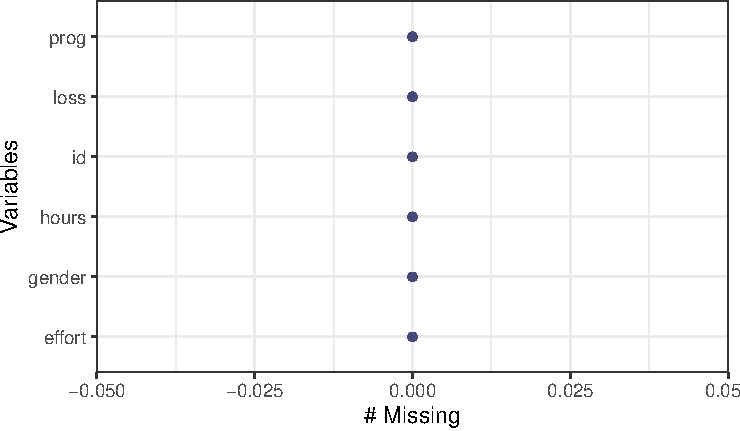
\includegraphics{Appendix_ex_weightloss_files/figure-latex/unnamed-chunk-12-1} \hfill{}

\caption{Amount of Missing Data by Variable}\label{fig:unnamed-chunk-12}
\end{figure}

\clearpage

\hypertarget{descriptive-summary}{%
\subsection{Descriptive Summary}\label{descriptive-summary}}

\begin{Shaded}
\begin{Highlighting}[]
\NormalTok{tab\_5numsum }\OtherTok{\textless{}{-}}\NormalTok{ df\_use }\SpecialCharTok{\%\textgreater{}\%} 
\NormalTok{  dplyr}\SpecialCharTok{::}\FunctionTok{select\_if}\NormalTok{(is.numeric) }\SpecialCharTok{\%\textgreater{}\%} 
\NormalTok{  psych}\SpecialCharTok{::}\FunctionTok{describe}\NormalTok{(}\AttributeTok{quant =} \FunctionTok{c}\NormalTok{(.}\DecValTok{25}\NormalTok{, .}\DecValTok{75}\NormalTok{)) }\SpecialCharTok{\%\textgreater{}\%} 
  \FunctionTok{data.frame}\NormalTok{() }\SpecialCharTok{\%\textgreater{}\%} 
\NormalTok{  dplyr}\SpecialCharTok{::}\FunctionTok{mutate}\NormalTok{(}\AttributeTok{n =} \FunctionTok{as.character}\NormalTok{(n)) }\SpecialCharTok{\%\textgreater{}\%}
\NormalTok{  tibble}\SpecialCharTok{::}\FunctionTok{rownames\_to\_column}\NormalTok{(}\AttributeTok{var =} \StringTok{"Variable"}\NormalTok{) }\SpecialCharTok{\%\textgreater{}\%} 
\NormalTok{  dplyr}\SpecialCharTok{::}\FunctionTok{mutate\_if}\NormalTok{(is.numeric, apaSupp}\SpecialCharTok{::}\NormalTok{apa2) }\SpecialCharTok{\%\textgreater{}\%} 
\NormalTok{  dplyr}\SpecialCharTok{::}\FunctionTok{select}\NormalTok{(Variable,}
                \StringTok{"n"} \OtherTok{=}\NormalTok{ n, }
                \StringTok{"Min"} \OtherTok{=}\NormalTok{ min, }
                \StringTok{"Q1"} \OtherTok{=}\NormalTok{ Q0}\FloatTok{.25}\NormalTok{, }
                \StringTok{"Mdn"} \OtherTok{=}\NormalTok{ median, }
                \StringTok{"Q3"} \OtherTok{=}\NormalTok{ Q0}\FloatTok{.75}\NormalTok{, }
                \StringTok{"Max"} \OtherTok{=}\NormalTok{ max) }\SpecialCharTok{\%\textgreater{}\%} 
\NormalTok{  flextable}\SpecialCharTok{::}\FunctionTok{flextable}\NormalTok{() }\SpecialCharTok{\%\textgreater{}\%} 
\NormalTok{  flextable}\SpecialCharTok{::}\FunctionTok{set\_caption}\NormalTok{(}\StringTok{"Five{-}Number Summary for Quantitative Measures"}\NormalTok{)}

\NormalTok{tab\_5numsum}
\end{Highlighting}
\end{Shaded}

\global\setlength{\Oldarrayrulewidth}{\arrayrulewidth}

\global\setlength{\Oldtabcolsep}{\tabcolsep}

\setlength{\tabcolsep}{2pt}

\renewcommand*{\arraystretch}{1.5}



\providecommand{\ascline}[3]{\noalign{\global\arrayrulewidth #1}\arrayrulecolor[HTML]{#2}\cline{#3}}

\begin{longtable}[l]{|p{0.75in}|p{0.75in}|p{0.75in}|p{0.75in}|p{0.75in}|p{0.75in}|p{0.75in}}

\caption{Five-Number\ Summary\ for\ Quantitative\ Measures}\\

\ascline{0.75pt}{000000}{1-7}

\multicolumn{1}{>{\centering}m{\dimexpr 0.75in+0\tabcolsep}}{\textcolor[HTML]{000000}{\fontsize{10}{20}\selectfont{\global\setmainfont{Times New Roman}{Variable}}}} & \multicolumn{1}{>{\centering}m{\dimexpr 0.75in+0\tabcolsep}}{\textcolor[HTML]{000000}{\fontsize{10}{20}\selectfont{\global\setmainfont{Times New Roman}{n}}}} & \multicolumn{1}{>{\centering}m{\dimexpr 0.75in+0\tabcolsep}}{\textcolor[HTML]{000000}{\fontsize{10}{20}\selectfont{\global\setmainfont{Times New Roman}{Min}}}} & \multicolumn{1}{>{\centering}m{\dimexpr 0.75in+0\tabcolsep}}{\textcolor[HTML]{000000}{\fontsize{10}{20}\selectfont{\global\setmainfont{Times New Roman}{Q1}}}} & \multicolumn{1}{>{\centering}m{\dimexpr 0.75in+0\tabcolsep}}{\textcolor[HTML]{000000}{\fontsize{10}{20}\selectfont{\global\setmainfont{Times New Roman}{Mdn}}}} & \multicolumn{1}{>{\centering}m{\dimexpr 0.75in+0\tabcolsep}}{\textcolor[HTML]{000000}{\fontsize{10}{20}\selectfont{\global\setmainfont{Times New Roman}{Q3}}}} & \multicolumn{1}{>{\centering}m{\dimexpr 0.75in+0\tabcolsep}}{\textcolor[HTML]{000000}{\fontsize{10}{20}\selectfont{\global\setmainfont{Times New Roman}{Max}}}} \\

\ascline{0.75pt}{000000}{1-7}\endfirsthead \caption[]{Five-Number\ Summary\ for\ Quantitative\ Measures}\\

\ascline{0.75pt}{000000}{1-7}

\multicolumn{1}{>{\centering}m{\dimexpr 0.75in+0\tabcolsep}}{\textcolor[HTML]{000000}{\fontsize{10}{20}\selectfont{\global\setmainfont{Times New Roman}{Variable}}}} & \multicolumn{1}{>{\centering}m{\dimexpr 0.75in+0\tabcolsep}}{\textcolor[HTML]{000000}{\fontsize{10}{20}\selectfont{\global\setmainfont{Times New Roman}{n}}}} & \multicolumn{1}{>{\centering}m{\dimexpr 0.75in+0\tabcolsep}}{\textcolor[HTML]{000000}{\fontsize{10}{20}\selectfont{\global\setmainfont{Times New Roman}{Min}}}} & \multicolumn{1}{>{\centering}m{\dimexpr 0.75in+0\tabcolsep}}{\textcolor[HTML]{000000}{\fontsize{10}{20}\selectfont{\global\setmainfont{Times New Roman}{Q1}}}} & \multicolumn{1}{>{\centering}m{\dimexpr 0.75in+0\tabcolsep}}{\textcolor[HTML]{000000}{\fontsize{10}{20}\selectfont{\global\setmainfont{Times New Roman}{Mdn}}}} & \multicolumn{1}{>{\centering}m{\dimexpr 0.75in+0\tabcolsep}}{\textcolor[HTML]{000000}{\fontsize{10}{20}\selectfont{\global\setmainfont{Times New Roman}{Q3}}}} & \multicolumn{1}{>{\centering}m{\dimexpr 0.75in+0\tabcolsep}}{\textcolor[HTML]{000000}{\fontsize{10}{20}\selectfont{\global\setmainfont{Times New Roman}{Max}}}} \\

\ascline{0.75pt}{000000}{1-7}\endhead



\multicolumn{1}{>{\centering}m{\dimexpr 0.75in+0\tabcolsep}}{\textcolor[HTML]{000000}{\fontsize{10}{20}\selectfont{\global\setmainfont{Times New Roman}{loss}}}} & \multicolumn{1}{>{\centering}m{\dimexpr 0.75in+0\tabcolsep}}{\textcolor[HTML]{000000}{\fontsize{10}{20}\selectfont{\global\setmainfont{Times New Roman}{900}}}} & \multicolumn{1}{>{\centering}m{\dimexpr 0.75in+0\tabcolsep}}{\textcolor[HTML]{000000}{\fontsize{10}{20}\selectfont{\global\setmainfont{Times New Roman}{-17.14}}}} & \multicolumn{1}{>{\centering}m{\dimexpr 0.75in+0\tabcolsep}}{\textcolor[HTML]{000000}{\fontsize{10}{20}\selectfont{\global\setmainfont{Times New Roman}{-1.74}}}} & \multicolumn{1}{>{\centering}m{\dimexpr 0.75in+0\tabcolsep}}{\textcolor[HTML]{000000}{\fontsize{10}{20}\selectfont{\global\setmainfont{Times New Roman}{\ 7.88}}}} & \multicolumn{1}{>{\centering}m{\dimexpr 0.75in+0\tabcolsep}}{\textcolor[HTML]{000000}{\fontsize{10}{20}\selectfont{\global\setmainfont{Times New Roman}{20.05}}}} & \multicolumn{1}{>{\centering}m{\dimexpr 0.75in+0\tabcolsep}}{\textcolor[HTML]{000000}{\fontsize{10}{20}\selectfont{\global\setmainfont{Times New Roman}{54.15}}}} \\





\multicolumn{1}{>{\centering}m{\dimexpr 0.75in+0\tabcolsep}}{\textcolor[HTML]{000000}{\fontsize{10}{20}\selectfont{\global\setmainfont{Times New Roman}{hours}}}} & \multicolumn{1}{>{\centering}m{\dimexpr 0.75in+0\tabcolsep}}{\textcolor[HTML]{000000}{\fontsize{10}{20}\selectfont{\global\setmainfont{Times New Roman}{900}}}} & \multicolumn{1}{>{\centering}m{\dimexpr 0.75in+0\tabcolsep}}{\textcolor[HTML]{000000}{\fontsize{10}{20}\selectfont{\global\setmainfont{Times New Roman}{\ \ 0.18}}}} & \multicolumn{1}{>{\centering}m{\dimexpr 0.75in+0\tabcolsep}}{\textcolor[HTML]{000000}{\fontsize{10}{20}\selectfont{\global\setmainfont{Times New Roman}{\ 1.68}}}} & \multicolumn{1}{>{\centering}m{\dimexpr 0.75in+0\tabcolsep}}{\textcolor[HTML]{000000}{\fontsize{10}{20}\selectfont{\global\setmainfont{Times New Roman}{\ 2.01}}}} & \multicolumn{1}{>{\centering}m{\dimexpr 0.75in+0\tabcolsep}}{\textcolor[HTML]{000000}{\fontsize{10}{20}\selectfont{\global\setmainfont{Times New Roman}{\ 2.34}}}} & \multicolumn{1}{>{\centering}m{\dimexpr 0.75in+0\tabcolsep}}{\textcolor[HTML]{000000}{\fontsize{10}{20}\selectfont{\global\setmainfont{Times New Roman}{\ 4.07}}}} \\





\multicolumn{1}{>{\centering}m{\dimexpr 0.75in+0\tabcolsep}}{\textcolor[HTML]{000000}{\fontsize{10}{20}\selectfont{\global\setmainfont{Times New Roman}{effort}}}} & \multicolumn{1}{>{\centering}m{\dimexpr 0.75in+0\tabcolsep}}{\textcolor[HTML]{000000}{\fontsize{10}{20}\selectfont{\global\setmainfont{Times New Roman}{900}}}} & \multicolumn{1}{>{\centering}m{\dimexpr 0.75in+0\tabcolsep}}{\textcolor[HTML]{000000}{\fontsize{10}{20}\selectfont{\global\setmainfont{Times New Roman}{\ 12.95}}}} & \multicolumn{1}{>{\centering}m{\dimexpr 0.75in+0\tabcolsep}}{\textcolor[HTML]{000000}{\fontsize{10}{20}\selectfont{\global\setmainfont{Times New Roman}{26.26}}}} & \multicolumn{1}{>{\centering}m{\dimexpr 0.75in+0\tabcolsep}}{\textcolor[HTML]{000000}{\fontsize{10}{20}\selectfont{\global\setmainfont{Times New Roman}{29.63}}}} & \multicolumn{1}{>{\centering}m{\dimexpr 0.75in+0\tabcolsep}}{\textcolor[HTML]{000000}{\fontsize{10}{20}\selectfont{\global\setmainfont{Times New Roman}{33.10}}}} & \multicolumn{1}{>{\centering}m{\dimexpr 0.75in+0\tabcolsep}}{\textcolor[HTML]{000000}{\fontsize{10}{20}\selectfont{\global\setmainfont{Times New Roman}{44.08}}}} \\

\ascline{0.75pt}{000000}{1-7}



\end{longtable}



\arrayrulecolor[HTML]{000000}

\global\setlength{\arrayrulewidth}{\Oldarrayrulewidth}

\global\setlength{\tabcolsep}{\Oldtabcolsep}

\renewcommand*{\arraystretch}{1}

\clearpage

\begin{Shaded}
\begin{Highlighting}[]
\NormalTok{df\_use }\SpecialCharTok{\%\textgreater{}\%} 
\NormalTok{  furniture}\SpecialCharTok{::}\FunctionTok{table1}\NormalTok{(}\StringTok{"Gender"} \OtherTok{=}\NormalTok{ gender,}
                    \StringTok{"Weight Loss, pounds"} \OtherTok{=}\NormalTok{ loss,}
                    \StringTok{"Program Use, hours"} \OtherTok{=}\NormalTok{ hours,}
                    \StringTok{"Program Effort, rating"} \OtherTok{=}\NormalTok{ effort,}
                    \AttributeTok{splitby =}  \SpecialCharTok{\textasciitilde{}}\NormalTok{ prog,}
                    \AttributeTok{total =} \ConstantTok{TRUE}\NormalTok{,}
                    \AttributeTok{test =} \ConstantTok{TRUE}\NormalTok{,}
                    \CommentTok{\# na.rm = FALSE,}
                    \AttributeTok{output =} \StringTok{"markdown"}\NormalTok{,}
                    \AttributeTok{digits =} \DecValTok{2}\NormalTok{,}
                    \AttributeTok{caption =} \StringTok{"Descriptive Summary of Sample, by Program"}\NormalTok{,}
                    \AttributeTok{export =} \StringTok{"tab\_descriptives"}\NormalTok{)}
\end{Highlighting}
\end{Shaded}

\begin{longtable}[]{@{}
  >{\raggedright\arraybackslash}p{(\columnwidth - 10\tabcolsep) * \real{0.2667}}
  >{\raggedright\arraybackslash}p{(\columnwidth - 10\tabcolsep) * \real{0.1667}}
  >{\raggedright\arraybackslash}p{(\columnwidth - 10\tabcolsep) * \real{0.1556}}
  >{\raggedright\arraybackslash}p{(\columnwidth - 10\tabcolsep) * \real{0.1556}}
  >{\raggedright\arraybackslash}p{(\columnwidth - 10\tabcolsep) * \real{0.1556}}
  >{\raggedright\arraybackslash}p{(\columnwidth - 10\tabcolsep) * \real{0.1000}}@{}}
\caption{Descriptive Summary of Sample, by Program}\tabularnewline
\toprule\noalign{}
\begin{minipage}[b]{\linewidth}\raggedright
\end{minipage} & \begin{minipage}[b]{\linewidth}\raggedright
Total
\end{minipage} & \begin{minipage}[b]{\linewidth}\raggedright
Jogging
\end{minipage} & \begin{minipage}[b]{\linewidth}\raggedright
Swimming
\end{minipage} & \begin{minipage}[b]{\linewidth}\raggedright
Reading
\end{minipage} & \begin{minipage}[b]{\linewidth}\raggedright
P-Value
\end{minipage} \\
\midrule\noalign{}
\endfirsthead
\toprule\noalign{}
\begin{minipage}[b]{\linewidth}\raggedright
\end{minipage} & \begin{minipage}[b]{\linewidth}\raggedright
Total
\end{minipage} & \begin{minipage}[b]{\linewidth}\raggedright
Jogging
\end{minipage} & \begin{minipage}[b]{\linewidth}\raggedright
Swimming
\end{minipage} & \begin{minipage}[b]{\linewidth}\raggedright
Reading
\end{minipage} & \begin{minipage}[b]{\linewidth}\raggedright
P-Value
\end{minipage} \\
\midrule\noalign{}
\endhead
\bottomrule\noalign{}
\endlastfoot
& n = 900 & n = 300 & n = 300 & n = 300 & \\
Gender & & & & & 1 \\
Male & 450 (50\%) & 150 (50\%) & 150 (50\%) & 150 (50\%) & \\
Female & 450 (50\%) & 150 (50\%) & 150 (50\%) & 150 (50\%) & \\
Weight Loss, pounds & & & & & \textless.001 \\
& 10.02 (14.10) & 8.03 (7.45) & 25.82 (8.92) & -3.79 (4.11) & \\
Program Use, hours & & & & & 0.469 \\
& 2.00 (0.49) & 1.99 (0.47) & 1.99 (0.48) & 2.03 (0.53) & \\
Program Effort, rating & & & & & 0.18 \\
& 29.66 (5.14) & 30.05 (5.04) & 29.65 (5.17) & 29.28 (5.20) & \\
\end{longtable}

\clearpage

\hypertarget{correlations}{%
\subsection{Correlations}\label{correlations}}

\begin{Shaded}
\begin{Highlighting}[]
\NormalTok{tab\_cor }\OtherTok{\textless{}{-}}\NormalTok{ df\_use }\SpecialCharTok{\%\textgreater{}\%} 
\NormalTok{  dplyr}\SpecialCharTok{::}\FunctionTok{select}\NormalTok{(}\StringTok{"Program Time"} \OtherTok{=}\NormalTok{ hours, }
                \StringTok{"Effort Rating"} \OtherTok{=}\NormalTok{ effort, }
                \StringTok{"Weight Loss"} \OtherTok{=}\NormalTok{ loss) }\SpecialCharTok{\%\textgreater{}\%} 
\NormalTok{  rstatix}\SpecialCharTok{::}\FunctionTok{cor\_mat}\NormalTok{() }\SpecialCharTok{\%\textgreater{}\%} 
\NormalTok{  rstatix}\SpecialCharTok{::}\FunctionTok{pull\_lower\_triangle}\NormalTok{() }\SpecialCharTok{\%\textgreater{}\%}
\NormalTok{  dplyr}\SpecialCharTok{::}\FunctionTok{rename}\NormalTok{(}\AttributeTok{Variables =}\NormalTok{ rowname) }\SpecialCharTok{\%\textgreater{}\%} 
\NormalTok{  flextable}\SpecialCharTok{::}\FunctionTok{flextable}\NormalTok{() }\SpecialCharTok{\%\textgreater{}\%} 
\NormalTok{  flextable}\SpecialCharTok{::}\FunctionTok{width}\NormalTok{(}\AttributeTok{j =} \DecValTok{1}\NormalTok{, }\AttributeTok{width =} \DecValTok{2}\NormalTok{, }\AttributeTok{unit =} \StringTok{"in"}\NormalTok{) }\SpecialCharTok{\%\textgreater{}\%} 
\NormalTok{  flextable}\SpecialCharTok{::}\FunctionTok{width}\NormalTok{(}\AttributeTok{j =} \DecValTok{2}\SpecialCharTok{:}\DecValTok{4}\NormalTok{, }\AttributeTok{width =} \DecValTok{1}\NormalTok{, }\AttributeTok{unit =} \StringTok{"in"}\NormalTok{) }\SpecialCharTok{\%\textgreater{}\%} 
\NormalTok{  flextable}\SpecialCharTok{::}\FunctionTok{colformat\_double}\NormalTok{(}\AttributeTok{digits =} \DecValTok{3}\NormalTok{) }\SpecialCharTok{\%\textgreater{}\%} 
\NormalTok{  flextable}\SpecialCharTok{::}\FunctionTok{set\_caption}\NormalTok{(}\StringTok{"Correlation Matrix for Quantitative Measures, Pearson\textquotesingle{}s Product Moment Correlation (r)"}\NormalTok{)}

\NormalTok{tab\_cor}
\end{Highlighting}
\end{Shaded}

\global\setlength{\Oldarrayrulewidth}{\arrayrulewidth}

\global\setlength{\Oldtabcolsep}{\tabcolsep}

\setlength{\tabcolsep}{2pt}

\renewcommand*{\arraystretch}{1.5}



\providecommand{\ascline}[3]{\noalign{\global\arrayrulewidth #1}\arrayrulecolor[HTML]{#2}\cline{#3}}

\begin{longtable}[l]{|p{2.00in}|p{1.00in}|p{1.00in}|p{1.00in}}

\caption{Correlation\ Matrix\ for\ Quantitative\ Measures,\ Pearson's\ Product\ Moment\ Correlation\ (r)}\\

\ascline{0.75pt}{000000}{1-4}

\multicolumn{1}{>{\centering}m{\dimexpr 2in+0\tabcolsep}}{\textcolor[HTML]{000000}{\fontsize{10}{20}\selectfont{\global\setmainfont{Times New Roman}{Variables}}}} & \multicolumn{1}{>{\centering}m{\dimexpr 1in+0\tabcolsep}}{\textcolor[HTML]{000000}{\fontsize{10}{20}\selectfont{\global\setmainfont{Times New Roman}{Program\ Time}}}} & \multicolumn{1}{>{\centering}m{\dimexpr 1in+0\tabcolsep}}{\textcolor[HTML]{000000}{\fontsize{10}{20}\selectfont{\global\setmainfont{Times New Roman}{Effort\ Rating}}}} & \multicolumn{1}{>{\centering}m{\dimexpr 1in+0\tabcolsep}}{\textcolor[HTML]{000000}{\fontsize{10}{20}\selectfont{\global\setmainfont{Times New Roman}{Weight\ Loss}}}} \\

\ascline{0.75pt}{000000}{1-4}\endfirsthead \caption[]{Correlation\ Matrix\ for\ Quantitative\ Measures,\ Pearson's\ Product\ Moment\ Correlation\ (r)}\\

\ascline{0.75pt}{000000}{1-4}

\multicolumn{1}{>{\centering}m{\dimexpr 2in+0\tabcolsep}}{\textcolor[HTML]{000000}{\fontsize{10}{20}\selectfont{\global\setmainfont{Times New Roman}{Variables}}}} & \multicolumn{1}{>{\centering}m{\dimexpr 1in+0\tabcolsep}}{\textcolor[HTML]{000000}{\fontsize{10}{20}\selectfont{\global\setmainfont{Times New Roman}{Program\ Time}}}} & \multicolumn{1}{>{\centering}m{\dimexpr 1in+0\tabcolsep}}{\textcolor[HTML]{000000}{\fontsize{10}{20}\selectfont{\global\setmainfont{Times New Roman}{Effort\ Rating}}}} & \multicolumn{1}{>{\centering}m{\dimexpr 1in+0\tabcolsep}}{\textcolor[HTML]{000000}{\fontsize{10}{20}\selectfont{\global\setmainfont{Times New Roman}{Weight\ Loss}}}} \\

\ascline{0.75pt}{000000}{1-4}\endhead



\multicolumn{1}{>{\centering}m{\dimexpr 2in+0\tabcolsep}}{\textcolor[HTML]{000000}{\fontsize{10}{20}\selectfont{\global\setmainfont{Times New Roman}{Program\ Time}}}} & \multicolumn{1}{>{\centering}m{\dimexpr 1in+0\tabcolsep}}{\textcolor[HTML]{000000}{\fontsize{10}{20}\selectfont{\global\setmainfont{Times New Roman}{}}}} & \multicolumn{1}{>{\centering}m{\dimexpr 1in+0\tabcolsep}}{\textcolor[HTML]{000000}{\fontsize{10}{20}\selectfont{\global\setmainfont{Times New Roman}{}}}} & \multicolumn{1}{>{\centering}m{\dimexpr 1in+0\tabcolsep}}{\textcolor[HTML]{000000}{\fontsize{10}{20}\selectfont{\global\setmainfont{Times New Roman}{}}}} \\





\multicolumn{1}{>{\centering}m{\dimexpr 2in+0\tabcolsep}}{\textcolor[HTML]{000000}{\fontsize{10}{20}\selectfont{\global\setmainfont{Times New Roman}{Effort\ Rating}}}} & \multicolumn{1}{>{\centering}m{\dimexpr 1in+0\tabcolsep}}{\textcolor[HTML]{000000}{\fontsize{10}{20}\selectfont{\global\setmainfont{Times New Roman}{0.016}}}} & \multicolumn{1}{>{\centering}m{\dimexpr 1in+0\tabcolsep}}{\textcolor[HTML]{000000}{\fontsize{10}{20}\selectfont{\global\setmainfont{Times New Roman}{}}}} & \multicolumn{1}{>{\centering}m{\dimexpr 1in+0\tabcolsep}}{\textcolor[HTML]{000000}{\fontsize{10}{20}\selectfont{\global\setmainfont{Times New Roman}{}}}} \\





\multicolumn{1}{>{\centering}m{\dimexpr 2in+0\tabcolsep}}{\textcolor[HTML]{000000}{\fontsize{10}{20}\selectfont{\global\setmainfont{Times New Roman}{Weight\ Loss}}}} & \multicolumn{1}{>{\centering}m{\dimexpr 1in+0\tabcolsep}}{\textcolor[HTML]{000000}{\fontsize{10}{20}\selectfont{\global\setmainfont{Times New Roman}{0.087}}}} & \multicolumn{1}{>{\centering}m{\dimexpr 1in+0\tabcolsep}}{\textcolor[HTML]{000000}{\fontsize{10}{20}\selectfont{\global\setmainfont{Times New Roman}{0.26}}}} & \multicolumn{1}{>{\centering}m{\dimexpr 1in+0\tabcolsep}}{\textcolor[HTML]{000000}{\fontsize{10}{20}\selectfont{\global\setmainfont{Times New Roman}{}}}} \\

\ascline{0.75pt}{000000}{1-4}



\end{longtable}



\arrayrulecolor[HTML]{000000}

\global\setlength{\arrayrulewidth}{\Oldarrayrulewidth}

\global\setlength{\tabcolsep}{\Oldtabcolsep}

\renewcommand*{\arraystretch}{1}

\clearpage

\begin{Shaded}
\begin{Highlighting}[]
\NormalTok{tab\_cor\_gather }\OtherTok{\textless{}{-}}\NormalTok{ df\_use }\SpecialCharTok{\%\textgreater{}\%} 
\NormalTok{  dplyr}\SpecialCharTok{::}\FunctionTok{select}\NormalTok{(}\StringTok{"Hours"} \OtherTok{=}\NormalTok{ hours, }
                \StringTok{"Effort"} \OtherTok{=}\NormalTok{ effort, }
                \StringTok{"Loss"} \OtherTok{=}\NormalTok{ loss) }\SpecialCharTok{\%\textgreater{}\%} 
\NormalTok{  rstatix}\SpecialCharTok{::}\FunctionTok{cor\_mat}\NormalTok{() }\SpecialCharTok{\%\textgreater{}\%} 
\NormalTok{  rstatix}\SpecialCharTok{::}\FunctionTok{cor\_gather}\NormalTok{() }\SpecialCharTok{\%\textgreater{}\%} 
\NormalTok{  dplyr}\SpecialCharTok{::}\FunctionTok{mutate}\NormalTok{(}\AttributeTok{p =}\NormalTok{ apaSupp}\SpecialCharTok{::}\FunctionTok{p\_num}\NormalTok{(p)) }\SpecialCharTok{\%\textgreater{}\%} 
\NormalTok{  dplyr}\SpecialCharTok{::}\FunctionTok{filter}\NormalTok{(cor }\SpecialCharTok{\textless{}} \DecValTok{1}\NormalTok{) }\SpecialCharTok{\%\textgreater{}\%} 
\NormalTok{  dplyr}\SpecialCharTok{::}\FunctionTok{group\_by}\NormalTok{(cor, p) }\SpecialCharTok{\%\textgreater{}\%} 
\NormalTok{  dplyr}\SpecialCharTok{::}\FunctionTok{slice}\NormalTok{(}\DecValTok{1}\NormalTok{) }\SpecialCharTok{\%\textgreater{}\%} 
\NormalTok{  dplyr}\SpecialCharTok{::}\FunctionTok{ungroup}\NormalTok{() }\SpecialCharTok{\%\textgreater{}\%} 
\NormalTok{  tidyr}\SpecialCharTok{::}\FunctionTok{unite}\NormalTok{(}\AttributeTok{col =} \StringTok{"Variables"}\NormalTok{, var1, var2, }\AttributeTok{sep =} \StringTok{" \& "}\NormalTok{) }\SpecialCharTok{\%\textgreater{}\%} 
\NormalTok{  dplyr}\SpecialCharTok{::}\FunctionTok{rename}\NormalTok{(}\StringTok{"r"} \OtherTok{=} \StringTok{"cor"}\NormalTok{) }\SpecialCharTok{\%\textgreater{}\%} 
\NormalTok{  flextable}\SpecialCharTok{::}\FunctionTok{flextable}\NormalTok{() }\SpecialCharTok{\%\textgreater{}\%} 
\NormalTok{  flextable}\SpecialCharTok{::}\FunctionTok{width}\NormalTok{(}\AttributeTok{j =} \DecValTok{1}\NormalTok{, }\AttributeTok{width =} \DecValTok{2}\NormalTok{, }\AttributeTok{unit =} \StringTok{"in"}\NormalTok{) }\SpecialCharTok{\%\textgreater{}\%} 
\NormalTok{  flextable}\SpecialCharTok{::}\FunctionTok{width}\NormalTok{(}\AttributeTok{j =} \DecValTok{2}\SpecialCharTok{:}\DecValTok{3}\NormalTok{, }\AttributeTok{width =} \FloatTok{1.5}\NormalTok{, }\AttributeTok{unit =} \StringTok{"in"}\NormalTok{) }\SpecialCharTok{\%\textgreater{}\%} 
\NormalTok{  flextable}\SpecialCharTok{::}\FunctionTok{colformat\_double}\NormalTok{(}\AttributeTok{digits =} \DecValTok{3}\NormalTok{) }\SpecialCharTok{\%\textgreater{}\%} 
\NormalTok{  flextable}\SpecialCharTok{::}\FunctionTok{set\_caption}\NormalTok{(}\StringTok{"Correlations for Quantitative Measurse, Pearson\textquotesingle{}s Product Moment Correlation (r) and Statistical Significance (p)"}\NormalTok{)}

\NormalTok{tab\_cor\_gather}
\end{Highlighting}
\end{Shaded}

\global\setlength{\Oldarrayrulewidth}{\arrayrulewidth}

\global\setlength{\Oldtabcolsep}{\tabcolsep}

\setlength{\tabcolsep}{2pt}

\renewcommand*{\arraystretch}{1.5}



\providecommand{\ascline}[3]{\noalign{\global\arrayrulewidth #1}\arrayrulecolor[HTML]{#2}\cline{#3}}

\begin{longtable}[l]{|p{2.00in}|p{1.50in}|p{1.50in}}

\caption{Correlations\ for\ Quantitative\ Measurse,\ Pearson's\ Product\ Moment\ Correlation\ (r)\ and\ Statistical\ Significance\ (p)}\\

\ascline{0.75pt}{000000}{1-3}

\multicolumn{1}{>{\centering}m{\dimexpr 2in+0\tabcolsep}}{\textcolor[HTML]{000000}{\fontsize{10}{20}\selectfont{\global\setmainfont{Times New Roman}{Variables}}}} & \multicolumn{1}{>{\centering}m{\dimexpr 1.5in+0\tabcolsep}}{\textcolor[HTML]{000000}{\fontsize{10}{20}\selectfont{\global\setmainfont{Times New Roman}{r}}}} & \multicolumn{1}{>{\centering}m{\dimexpr 1.5in+0\tabcolsep}}{\textcolor[HTML]{000000}{\fontsize{10}{20}\selectfont{\global\setmainfont{Times New Roman}{p}}}} \\

\ascline{0.75pt}{000000}{1-3}\endfirsthead \caption[]{Correlations\ for\ Quantitative\ Measurse,\ Pearson's\ Product\ Moment\ Correlation\ (r)\ and\ Statistical\ Significance\ (p)}\\

\ascline{0.75pt}{000000}{1-3}

\multicolumn{1}{>{\centering}m{\dimexpr 2in+0\tabcolsep}}{\textcolor[HTML]{000000}{\fontsize{10}{20}\selectfont{\global\setmainfont{Times New Roman}{Variables}}}} & \multicolumn{1}{>{\centering}m{\dimexpr 1.5in+0\tabcolsep}}{\textcolor[HTML]{000000}{\fontsize{10}{20}\selectfont{\global\setmainfont{Times New Roman}{r}}}} & \multicolumn{1}{>{\centering}m{\dimexpr 1.5in+0\tabcolsep}}{\textcolor[HTML]{000000}{\fontsize{10}{20}\selectfont{\global\setmainfont{Times New Roman}{p}}}} \\

\ascline{0.75pt}{000000}{1-3}\endhead



\multicolumn{1}{>{\centering}m{\dimexpr 2in+0\tabcolsep}}{\textcolor[HTML]{000000}{\fontsize{10}{20}\selectfont{\global\setmainfont{Times New Roman}{Effort\ \&\ Hours}}}} & \multicolumn{1}{>{\centering}m{\dimexpr 1.5in+0\tabcolsep}}{\textcolor[HTML]{000000}{\fontsize{10}{20}\selectfont{\global\setmainfont{Times New Roman}{0.016}}}} & \multicolumn{1}{>{\centering}m{\dimexpr 1.5in+0\tabcolsep}}{\textcolor[HTML]{000000}{\fontsize{10}{20}\selectfont{\global\setmainfont{Times New Roman}{.626}}}} \\





\multicolumn{1}{>{\centering}m{\dimexpr 2in+0\tabcolsep}}{\textcolor[HTML]{000000}{\fontsize{10}{20}\selectfont{\global\setmainfont{Times New Roman}{Loss\ \&\ Hours}}}} & \multicolumn{1}{>{\centering}m{\dimexpr 1.5in+0\tabcolsep}}{\textcolor[HTML]{000000}{\fontsize{10}{20}\selectfont{\global\setmainfont{Times New Roman}{0.087}}}} & \multicolumn{1}{>{\centering}m{\dimexpr 1.5in+0\tabcolsep}}{\textcolor[HTML]{000000}{\fontsize{10}{20}\selectfont{\global\setmainfont{Times New Roman}{.009\ **}}}} \\





\multicolumn{1}{>{\centering}m{\dimexpr 2in+0\tabcolsep}}{\textcolor[HTML]{000000}{\fontsize{10}{20}\selectfont{\global\setmainfont{Times New Roman}{Loss\ \&\ Effort}}}} & \multicolumn{1}{>{\centering}m{\dimexpr 1.5in+0\tabcolsep}}{\textcolor[HTML]{000000}{\fontsize{10}{20}\selectfont{\global\setmainfont{Times New Roman}{0.260}}}} & \multicolumn{1}{>{\centering}m{\dimexpr 1.5in+0\tabcolsep}}{\textcolor[HTML]{000000}{\fontsize{10}{20}\selectfont{\global\setmainfont{Times New Roman}{<\ .001\ ***}}}} \\

\ascline{0.75pt}{000000}{1-3}



\end{longtable}



\arrayrulecolor[HTML]{000000}

\global\setlength{\arrayrulewidth}{\Oldarrayrulewidth}

\global\setlength{\tabcolsep}{\Oldtabcolsep}

\renewcommand*{\arraystretch}{1}

\clearpage

\begin{Shaded}
\begin{Highlighting}[]
\NormalTok{tab\_cor\_split }\OtherTok{\textless{}{-}}\NormalTok{ df\_use }\SpecialCharTok{\%\textgreater{}\%} 
\NormalTok{  dplyr}\SpecialCharTok{::}\FunctionTok{group\_by}\NormalTok{(prog, gender) }\SpecialCharTok{\%\textgreater{}\%} 
\NormalTok{  dplyr}\SpecialCharTok{::}\FunctionTok{select}\NormalTok{(}\StringTok{"Hours"} \OtherTok{=}\NormalTok{ hours, }
                \StringTok{"Effort"} \OtherTok{=}\NormalTok{ effort, }
                \StringTok{"Loss"} \OtherTok{=}\NormalTok{ loss) }\SpecialCharTok{\%\textgreater{}\%} 
\NormalTok{  tidyr}\SpecialCharTok{::}\FunctionTok{nest}\NormalTok{() }\SpecialCharTok{\%\textgreater{}\%} 
\NormalTok{  dplyr}\SpecialCharTok{::}\FunctionTok{mutate}\NormalTok{(}\AttributeTok{cor =} \FunctionTok{map}\NormalTok{(data, }
                          \SpecialCharTok{\textasciitilde{}}\NormalTok{ rstatix}\SpecialCharTok{::}\FunctionTok{cor\_mat}\NormalTok{(.x) }\SpecialCharTok{\%\textgreater{}\%} 
\NormalTok{                            rstatix}\SpecialCharTok{::}\FunctionTok{cor\_gather}\NormalTok{())) }\SpecialCharTok{\%\textgreater{}\%} 
\NormalTok{  tidyr}\SpecialCharTok{::}\FunctionTok{unnest}\NormalTok{(cor) }\SpecialCharTok{\%\textgreater{}\%} 
\NormalTok{  dplyr}\SpecialCharTok{::}\FunctionTok{select}\NormalTok{(}\SpecialCharTok{{-}}\NormalTok{data) }\SpecialCharTok{\%\textgreater{}\%} 
\NormalTok{  dplyr}\SpecialCharTok{::}\FunctionTok{mutate}\NormalTok{(}\AttributeTok{p =}\NormalTok{ apaSupp}\SpecialCharTok{::}\FunctionTok{p\_num}\NormalTok{(p)) }\SpecialCharTok{\%\textgreater{}\%} 
\NormalTok{  dplyr}\SpecialCharTok{::}\FunctionTok{filter}\NormalTok{(cor }\SpecialCharTok{\textless{}} \DecValTok{1}\NormalTok{) }\SpecialCharTok{\%\textgreater{}\%} 
\NormalTok{  dplyr}\SpecialCharTok{::}\FunctionTok{group\_by}\NormalTok{(prog, gender, cor, p) }\SpecialCharTok{\%\textgreater{}\%} 
\NormalTok{  dplyr}\SpecialCharTok{::}\FunctionTok{slice}\NormalTok{(}\DecValTok{1}\NormalTok{) }\SpecialCharTok{\%\textgreater{}\%} 
\NormalTok{  dplyr}\SpecialCharTok{::}\FunctionTok{ungroup}\NormalTok{() }\SpecialCharTok{\%\textgreater{}\%} 
\NormalTok{  tidyr}\SpecialCharTok{::}\FunctionTok{unite}\NormalTok{(}\AttributeTok{col =} \StringTok{"Variables"}\NormalTok{, var1, var2, }\AttributeTok{sep =} \StringTok{" \& "}\NormalTok{) }\SpecialCharTok{\%\textgreater{}\%} 
\NormalTok{  dplyr}\SpecialCharTok{::}\FunctionTok{mutate}\NormalTok{(}\AttributeTok{text =}\NormalTok{ glue}\SpecialCharTok{::}\FunctionTok{glue}\NormalTok{(}\StringTok{"\{apaSupp::apa3(cor)\} (\{p\})"}\NormalTok{)) }\SpecialCharTok{\%\textgreater{}\%} 
\NormalTok{  dplyr}\SpecialCharTok{::}\FunctionTok{select}\NormalTok{(}\SpecialCharTok{{-}}\NormalTok{cor, }\SpecialCharTok{{-}}\NormalTok{p) }\SpecialCharTok{\%\textgreater{}\%} 
\NormalTok{  tidyr}\SpecialCharTok{::}\FunctionTok{pivot\_wider}\NormalTok{(}\AttributeTok{names\_from =}\NormalTok{ Variables,}
                     \AttributeTok{values\_from =}\NormalTok{ text) }\SpecialCharTok{\%\textgreater{}\%} 
\NormalTok{  flextable}\SpecialCharTok{::}\FunctionTok{flextable}\NormalTok{() }\SpecialCharTok{\%\textgreater{}\%} 
\NormalTok{  flextable}\SpecialCharTok{::}\FunctionTok{width}\NormalTok{(}\AttributeTok{j =} \DecValTok{3}\SpecialCharTok{:}\DecValTok{5}\NormalTok{, }\AttributeTok{width =} \FloatTok{1.3}\NormalTok{, }\AttributeTok{unit =} \StringTok{"in"}\NormalTok{) }\SpecialCharTok{\%\textgreater{}\%}
\NormalTok{  flextable}\SpecialCharTok{::}\FunctionTok{set\_caption}\NormalTok{(}\StringTok{"Correlations for Quantitative Measurse, Pearson\textquotesingle{}s Product Moment Correlation, by Program and Gender"}\NormalTok{)}

\NormalTok{tab\_cor\_split}
\end{Highlighting}
\end{Shaded}

\global\setlength{\Oldarrayrulewidth}{\arrayrulewidth}

\global\setlength{\Oldtabcolsep}{\tabcolsep}

\setlength{\tabcolsep}{2pt}

\renewcommand*{\arraystretch}{1.5}



\providecommand{\ascline}[3]{\noalign{\global\arrayrulewidth #1}\arrayrulecolor[HTML]{#2}\cline{#3}}

\begin{longtable}[l]{|p{0.75in}|p{0.75in}|p{1.30in}|p{1.30in}|p{1.30in}}

\caption{Correlations\ for\ Quantitative\ Measurse,\ Pearson's\ Product\ Moment\ Correlation,\ by\ Program\ and\ Gender}\\

\ascline{0.75pt}{000000}{1-5}

\multicolumn{1}{>{\centering}m{\dimexpr 0.75in+0\tabcolsep}}{\textcolor[HTML]{000000}{\fontsize{10}{20}\selectfont{\global\setmainfont{Times New Roman}{prog}}}} & \multicolumn{1}{>{\centering}m{\dimexpr 0.75in+0\tabcolsep}}{\textcolor[HTML]{000000}{\fontsize{10}{20}\selectfont{\global\setmainfont{Times New Roman}{gender}}}} & \multicolumn{1}{>{\centering}m{\dimexpr 1.3in+0\tabcolsep}}{\textcolor[HTML]{000000}{\fontsize{10}{20}\selectfont{\global\setmainfont{Times New Roman}{Effort\ \&\ Hours}}}} & \multicolumn{1}{>{\centering}m{\dimexpr 1.3in+0\tabcolsep}}{\textcolor[HTML]{000000}{\fontsize{10}{20}\selectfont{\global\setmainfont{Times New Roman}{Loss\ \&\ Hours}}}} & \multicolumn{1}{>{\centering}m{\dimexpr 1.3in+0\tabcolsep}}{\textcolor[HTML]{000000}{\fontsize{10}{20}\selectfont{\global\setmainfont{Times New Roman}{Loss\ \&\ Effort}}}} \\

\ascline{0.75pt}{000000}{1-5}\endfirsthead \caption[]{Correlations\ for\ Quantitative\ Measurse,\ Pearson's\ Product\ Moment\ Correlation,\ by\ Program\ and\ Gender}\\

\ascline{0.75pt}{000000}{1-5}

\multicolumn{1}{>{\centering}m{\dimexpr 0.75in+0\tabcolsep}}{\textcolor[HTML]{000000}{\fontsize{10}{20}\selectfont{\global\setmainfont{Times New Roman}{prog}}}} & \multicolumn{1}{>{\centering}m{\dimexpr 0.75in+0\tabcolsep}}{\textcolor[HTML]{000000}{\fontsize{10}{20}\selectfont{\global\setmainfont{Times New Roman}{gender}}}} & \multicolumn{1}{>{\centering}m{\dimexpr 1.3in+0\tabcolsep}}{\textcolor[HTML]{000000}{\fontsize{10}{20}\selectfont{\global\setmainfont{Times New Roman}{Effort\ \&\ Hours}}}} & \multicolumn{1}{>{\centering}m{\dimexpr 1.3in+0\tabcolsep}}{\textcolor[HTML]{000000}{\fontsize{10}{20}\selectfont{\global\setmainfont{Times New Roman}{Loss\ \&\ Hours}}}} & \multicolumn{1}{>{\centering}m{\dimexpr 1.3in+0\tabcolsep}}{\textcolor[HTML]{000000}{\fontsize{10}{20}\selectfont{\global\setmainfont{Times New Roman}{Loss\ \&\ Effort}}}} \\

\ascline{0.75pt}{000000}{1-5}\endhead



\multicolumn{1}{>{\centering}m{\dimexpr 0.75in+0\tabcolsep}}{\textcolor[HTML]{000000}{\fontsize{10}{20}\selectfont{\global\setmainfont{Times New Roman}{Jogging}}}} & \multicolumn{1}{>{\centering}m{\dimexpr 0.75in+0\tabcolsep}}{\textcolor[HTML]{000000}{\fontsize{10}{20}\selectfont{\global\setmainfont{Times New Roman}{Male}}}} & \multicolumn{1}{>{\centering}m{\dimexpr 1.3in+0\tabcolsep}}{\textcolor[HTML]{000000}{\fontsize{10}{20}\selectfont{\global\setmainfont{Times New Roman}{\ 0.180\ (.030\ *)}}}} & \multicolumn{1}{>{\centering}m{\dimexpr 1.3in+0\tabcolsep}}{\textcolor[HTML]{000000}{\fontsize{10}{20}\selectfont{\global\setmainfont{Times New Roman}{\ 0.350\ (<\ .001\ ***)}}}} & \multicolumn{1}{>{\centering}m{\dimexpr 1.3in+0\tabcolsep}}{\textcolor[HTML]{000000}{\fontsize{10}{20}\selectfont{\global\setmainfont{Times New Roman}{\ 0.740\ (<\ .001\ ***)}}}} \\





\multicolumn{1}{>{\centering}m{\dimexpr 0.75in+0\tabcolsep}}{\textcolor[HTML]{000000}{\fontsize{10}{20}\selectfont{\global\setmainfont{Times New Roman}{Jogging}}}} & \multicolumn{1}{>{\centering}m{\dimexpr 0.75in+0\tabcolsep}}{\textcolor[HTML]{000000}{\fontsize{10}{20}\selectfont{\global\setmainfont{Times New Roman}{Female}}}} & \multicolumn{1}{>{\centering}m{\dimexpr 1.3in+0\tabcolsep}}{\textcolor[HTML]{000000}{\fontsize{10}{20}\selectfont{\global\setmainfont{Times New Roman}{-0.041\ (.616)}}}} & \multicolumn{1}{>{\centering}m{\dimexpr 1.3in+0\tabcolsep}}{\textcolor[HTML]{000000}{\fontsize{10}{20}\selectfont{\global\setmainfont{Times New Roman}{\ 0.650\ (<\ .001\ ***)}}}} & \multicolumn{1}{>{\centering}m{\dimexpr 1.3in+0\tabcolsep}}{\textcolor[HTML]{000000}{\fontsize{10}{20}\selectfont{\global\setmainfont{Times New Roman}{\ 0.440\ (<\ .001\ ***)}}}} \\





\multicolumn{1}{>{\centering}m{\dimexpr 0.75in+0\tabcolsep}}{\textcolor[HTML]{000000}{\fontsize{10}{20}\selectfont{\global\setmainfont{Times New Roman}{Swimming}}}} & \multicolumn{1}{>{\centering}m{\dimexpr 0.75in+0\tabcolsep}}{\textcolor[HTML]{000000}{\fontsize{10}{20}\selectfont{\global\setmainfont{Times New Roman}{Male}}}} & \multicolumn{1}{>{\centering}m{\dimexpr 1.3in+0\tabcolsep}}{\textcolor[HTML]{000000}{\fontsize{10}{20}\selectfont{\global\setmainfont{Times New Roman}{-0.049\ (.550)}}}} & \multicolumn{1}{>{\centering}m{\dimexpr 1.3in+0\tabcolsep}}{\textcolor[HTML]{000000}{\fontsize{10}{20}\selectfont{\global\setmainfont{Times New Roman}{\ 0.510\ (<\ .001\ ***)}}}} & \multicolumn{1}{>{\centering}m{\dimexpr 1.3in+0\tabcolsep}}{\textcolor[HTML]{000000}{\fontsize{10}{20}\selectfont{\global\setmainfont{Times New Roman}{\ 0.700\ (<\ .001\ ***)}}}} \\





\multicolumn{1}{>{\centering}m{\dimexpr 0.75in+0\tabcolsep}}{\textcolor[HTML]{000000}{\fontsize{10}{20}\selectfont{\global\setmainfont{Times New Roman}{Swimming}}}} & \multicolumn{1}{>{\centering}m{\dimexpr 0.75in+0\tabcolsep}}{\textcolor[HTML]{000000}{\fontsize{10}{20}\selectfont{\global\setmainfont{Times New Roman}{Female}}}} & \multicolumn{1}{>{\centering}m{\dimexpr 1.3in+0\tabcolsep}}{\textcolor[HTML]{000000}{\fontsize{10}{20}\selectfont{\global\setmainfont{Times New Roman}{-0.059\ (.473)}}}} & \multicolumn{1}{>{\centering}m{\dimexpr 1.3in+0\tabcolsep}}{\textcolor[HTML]{000000}{\fontsize{10}{20}\selectfont{\global\setmainfont{Times New Roman}{\ 0.260\ (.001\ **)}}}} & \multicolumn{1}{>{\centering}m{\dimexpr 1.3in+0\tabcolsep}}{\textcolor[HTML]{000000}{\fontsize{10}{20}\selectfont{\global\setmainfont{Times New Roman}{\ 0.780\ (<\ .001\ ***)}}}} \\





\multicolumn{1}{>{\centering}m{\dimexpr 0.75in+0\tabcolsep}}{\textcolor[HTML]{000000}{\fontsize{10}{20}\selectfont{\global\setmainfont{Times New Roman}{Reading}}}} & \multicolumn{1}{>{\centering}m{\dimexpr 0.75in+0\tabcolsep}}{\textcolor[HTML]{000000}{\fontsize{10}{20}\selectfont{\global\setmainfont{Times New Roman}{Male}}}} & \multicolumn{1}{>{\centering}m{\dimexpr 1.3in+0\tabcolsep}}{\textcolor[HTML]{000000}{\fontsize{10}{20}\selectfont{\global\setmainfont{Times New Roman}{\ 0.036\ (.661)}}}} & \multicolumn{1}{>{\centering}m{\dimexpr 1.3in+0\tabcolsep}}{\textcolor[HTML]{000000}{\fontsize{10}{20}\selectfont{\global\setmainfont{Times New Roman}{-0.470\ (<\ .001\ ***)}}}} & \multicolumn{1}{>{\centering}m{\dimexpr 1.3in+0\tabcolsep}}{\textcolor[HTML]{000000}{\fontsize{10}{20}\selectfont{\global\setmainfont{Times New Roman}{\ 0.093\ (.258)}}}} \\





\multicolumn{1}{>{\centering}m{\dimexpr 0.75in+0\tabcolsep}}{\textcolor[HTML]{000000}{\fontsize{10}{20}\selectfont{\global\setmainfont{Times New Roman}{Reading}}}} & \multicolumn{1}{>{\centering}m{\dimexpr 0.75in+0\tabcolsep}}{\textcolor[HTML]{000000}{\fontsize{10}{20}\selectfont{\global\setmainfont{Times New Roman}{Female}}}} & \multicolumn{1}{>{\centering}m{\dimexpr 1.3in+0\tabcolsep}}{\textcolor[HTML]{000000}{\fontsize{10}{20}\selectfont{\global\setmainfont{Times New Roman}{\ 0.037\ (.649)}}}} & \multicolumn{1}{>{\centering}m{\dimexpr 1.3in+0\tabcolsep}}{\textcolor[HTML]{000000}{\fontsize{10}{20}\selectfont{\global\setmainfont{Times New Roman}{-0.300\ (<\ .001\ ***)}}}} & \multicolumn{1}{>{\centering}m{\dimexpr 1.3in+0\tabcolsep}}{\textcolor[HTML]{000000}{\fontsize{10}{20}\selectfont{\global\setmainfont{Times New Roman}{\ 0.037\ (.654)}}}} \\

\ascline{0.75pt}{000000}{1-5}



\end{longtable}



\arrayrulecolor[HTML]{000000}

\global\setlength{\arrayrulewidth}{\Oldarrayrulewidth}

\global\setlength{\tabcolsep}{\Oldtabcolsep}

\renewcommand*{\arraystretch}{1}

\clearpage

\begin{Shaded}
\begin{Highlighting}[]
\NormalTok{df\_use }\SpecialCharTok{\%\textgreater{}\%} 
\NormalTok{  dplyr}\SpecialCharTok{::}\FunctionTok{select}\NormalTok{(}\StringTok{"Hours"} \OtherTok{=}\NormalTok{ hours, }
                \StringTok{"Effort"} \OtherTok{=}\NormalTok{ effort, }
                \StringTok{"Loss"} \OtherTok{=}\NormalTok{ loss) }\SpecialCharTok{\%\textgreater{}\%} 
  \FunctionTok{cor}\NormalTok{() }\SpecialCharTok{\%\textgreater{}\%} 
\NormalTok{  corrplot}\SpecialCharTok{::}\FunctionTok{corrplot.mixed}\NormalTok{()}
\end{Highlighting}
\end{Shaded}

\begin{figure}[hb]

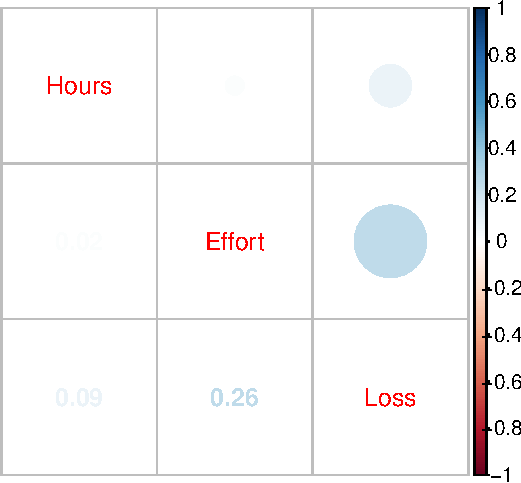
\includegraphics{Appendix_ex_weightloss_files/figure-latex/unnamed-chunk-22-1} \hfill{}

\caption{Correlation Plot for Program Time, Effort Rating, and Weight Loss, Pearson's Product Moment Correlation (r) Indication Statistical Significance - Option A}\label{fig:unnamed-chunk-22}
\end{figure}

\clearpage

\begin{Shaded}
\begin{Highlighting}[]
\NormalTok{df\_use }\SpecialCharTok{\%\textgreater{}\%} 
\NormalTok{  dplyr}\SpecialCharTok{::}\FunctionTok{select}\NormalTok{(}\StringTok{"Hours"} \OtherTok{=}\NormalTok{ hours, }
                \StringTok{"Effort"} \OtherTok{=}\NormalTok{ effort, }
                \StringTok{"Loss"} \OtherTok{=}\NormalTok{ loss) }\SpecialCharTok{\%\textgreater{}\%} 
\NormalTok{  rstatix}\SpecialCharTok{::}\FunctionTok{cor\_mat}\NormalTok{() }\SpecialCharTok{\%\textgreater{}\%}   
\NormalTok{  rstatix}\SpecialCharTok{::}\FunctionTok{cor\_reorder}\NormalTok{() }\SpecialCharTok{\%\textgreater{}\%}
\NormalTok{  rstatix}\SpecialCharTok{::}\FunctionTok{pull\_lower\_triangle}\NormalTok{() }\SpecialCharTok{\%\textgreater{}\%}
\NormalTok{  rstatix}\SpecialCharTok{::}\FunctionTok{cor\_plot}\NormalTok{(}\AttributeTok{label =} \ConstantTok{TRUE}\NormalTok{)}
\end{Highlighting}
\end{Shaded}

\begin{figure}[hb]

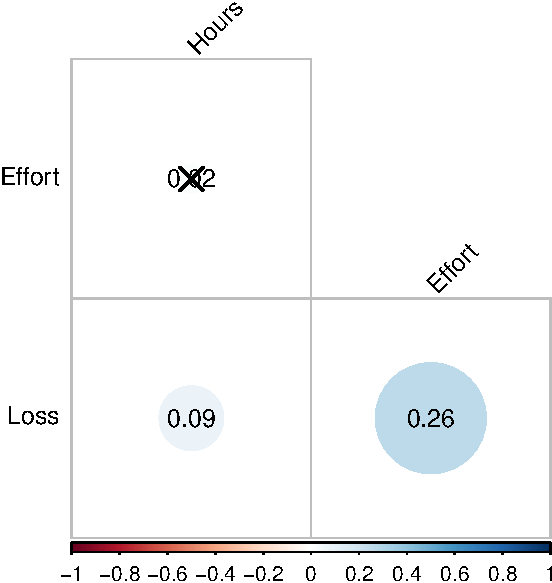
\includegraphics{Appendix_ex_weightloss_files/figure-latex/unnamed-chunk-23-1} \hfill{}

\caption{Correlation Plot for Program Time, Effort Rating, and Weight Loss, Pearson's Product Moment Correlation (r) Indication Statistical Significance - Option B}\label{fig:unnamed-chunk-23}
\end{figure}

\clearpage

\begin{Shaded}
\begin{Highlighting}[]
\NormalTok{df\_use }\SpecialCharTok{\%\textgreater{}\%} 
\NormalTok{  dplyr}\SpecialCharTok{::}\FunctionTok{filter}\NormalTok{(prog }\SpecialCharTok{==} \StringTok{"Jogging"}\NormalTok{) }\SpecialCharTok{\%\textgreater{}\%} 
\NormalTok{  dplyr}\SpecialCharTok{::}\FunctionTok{select}\NormalTok{(}\StringTok{"Hours"} \OtherTok{=}\NormalTok{ hours, }
                \StringTok{"Effort"} \OtherTok{=}\NormalTok{ effort, }
                \StringTok{"Loss"} \OtherTok{=}\NormalTok{ loss) }\SpecialCharTok{\%\textgreater{}\%} 
\NormalTok{  rstatix}\SpecialCharTok{::}\FunctionTok{cor\_mat}\NormalTok{() }\SpecialCharTok{\%\textgreater{}\%}   
\NormalTok{  rstatix}\SpecialCharTok{::}\FunctionTok{cor\_reorder}\NormalTok{() }\SpecialCharTok{\%\textgreater{}\%}
\NormalTok{  rstatix}\SpecialCharTok{::}\FunctionTok{pull\_lower\_triangle}\NormalTok{() }\SpecialCharTok{\%\textgreater{}\%}
\NormalTok{  rstatix}\SpecialCharTok{::}\FunctionTok{cor\_plot}\NormalTok{(}\AttributeTok{label =} \ConstantTok{TRUE}\NormalTok{)}
\end{Highlighting}
\end{Shaded}

\begin{figure}[hb]

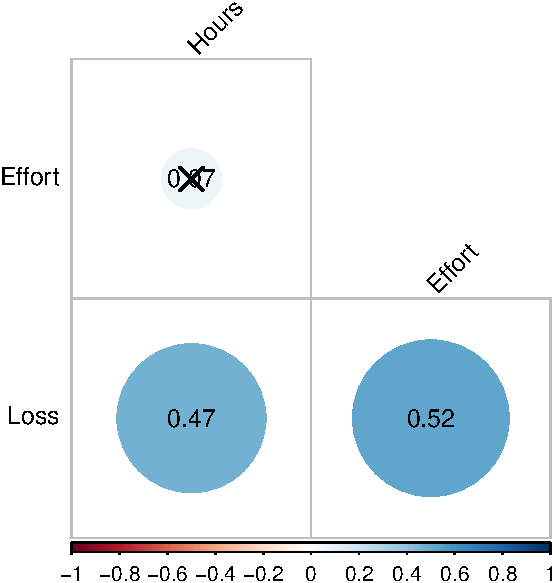
\includegraphics{Appendix_ex_weightloss_files/figure-latex/unnamed-chunk-24-1} \hfill{}

\caption{Correlation Plot for Program Time, Effort Rating, and Weight Loss, Pearson's Product Moment Correlation (r) Indication Statistical Significance, for the Jogging Program}\label{fig:unnamed-chunk-24}
\end{figure}

\clearpage

\begin{Shaded}
\begin{Highlighting}[]
\NormalTok{df\_use }\SpecialCharTok{\%\textgreater{}\%} 
\NormalTok{  dplyr}\SpecialCharTok{::}\FunctionTok{filter}\NormalTok{(prog }\SpecialCharTok{==} \StringTok{"Swimming"}\NormalTok{) }\SpecialCharTok{\%\textgreater{}\%} 
\NormalTok{  dplyr}\SpecialCharTok{::}\FunctionTok{select}\NormalTok{(}\StringTok{"Hours"} \OtherTok{=}\NormalTok{ hours, }
                \StringTok{"Effort"} \OtherTok{=}\NormalTok{ effort, }
                \StringTok{"Loss"} \OtherTok{=}\NormalTok{ loss) }\SpecialCharTok{\%\textgreater{}\%} 
\NormalTok{  rstatix}\SpecialCharTok{::}\FunctionTok{cor\_mat}\NormalTok{() }\SpecialCharTok{\%\textgreater{}\%}   
\NormalTok{  rstatix}\SpecialCharTok{::}\FunctionTok{cor\_reorder}\NormalTok{() }\SpecialCharTok{\%\textgreater{}\%}
\NormalTok{  rstatix}\SpecialCharTok{::}\FunctionTok{pull\_lower\_triangle}\NormalTok{() }\SpecialCharTok{\%\textgreater{}\%}
\NormalTok{  rstatix}\SpecialCharTok{::}\FunctionTok{cor\_plot}\NormalTok{(}\AttributeTok{label =} \ConstantTok{TRUE}\NormalTok{)}
\end{Highlighting}
\end{Shaded}

\begin{figure}[hb]

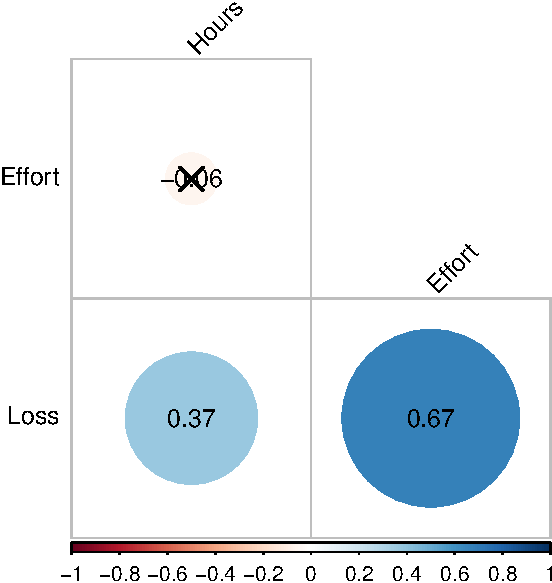
\includegraphics{Appendix_ex_weightloss_files/figure-latex/unnamed-chunk-25-1} \hfill{}

\caption{Correlation Plot for Program Time, Effort Rating, and Weight Loss, Pearson's Product Moment Correlation (r) Indication Statistical Significance, for the Swimming Running}\label{fig:unnamed-chunk-25}
\end{figure}

\clearpage

\begin{Shaded}
\begin{Highlighting}[]
\NormalTok{df\_use }\SpecialCharTok{\%\textgreater{}\%} 
\NormalTok{  dplyr}\SpecialCharTok{::}\FunctionTok{filter}\NormalTok{(prog }\SpecialCharTok{==} \StringTok{"Reading"}\NormalTok{) }\SpecialCharTok{\%\textgreater{}\%} 
\NormalTok{  dplyr}\SpecialCharTok{::}\FunctionTok{select}\NormalTok{(}\StringTok{"Hours"} \OtherTok{=}\NormalTok{ hours, }
                \StringTok{"Effort"} \OtherTok{=}\NormalTok{ effort, }
                \StringTok{"Loss"} \OtherTok{=}\NormalTok{ loss) }\SpecialCharTok{\%\textgreater{}\%} 
\NormalTok{  rstatix}\SpecialCharTok{::}\FunctionTok{cor\_mat}\NormalTok{() }\SpecialCharTok{\%\textgreater{}\%}   
\NormalTok{  rstatix}\SpecialCharTok{::}\FunctionTok{cor\_reorder}\NormalTok{() }\SpecialCharTok{\%\textgreater{}\%}
\NormalTok{  rstatix}\SpecialCharTok{::}\FunctionTok{pull\_lower\_triangle}\NormalTok{() }\SpecialCharTok{\%\textgreater{}\%}
\NormalTok{  rstatix}\SpecialCharTok{::}\FunctionTok{cor\_plot}\NormalTok{(}\AttributeTok{label =} \ConstantTok{TRUE}\NormalTok{)}
\end{Highlighting}
\end{Shaded}

\begin{figure}[hb]

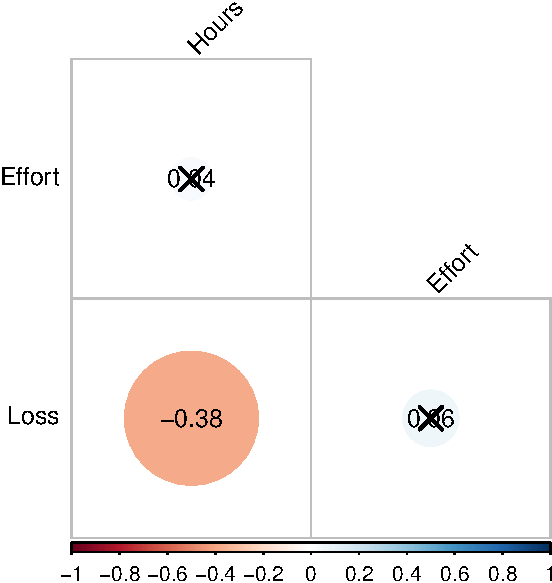
\includegraphics{Appendix_ex_weightloss_files/figure-latex/unnamed-chunk-26-1} \hfill{}

\caption{Correlation Plot for Program Time, Effort Rating, and Weight Loss, Pearson's Product Moment Correlation (r) Indication Statistical Significance, for the Reading Running}\label{fig:unnamed-chunk-26}
\end{figure}

\clearpage

\hypertarget{visualizations}{%
\section{VISUALIZATIONS}\label{visualizations}}

\hypertarget{univariable}{%
\subsection{Univariable}\label{univariable}}

\hypertarget{weight-loss}{%
\subsubsection{Weight Loss}\label{weight-loss}}

\begin{Shaded}
\begin{Highlighting}[]
\NormalTok{df\_use }\SpecialCharTok{\%\textgreater{}\%} 
  \FunctionTok{ggplot}\NormalTok{(}\FunctionTok{aes}\NormalTok{(loss)) }\SpecialCharTok{+} 
  \FunctionTok{geom\_histogram}\NormalTok{(}\AttributeTok{color =} \StringTok{"black"}\NormalTok{,}
                 \AttributeTok{alpha =}\NormalTok{ .}\DecValTok{3}\NormalTok{,}
                 \AttributeTok{binwidth =} \DecValTok{5}\NormalTok{) }\SpecialCharTok{+}
  \FunctionTok{stat\_summary}\NormalTok{(}\FunctionTok{aes}\NormalTok{(}\AttributeTok{xintercept =}\NormalTok{ ..x.., }
                   \AttributeTok{y =} \DecValTok{0}\NormalTok{), }
               \AttributeTok{fun =}\NormalTok{ mean, }
               \AttributeTok{geom =} \StringTok{"vline"}\NormalTok{, }
               \AttributeTok{orientation =} \StringTok{"y"}\NormalTok{,}
               \AttributeTok{linewidth =} \DecValTok{2}\NormalTok{) }\SpecialCharTok{+}
  \FunctionTok{labs}\NormalTok{(}\AttributeTok{x =} \StringTok{"Weight Loss, pounds"}\NormalTok{,}
       \AttributeTok{y =} \StringTok{"Count"}\NormalTok{) }\SpecialCharTok{+}
  \FunctionTok{scale\_x\_continuous}\NormalTok{(}\AttributeTok{breaks =} \FunctionTok{seq}\NormalTok{(}\AttributeTok{from =} \SpecialCharTok{{-}}\DecValTok{20}\NormalTok{, }\AttributeTok{to =} \DecValTok{50}\NormalTok{, }\AttributeTok{by =} \DecValTok{10}\NormalTok{)) }
\end{Highlighting}
\end{Shaded}

\begin{figure}[hb]

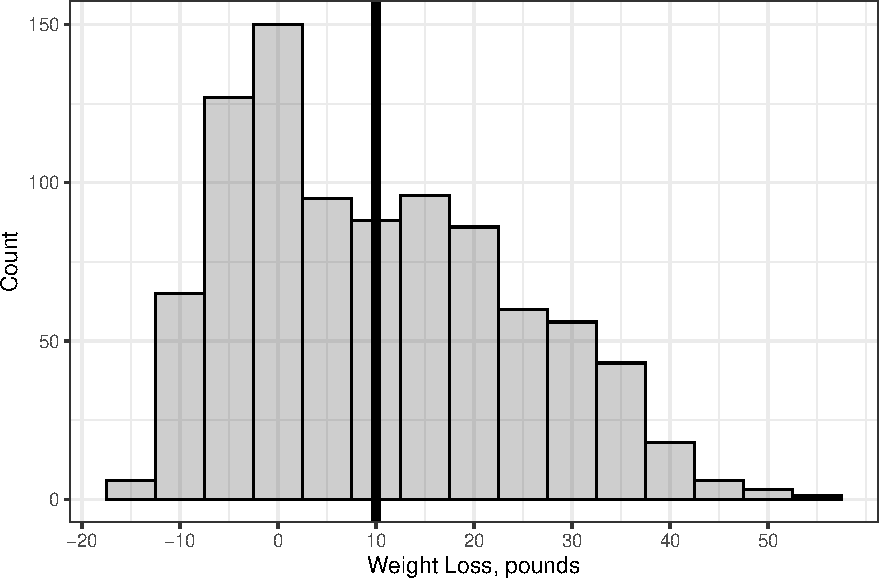
\includegraphics{Appendix_ex_weightloss_files/figure-latex/unnamed-chunk-27-1} \hfill{}

\caption{Distribution of Weight Loss}\label{fig:unnamed-chunk-27}
\end{figure}

\clearpage

\begin{Shaded}
\begin{Highlighting}[]
\NormalTok{df\_use }\SpecialCharTok{\%\textgreater{}\%} 
  \FunctionTok{ggplot}\NormalTok{(}\FunctionTok{aes}\NormalTok{(loss)) }\SpecialCharTok{+} 
  \FunctionTok{geom\_histogram}\NormalTok{(}\AttributeTok{color =} \StringTok{"black"}\NormalTok{,}
                 \AttributeTok{alpha =}\NormalTok{ .}\DecValTok{3}\NormalTok{,}
                 \AttributeTok{binwidth =} \DecValTok{5}\NormalTok{) }\SpecialCharTok{+}
  \FunctionTok{stat\_summary}\NormalTok{(}\FunctionTok{aes}\NormalTok{(}\AttributeTok{xintercept =}\NormalTok{ ..x.., }\AttributeTok{y =} \DecValTok{0}\NormalTok{),}
               \AttributeTok{fun =}\NormalTok{ mean,}
               \AttributeTok{geom =} \StringTok{"vline"}\NormalTok{,}
               \AttributeTok{orientation =} \StringTok{"y"}\NormalTok{,}
               \AttributeTok{linewidth =} \DecValTok{2}\NormalTok{) }\SpecialCharTok{+}
  \FunctionTok{labs}\NormalTok{(}\AttributeTok{x =} \StringTok{"Weight Loss, pounds"}\NormalTok{,}
       \AttributeTok{y =} \StringTok{"Count"}\NormalTok{) }\SpecialCharTok{+}
  \FunctionTok{facet\_wrap}\NormalTok{(}\SpecialCharTok{\textasciitilde{}}\NormalTok{ prog, }\AttributeTok{ncol =} \DecValTok{1}\NormalTok{) }\SpecialCharTok{+}
  \FunctionTok{geom\_vline}\NormalTok{(}\AttributeTok{xintercept =} \DecValTok{0}\NormalTok{, }\AttributeTok{color =} \StringTok{"black"}\NormalTok{, }\AttributeTok{linetype =} \StringTok{"dotted"}\NormalTok{) }\SpecialCharTok{+}
  \FunctionTok{scale\_x\_continuous}\NormalTok{(}\AttributeTok{breaks =} \FunctionTok{seq}\NormalTok{(}\AttributeTok{from =} \SpecialCharTok{{-}}\DecValTok{20}\NormalTok{, }\AttributeTok{to =} \DecValTok{50}\NormalTok{, }\AttributeTok{by =} \DecValTok{10}\NormalTok{)) }
\end{Highlighting}
\end{Shaded}

\begin{figure}[hb]

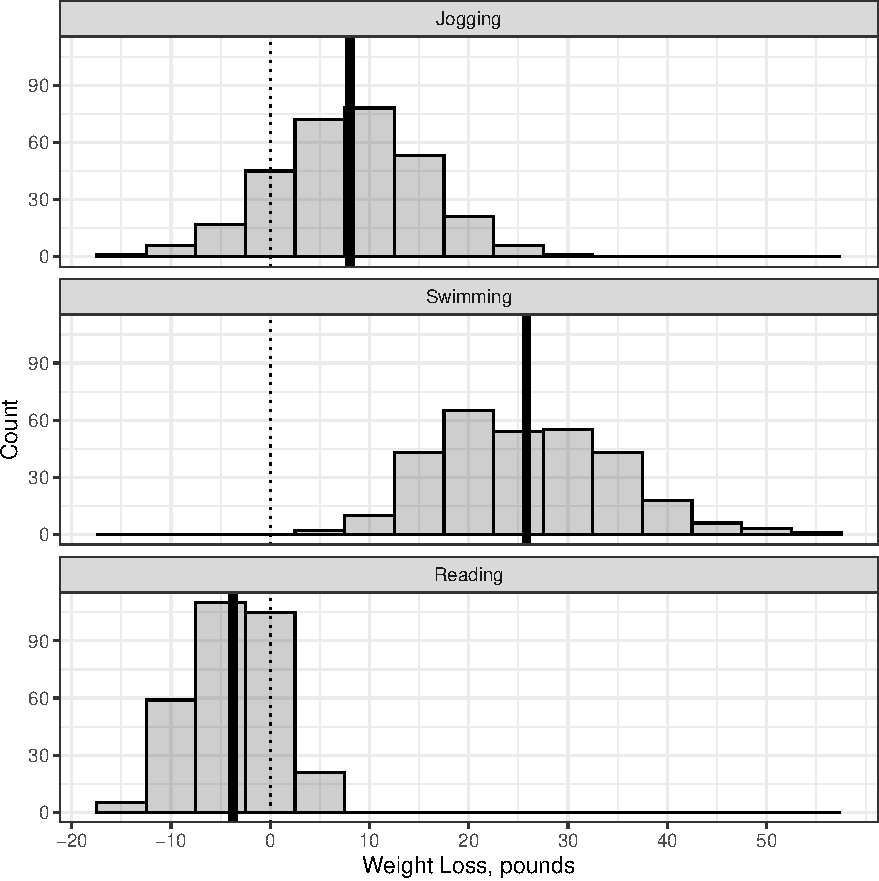
\includegraphics{Appendix_ex_weightloss_files/figure-latex/unnamed-chunk-29-1} \hfill{}

\caption{Distribution of Weight Loss, By Program - Option A}\label{fig:unnamed-chunk-29}
\end{figure}

\clearpage

\begin{Shaded}
\begin{Highlighting}[]
\NormalTok{df\_use }\SpecialCharTok{\%\textgreater{}\%} 
  \FunctionTok{ggplot}\NormalTok{(}\FunctionTok{aes}\NormalTok{(}\AttributeTok{x =}\NormalTok{ prog,}
             \AttributeTok{y =}\NormalTok{ loss)) }\SpecialCharTok{+} 
  \FunctionTok{geom\_hline}\NormalTok{(}\AttributeTok{yintercept =} \DecValTok{0}\NormalTok{, }\AttributeTok{color =} \StringTok{"black"}\NormalTok{) }\SpecialCharTok{+}
  \FunctionTok{geom\_violin}\NormalTok{(}\AttributeTok{fill =} \StringTok{"gray"}\NormalTok{) }\SpecialCharTok{+}
  \FunctionTok{geom\_boxplot}\NormalTok{(}\AttributeTok{width =}\NormalTok{ .}\DecValTok{25}\NormalTok{) }\SpecialCharTok{+}
  \FunctionTok{geom\_jitter}\NormalTok{(}\AttributeTok{size =}\NormalTok{ .}\DecValTok{75}\NormalTok{,}
              \AttributeTok{shape =} \DecValTok{1}\NormalTok{,}
              \AttributeTok{alpha =}\NormalTok{ .}\DecValTok{3}\NormalTok{,}
              \AttributeTok{width =}\NormalTok{ .}\DecValTok{2}\NormalTok{,}
              \AttributeTok{height =} \DecValTok{0}\NormalTok{) }\SpecialCharTok{+}
  \FunctionTok{stat\_summary}\NormalTok{(}\AttributeTok{fun =} \StringTok{"mean"}\NormalTok{,}
               \AttributeTok{geom =} \StringTok{"point"}\NormalTok{,}
               \AttributeTok{shape =} \DecValTok{18}\NormalTok{,}
               \AttributeTok{size =} \DecValTok{5}\NormalTok{) }\SpecialCharTok{+}
  \FunctionTok{stat\_summary}\NormalTok{(}\FunctionTok{aes}\NormalTok{(}\AttributeTok{group =} \DecValTok{1}\NormalTok{),}
               \AttributeTok{fun =} \StringTok{"mean"}\NormalTok{,}
               \AttributeTok{geom =} \StringTok{"line"}\NormalTok{) }\SpecialCharTok{+}
  \FunctionTok{labs}\NormalTok{(}\AttributeTok{x =} \StringTok{"Program, randomized"}\NormalTok{,}
       \AttributeTok{y =} \StringTok{"Weight Loss, pounds"}\NormalTok{) }\SpecialCharTok{+}
  \FunctionTok{scale\_y\_continuous}\NormalTok{(}\AttributeTok{breaks =} \FunctionTok{seq}\NormalTok{(}\AttributeTok{from =} \SpecialCharTok{{-}}\DecValTok{20}\NormalTok{, }\AttributeTok{to =} \DecValTok{50}\NormalTok{, }\AttributeTok{by =} \DecValTok{10}\NormalTok{))}
\end{Highlighting}
\end{Shaded}

\begin{figure}[hb]

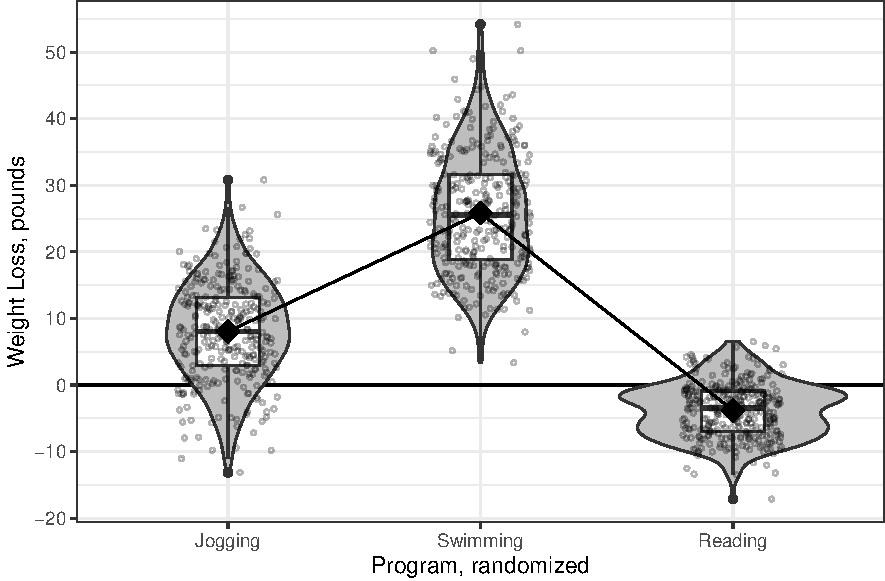
\includegraphics{Appendix_ex_weightloss_files/figure-latex/unnamed-chunk-31-1} \hfill{}

\caption{Distribution of Weight Loss, By Program - Option B}\label{fig:unnamed-chunk-31}
\end{figure}

\clearpage

\begin{Shaded}
\begin{Highlighting}[]
\NormalTok{df\_use }\SpecialCharTok{\%\textgreater{}\%} 
  \FunctionTok{ggplot}\NormalTok{(}\FunctionTok{aes}\NormalTok{(loss,}
             \AttributeTok{fill =}\NormalTok{ gender)) }\SpecialCharTok{+} 
  \FunctionTok{geom\_density}\NormalTok{(}\AttributeTok{alpha =}\NormalTok{ .}\DecValTok{5}\NormalTok{) }\SpecialCharTok{+}  
  \FunctionTok{stat\_summary}\NormalTok{(}\FunctionTok{aes}\NormalTok{(}\AttributeTok{xintercept =}\NormalTok{ ..x.., }
                   \AttributeTok{y =} \DecValTok{0}\NormalTok{,}
                   \AttributeTok{linetype =}\NormalTok{ gender), }
               \AttributeTok{fun =}\NormalTok{ mean, }
               \AttributeTok{geom =} \StringTok{"vline"}\NormalTok{, }
               \AttributeTok{orientation =} \StringTok{"y"}\NormalTok{,}
               \AttributeTok{linewidth =} \DecValTok{2}\NormalTok{) }\SpecialCharTok{+}
  \FunctionTok{geom\_vline}\NormalTok{(}\AttributeTok{xintercept =} \DecValTok{0}\NormalTok{, }
             \AttributeTok{color =} \StringTok{"black"}\NormalTok{, }
             \AttributeTok{linetype =} \StringTok{"dotted"}\NormalTok{) }\SpecialCharTok{+}
  \FunctionTok{labs}\NormalTok{(}\AttributeTok{x =} \StringTok{"Weight Loss, pounds"}\NormalTok{,}
       \AttributeTok{y =} \StringTok{"Count"}\NormalTok{,}
       \AttributeTok{fill =} \ConstantTok{NULL}\NormalTok{,}
       \AttributeTok{color =} \ConstantTok{NULL}\NormalTok{,}
       \AttributeTok{linetype =} \ConstantTok{NULL}\NormalTok{)}\SpecialCharTok{+}
  \FunctionTok{facet\_wrap}\NormalTok{(}\SpecialCharTok{\textasciitilde{}}\NormalTok{ prog, }\AttributeTok{ncol =} \DecValTok{1}\NormalTok{) }\SpecialCharTok{+}
  \FunctionTok{scale\_fill\_manual}\NormalTok{(}\AttributeTok{values =} \FunctionTok{c}\NormalTok{(}\StringTok{"gray20"}\NormalTok{, }\StringTok{"gray90"}\NormalTok{)) }\SpecialCharTok{+}
  \FunctionTok{scale\_x\_continuous}\NormalTok{(}\AttributeTok{breaks =} \FunctionTok{seq}\NormalTok{(}\AttributeTok{from =} \SpecialCharTok{{-}}\DecValTok{20}\NormalTok{, }\AttributeTok{to =} \DecValTok{50}\NormalTok{, }\AttributeTok{by =} \DecValTok{10}\NormalTok{)) }\SpecialCharTok{+}
  \FunctionTok{theme}\NormalTok{(}\AttributeTok{legend.position =} \FunctionTok{c}\NormalTok{(}\DecValTok{1}\NormalTok{, }\DecValTok{0}\NormalTok{),}
        \AttributeTok{legend.justification =} \FunctionTok{c}\NormalTok{(}\FloatTok{1.1}\NormalTok{, }\SpecialCharTok{{-}}\NormalTok{.}\DecValTok{1}\NormalTok{),}
        \AttributeTok{legend.background =} \FunctionTok{element\_rect}\NormalTok{(}\AttributeTok{color =} \StringTok{"black"}\NormalTok{),}
        \AttributeTok{legend.key.height =} \FunctionTok{unit}\NormalTok{(}\FloatTok{1.5}\NormalTok{, }\StringTok{"cm"}\NormalTok{))}
\end{Highlighting}
\end{Shaded}

\begin{figure}[hb]

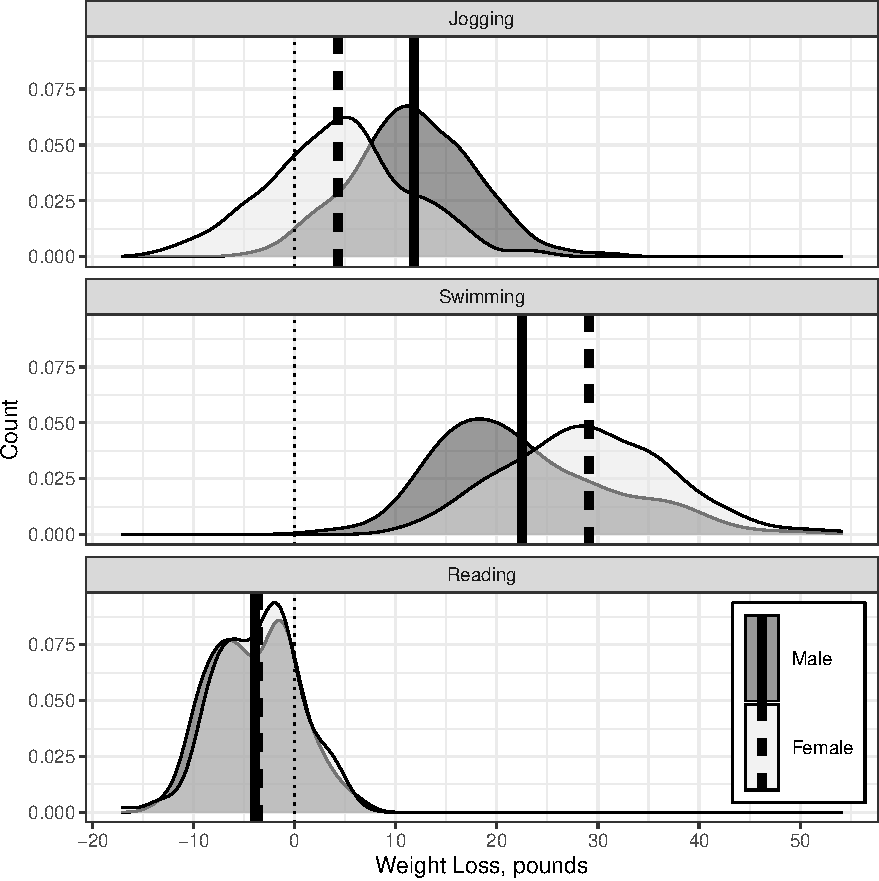
\includegraphics{Appendix_ex_weightloss_files/figure-latex/unnamed-chunk-33-1} \hfill{}

\caption{Distribution of Weight Loss, By Program and Gender - Option A}\label{fig:unnamed-chunk-33}
\end{figure}

\clearpage

\begin{Shaded}
\begin{Highlighting}[]
\NormalTok{df\_use }\SpecialCharTok{\%\textgreater{}\%} 
  \FunctionTok{ggplot}\NormalTok{(}\FunctionTok{aes}\NormalTok{(}\AttributeTok{x =}\NormalTok{ prog,}
             \AttributeTok{y =}\NormalTok{ loss,}
             \AttributeTok{fill =}\NormalTok{ gender,}
             \AttributeTok{shape =}\NormalTok{ gender,}
             \AttributeTok{group =} \FunctionTok{interaction}\NormalTok{(prog,gender))) }\SpecialCharTok{+}
  \FunctionTok{geom\_hline}\NormalTok{(}\AttributeTok{yintercept =} \DecValTok{0}\NormalTok{, }\AttributeTok{color =} \StringTok{"black"}\NormalTok{) }\SpecialCharTok{+} 
  \FunctionTok{geom\_violin}\NormalTok{(}\AttributeTok{alpha =}\NormalTok{ .}\DecValTok{5}\NormalTok{) }\SpecialCharTok{+}
  \FunctionTok{geom\_boxplot}\NormalTok{(}\AttributeTok{fill =} \StringTok{"white"}\NormalTok{,}
               \AttributeTok{width =}\NormalTok{ .}\DecValTok{25}\NormalTok{,}
               \AttributeTok{position =} \FunctionTok{position\_dodge}\NormalTok{(}\AttributeTok{width =}\NormalTok{ .}\DecValTok{9}\NormalTok{)) }\SpecialCharTok{+}
  \FunctionTok{stat\_summary}\NormalTok{(}\AttributeTok{fun =}\NormalTok{ mean,}
               \AttributeTok{geom =} \StringTok{"point"}\NormalTok{,}
               \AttributeTok{size =} \DecValTok{5}\NormalTok{,}
               \AttributeTok{position =} \FunctionTok{position\_dodge}\NormalTok{(}\AttributeTok{width =}\NormalTok{ .}\DecValTok{9}\NormalTok{)) }\SpecialCharTok{+}
  \FunctionTok{labs}\NormalTok{(}\AttributeTok{x =} \StringTok{"Program, randomized"}\NormalTok{,}
       \AttributeTok{y =} \StringTok{"Weight Loss, pounds"}\NormalTok{,}
       \AttributeTok{fill =} \ConstantTok{NULL}\NormalTok{,}
       \AttributeTok{color =} \ConstantTok{NULL}\NormalTok{,}
       \AttributeTok{shape =} \ConstantTok{NULL}\NormalTok{)  }\SpecialCharTok{+}
  \FunctionTok{scale\_fill\_manual}\NormalTok{(}\AttributeTok{values =} \FunctionTok{c}\NormalTok{(}\StringTok{"gray20"}\NormalTok{, }\StringTok{"gray90"}\NormalTok{)) }\SpecialCharTok{+}
  \FunctionTok{scale\_shape\_manual}\NormalTok{(}\AttributeTok{values =} \FunctionTok{c}\NormalTok{(}\DecValTok{18}\NormalTok{, }\DecValTok{19}\NormalTok{)) }\SpecialCharTok{+}
  \FunctionTok{scale\_y\_continuous}\NormalTok{(}\AttributeTok{breaks =} \FunctionTok{seq}\NormalTok{(}\AttributeTok{from =} \SpecialCharTok{{-}}\DecValTok{20}\NormalTok{, }\AttributeTok{to =} \DecValTok{50}\NormalTok{, }\AttributeTok{by =} \DecValTok{10}\NormalTok{)) }\SpecialCharTok{+}
  \FunctionTok{theme}\NormalTok{(}\AttributeTok{legend.position =} \FunctionTok{c}\NormalTok{(}\DecValTok{0}\NormalTok{, }\DecValTok{1}\NormalTok{),}
        \AttributeTok{legend.justification =} \FunctionTok{c}\NormalTok{(}\SpecialCharTok{{-}}\NormalTok{.}\DecValTok{1}\NormalTok{, }\FloatTok{1.1}\NormalTok{),}
        \AttributeTok{legend.background =} \FunctionTok{element\_rect}\NormalTok{(}\AttributeTok{color =} \StringTok{"black"}\NormalTok{),}
        \AttributeTok{legend.key.height =} \FunctionTok{unit}\NormalTok{(}\FloatTok{1.3}\NormalTok{, }\StringTok{"cm"}\NormalTok{),}
        \AttributeTok{legend.direction =} \StringTok{"horizontal"}\NormalTok{)}
\end{Highlighting}
\end{Shaded}

\begin{figure}[hb]

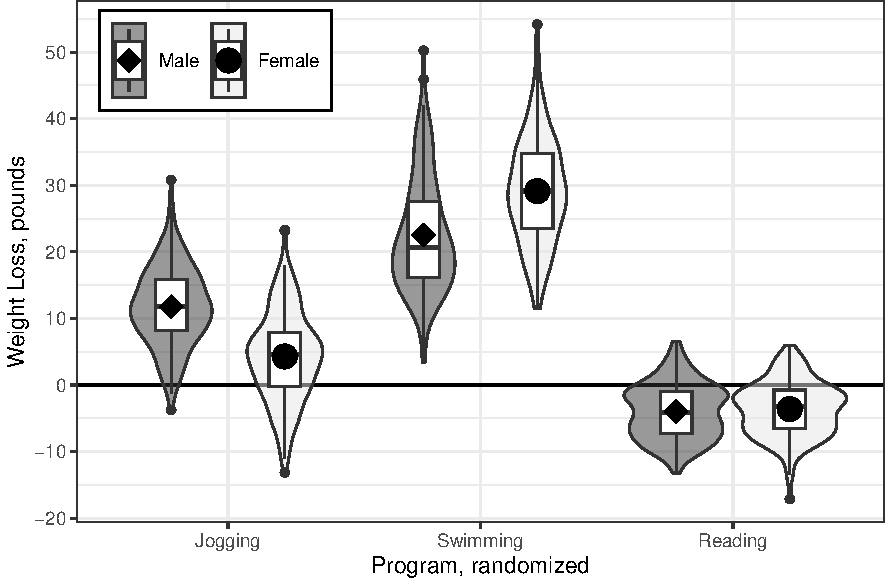
\includegraphics{Appendix_ex_weightloss_files/figure-latex/unnamed-chunk-35-1} \hfill{}

\caption{Distribution of Weight Loss, By Program and Gender - Option B}\label{fig:unnamed-chunk-35}
\end{figure}

\clearpage

\begin{Shaded}
\begin{Highlighting}[]
\NormalTok{df\_use }\SpecialCharTok{\%\textgreater{}\%} 
  \FunctionTok{ggplot}\NormalTok{(}\FunctionTok{aes}\NormalTok{(}\AttributeTok{x =}\NormalTok{ gender,}
             \AttributeTok{y =}\NormalTok{ loss,}
             \AttributeTok{shape =}\NormalTok{ gender,}
             \AttributeTok{group =}\NormalTok{ gender)) }\SpecialCharTok{+} 
  \FunctionTok{geom\_hline}\NormalTok{(}\AttributeTok{yintercept =} \DecValTok{0}\NormalTok{, }\AttributeTok{color =} \StringTok{"black"}\NormalTok{) }\SpecialCharTok{+} 
  \FunctionTok{geom\_violin}\NormalTok{(}\FunctionTok{aes}\NormalTok{(}\AttributeTok{fill =}\NormalTok{ gender),}
              \AttributeTok{alpha =}\NormalTok{ .}\DecValTok{5}\NormalTok{) }\SpecialCharTok{+}
  \FunctionTok{geom\_boxplot}\NormalTok{(}\AttributeTok{fill =} \StringTok{"white"}\NormalTok{,}
               \AttributeTok{width =}\NormalTok{ .}\DecValTok{25}\NormalTok{,}
               \AttributeTok{position =} \FunctionTok{position\_dodge}\NormalTok{(}\AttributeTok{width =}\NormalTok{ .}\DecValTok{9}\NormalTok{)) }\SpecialCharTok{+}
  \FunctionTok{stat\_summary}\NormalTok{(}\AttributeTok{fun =}\NormalTok{ mean,}
               \AttributeTok{geom =} \StringTok{"point"}\NormalTok{,}
               \AttributeTok{size =} \DecValTok{5}\NormalTok{,}
               \AttributeTok{position =} \FunctionTok{position\_dodge}\NormalTok{(}\AttributeTok{width =}\NormalTok{ .}\DecValTok{9}\NormalTok{)) }\SpecialCharTok{+}
  \FunctionTok{stat\_summary}\NormalTok{(}\FunctionTok{aes}\NormalTok{(}\AttributeTok{group =} \DecValTok{1}\NormalTok{),}
               \AttributeTok{fun =} \StringTok{"mean"}\NormalTok{,}
               \AttributeTok{geom =} \StringTok{"line"}\NormalTok{) }\SpecialCharTok{+}
  \FunctionTok{labs}\NormalTok{(}\AttributeTok{x =} \ConstantTok{NULL}\NormalTok{,}
       \AttributeTok{y =} \StringTok{"Weight Loss, pounds"}\NormalTok{,}
       \AttributeTok{shape =} \ConstantTok{NULL}\NormalTok{)  }\SpecialCharTok{+}
  \FunctionTok{scale\_shape\_manual}\NormalTok{(}\AttributeTok{values =} \FunctionTok{c}\NormalTok{(}\DecValTok{18}\NormalTok{, }\DecValTok{19}\NormalTok{)) }\SpecialCharTok{+}
  \FunctionTok{scale\_y\_continuous}\NormalTok{(}\AttributeTok{breaks =} \FunctionTok{seq}\NormalTok{(}\AttributeTok{from =} \SpecialCharTok{{-}}\DecValTok{20}\NormalTok{, }\AttributeTok{to =} \DecValTok{50}\NormalTok{, }\AttributeTok{by =} \DecValTok{10}\NormalTok{)) }\SpecialCharTok{+}
  \FunctionTok{scale\_fill\_manual}\NormalTok{(}\AttributeTok{values =} \FunctionTok{c}\NormalTok{(}\StringTok{"gray20"}\NormalTok{, }\StringTok{"gray90"}\NormalTok{)) }\SpecialCharTok{+}
  \FunctionTok{theme}\NormalTok{(}\AttributeTok{legend.position =} \StringTok{"none"}\NormalTok{) }\SpecialCharTok{+}
  \FunctionTok{facet\_grid}\NormalTok{(}\SpecialCharTok{\textasciitilde{}}\NormalTok{ prog)}
\end{Highlighting}
\end{Shaded}

\begin{figure}[hb]

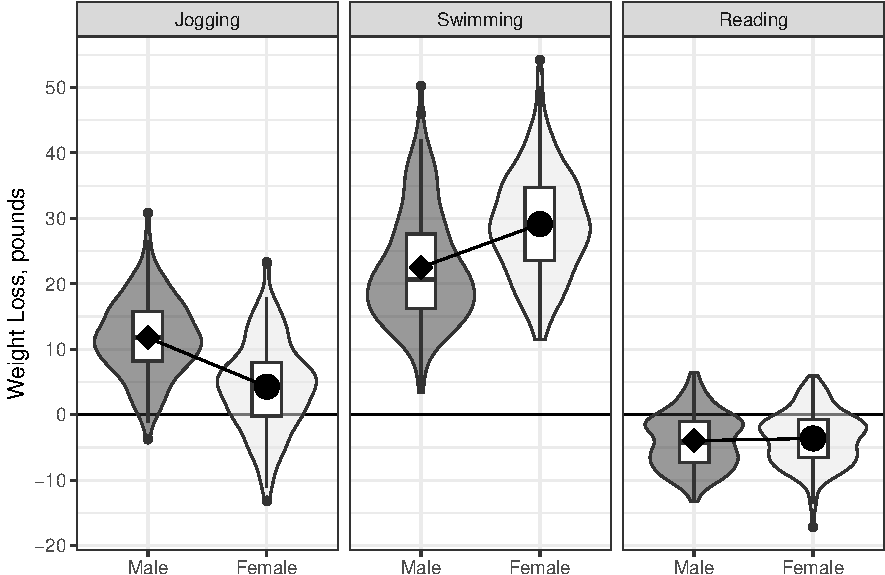
\includegraphics{Appendix_ex_weightloss_files/figure-latex/unnamed-chunk-37-1} \hfill{}

\caption{Distribution of Weight Loss, By Program and Gender - Option C}\label{fig:unnamed-chunk-37}
\end{figure}

\clearpage

\hypertarget{program-time}{%
\subsubsection{Program Time}\label{program-time}}

\begin{Shaded}
\begin{Highlighting}[]
\NormalTok{df\_use }\SpecialCharTok{\%\textgreater{}\%} 
  \FunctionTok{ggplot}\NormalTok{(}\FunctionTok{aes}\NormalTok{(hours)) }\SpecialCharTok{+} 
  \FunctionTok{geom\_histogram}\NormalTok{(}\AttributeTok{color =} \StringTok{"black"}\NormalTok{,}
                 \AttributeTok{alpha =}\NormalTok{ .}\DecValTok{3}\NormalTok{,}
                 \AttributeTok{binwidth =}\NormalTok{ .}\DecValTok{25}\NormalTok{) }\SpecialCharTok{+}
  \FunctionTok{stat\_summary}\NormalTok{(}\FunctionTok{aes}\NormalTok{(}\AttributeTok{xintercept =}\NormalTok{ ..x.., }
                   \AttributeTok{y =} \DecValTok{0}\NormalTok{), }
               \AttributeTok{fun =}\NormalTok{ mean, }
               \AttributeTok{geom =} \StringTok{"vline"}\NormalTok{, }
               \AttributeTok{orientation =} \StringTok{"y"}\NormalTok{,}
               \AttributeTok{linewidth =} \DecValTok{2}\NormalTok{) }\SpecialCharTok{+}
  \FunctionTok{labs}\NormalTok{(}\AttributeTok{x =} \StringTok{"Program Time, hours/week"}\NormalTok{,}
       \AttributeTok{y =} \StringTok{"Count"}\NormalTok{) }
\end{Highlighting}
\end{Shaded}

\begin{figure}[hb]

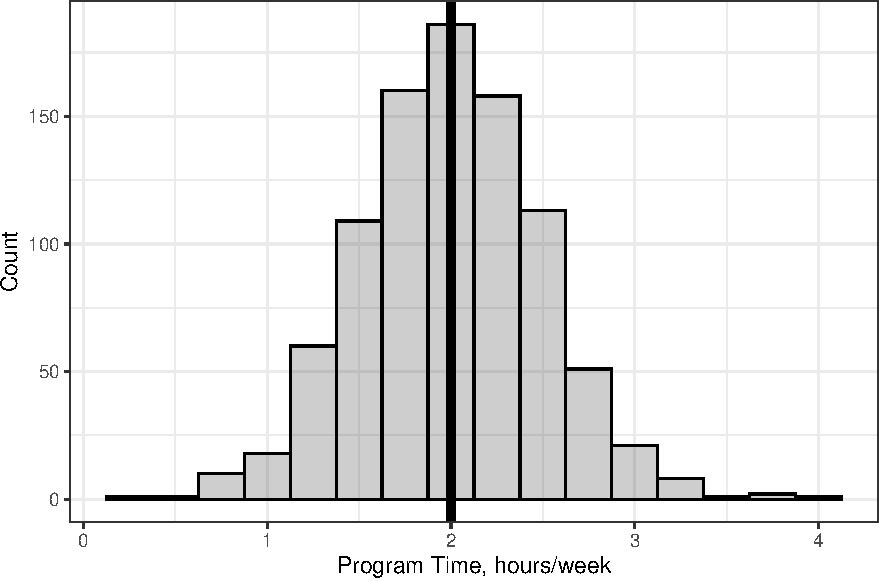
\includegraphics{Appendix_ex_weightloss_files/figure-latex/unnamed-chunk-39-1} \hfill{}

\caption{Distribution of Program Time}\label{fig:unnamed-chunk-39}
\end{figure}

\clearpage

\begin{Shaded}
\begin{Highlighting}[]
\NormalTok{df\_use }\SpecialCharTok{\%\textgreater{}\%} 
  \FunctionTok{ggplot}\NormalTok{(}\FunctionTok{aes}\NormalTok{(hours)) }\SpecialCharTok{+} 
  \FunctionTok{geom\_histogram}\NormalTok{(}\AttributeTok{color =} \StringTok{"black"}\NormalTok{,}
                 \AttributeTok{alpha =}\NormalTok{ .}\DecValTok{3}\NormalTok{,}
                 \AttributeTok{binwidth =}\NormalTok{ .}\DecValTok{25}\NormalTok{) }\SpecialCharTok{+}
  \FunctionTok{stat\_summary}\NormalTok{(}\FunctionTok{aes}\NormalTok{(}\AttributeTok{xintercept =}\NormalTok{ ..x.., }\AttributeTok{y =} \DecValTok{0}\NormalTok{),}
               \AttributeTok{fun =}\NormalTok{ mean,}
               \AttributeTok{geom =} \StringTok{"vline"}\NormalTok{,}
               \AttributeTok{orientation =} \StringTok{"y"}\NormalTok{,}
               \AttributeTok{linewidth =} \DecValTok{2}\NormalTok{) }\SpecialCharTok{+}
  \FunctionTok{labs}\NormalTok{(}\AttributeTok{x =} \StringTok{"Program Time, hours/week"}\NormalTok{,}
       \AttributeTok{y =} \StringTok{"Count"}\NormalTok{) }\SpecialCharTok{+}
  \FunctionTok{facet\_wrap}\NormalTok{(}\SpecialCharTok{\textasciitilde{}}\NormalTok{ prog, }\AttributeTok{ncol =} \DecValTok{1}\NormalTok{)}
\end{Highlighting}
\end{Shaded}

\begin{figure}[hb]

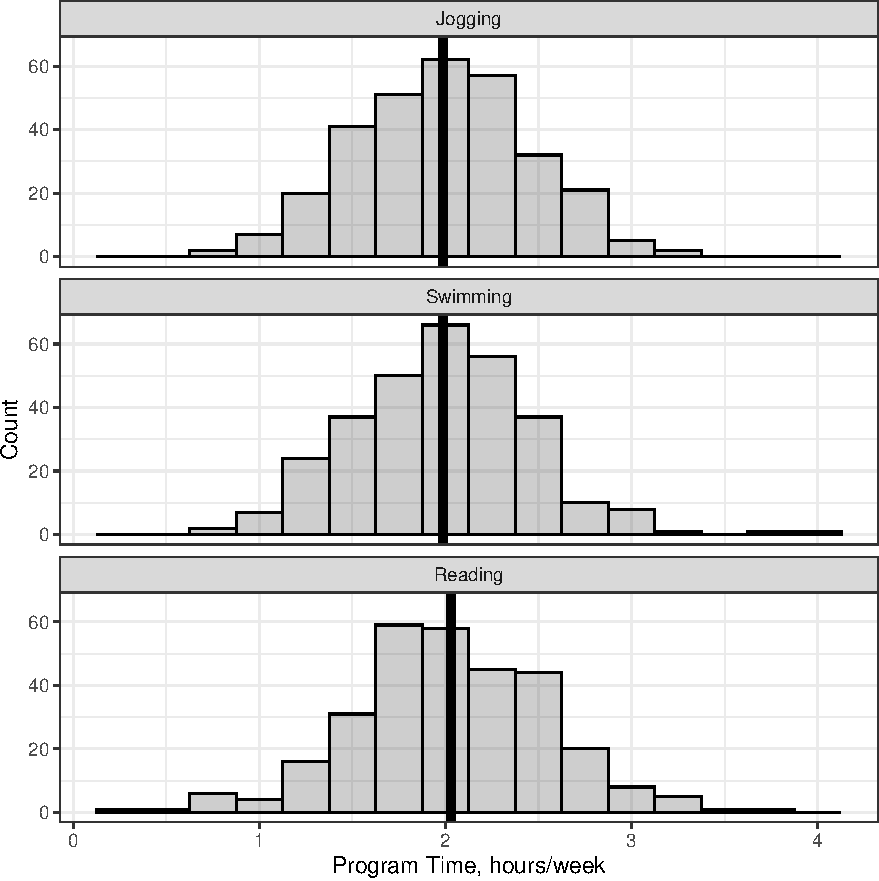
\includegraphics{Appendix_ex_weightloss_files/figure-latex/unnamed-chunk-41-1} \hfill{}

\caption{Distribution of Program Time, By Program - Option A}\label{fig:unnamed-chunk-41}
\end{figure}

\clearpage

\begin{Shaded}
\begin{Highlighting}[]
\NormalTok{df\_use }\SpecialCharTok{\%\textgreater{}\%} 
  \FunctionTok{ggplot}\NormalTok{(}\FunctionTok{aes}\NormalTok{(}\AttributeTok{x =}\NormalTok{ prog,}
             \AttributeTok{y =}\NormalTok{ hours)) }\SpecialCharTok{+} 
  \FunctionTok{geom\_violin}\NormalTok{(}\AttributeTok{fill =} \StringTok{"gray"}\NormalTok{) }\SpecialCharTok{+}
  \FunctionTok{geom\_boxplot}\NormalTok{(}\AttributeTok{width =}\NormalTok{ .}\DecValTok{25}\NormalTok{) }\SpecialCharTok{+}
  \FunctionTok{geom\_jitter}\NormalTok{(}\AttributeTok{size =}\NormalTok{ .}\DecValTok{75}\NormalTok{,}
              \AttributeTok{shape =} \DecValTok{1}\NormalTok{,}
              \AttributeTok{alpha =}\NormalTok{ .}\DecValTok{3}\NormalTok{,}
              \AttributeTok{width =}\NormalTok{ .}\DecValTok{2}\NormalTok{,}
              \AttributeTok{height =} \DecValTok{0}\NormalTok{) }\SpecialCharTok{+}
  \FunctionTok{stat\_summary}\NormalTok{(}\AttributeTok{fun =} \StringTok{"mean"}\NormalTok{,}
               \AttributeTok{geom =} \StringTok{"point"}\NormalTok{,}
               \AttributeTok{shape =} \DecValTok{18}\NormalTok{,}
               \AttributeTok{size =} \DecValTok{5}\NormalTok{) }\SpecialCharTok{+}
  \FunctionTok{stat\_summary}\NormalTok{(}\FunctionTok{aes}\NormalTok{(}\AttributeTok{group =} \DecValTok{1}\NormalTok{),}
               \AttributeTok{fun =} \StringTok{"mean"}\NormalTok{,}
               \AttributeTok{geom =} \StringTok{"line"}\NormalTok{) }\SpecialCharTok{+}
  \FunctionTok{labs}\NormalTok{(}\AttributeTok{x =} \StringTok{"Program, randomized"}\NormalTok{,}
       \AttributeTok{y =} \StringTok{"Program Time, hours/week"}\NormalTok{) }
\end{Highlighting}
\end{Shaded}

\begin{figure}[hb]

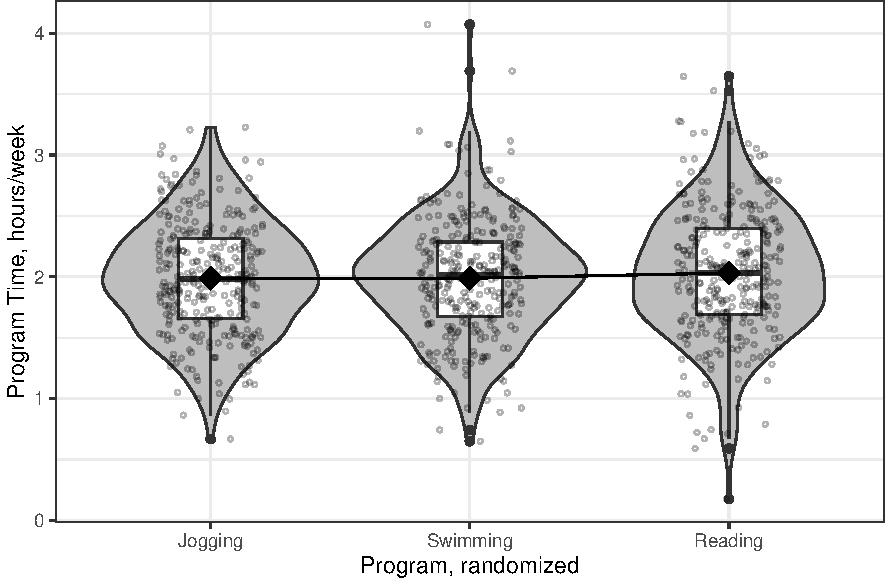
\includegraphics{Appendix_ex_weightloss_files/figure-latex/unnamed-chunk-43-1} \hfill{}

\caption{Distribution of Program Time, By Program - Option B}\label{fig:unnamed-chunk-43}
\end{figure}

\clearpage

\begin{Shaded}
\begin{Highlighting}[]
\NormalTok{df\_use }\SpecialCharTok{\%\textgreater{}\%} 
  \FunctionTok{ggplot}\NormalTok{(}\FunctionTok{aes}\NormalTok{(hours,}
             \AttributeTok{fill =}\NormalTok{ gender)) }\SpecialCharTok{+} 
  \FunctionTok{geom\_density}\NormalTok{(}\AttributeTok{alpha =}\NormalTok{ .}\DecValTok{5}\NormalTok{) }\SpecialCharTok{+}  
  \FunctionTok{stat\_summary}\NormalTok{(}\FunctionTok{aes}\NormalTok{(}\AttributeTok{xintercept =}\NormalTok{ ..x.., }
                   \AttributeTok{y =} \DecValTok{0}\NormalTok{,}
                   \AttributeTok{linetype =}\NormalTok{ gender), }
               \AttributeTok{fun =}\NormalTok{ mean, }
               \AttributeTok{geom =} \StringTok{"vline"}\NormalTok{, }
               \AttributeTok{orientation =} \StringTok{"y"}\NormalTok{,}
               \AttributeTok{linewidth =} \DecValTok{2}\NormalTok{) }\SpecialCharTok{+}
  \FunctionTok{labs}\NormalTok{(}\AttributeTok{x =} \StringTok{"Program Time, hours/week"}\NormalTok{,}
       \AttributeTok{y =} \StringTok{"Count"}\NormalTok{,}
       \AttributeTok{fill =} \ConstantTok{NULL}\NormalTok{,}
       \AttributeTok{color =} \ConstantTok{NULL}\NormalTok{,}
       \AttributeTok{linetype =} \ConstantTok{NULL}\NormalTok{)}\SpecialCharTok{+}
  \FunctionTok{facet\_wrap}\NormalTok{(}\SpecialCharTok{\textasciitilde{}}\NormalTok{ prog, }\AttributeTok{ncol =} \DecValTok{1}\NormalTok{) }\SpecialCharTok{+}
  \FunctionTok{scale\_fill\_manual}\NormalTok{(}\AttributeTok{values =} \FunctionTok{c}\NormalTok{(}\StringTok{"gray20"}\NormalTok{, }\StringTok{"gray90"}\NormalTok{)) }\SpecialCharTok{+}
  \FunctionTok{theme}\NormalTok{(}\AttributeTok{legend.position =} \FunctionTok{c}\NormalTok{(}\DecValTok{1}\NormalTok{, }\DecValTok{0}\NormalTok{),}
        \AttributeTok{legend.justification =} \FunctionTok{c}\NormalTok{(}\FloatTok{1.1}\NormalTok{, }\SpecialCharTok{{-}}\NormalTok{.}\DecValTok{1}\NormalTok{),}
        \AttributeTok{legend.background =} \FunctionTok{element\_rect}\NormalTok{(}\AttributeTok{color =} \StringTok{"black"}\NormalTok{),}
        \AttributeTok{legend.key.height =} \FunctionTok{unit}\NormalTok{(}\FloatTok{1.5}\NormalTok{, }\StringTok{"cm"}\NormalTok{))}
\end{Highlighting}
\end{Shaded}

\begin{figure}[hb]

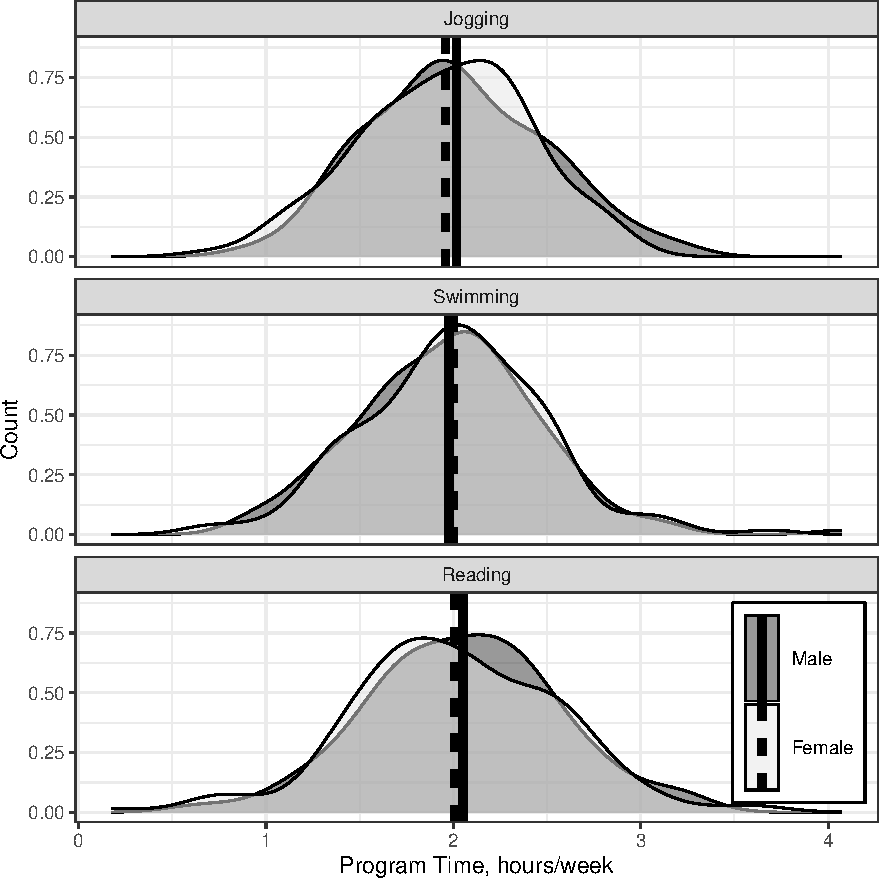
\includegraphics{Appendix_ex_weightloss_files/figure-latex/unnamed-chunk-45-1} \hfill{}

\caption{Distribution of Program Time, By Program and Gender - Option A}\label{fig:unnamed-chunk-45}
\end{figure}

\clearpage

\begin{Shaded}
\begin{Highlighting}[]
\NormalTok{df\_use }\SpecialCharTok{\%\textgreater{}\%} 
  \FunctionTok{ggplot}\NormalTok{(}\FunctionTok{aes}\NormalTok{(}\AttributeTok{x =}\NormalTok{ prog,}
             \AttributeTok{y =}\NormalTok{ hours,}
             \AttributeTok{fill =}\NormalTok{ gender,}
             \AttributeTok{shape =}\NormalTok{ gender,}
             \AttributeTok{group =} \FunctionTok{interaction}\NormalTok{(prog,gender))) }\SpecialCharTok{+} 
  \FunctionTok{geom\_violin}\NormalTok{(}\AttributeTok{alpha =}\NormalTok{ .}\DecValTok{5}\NormalTok{) }\SpecialCharTok{+}
  \FunctionTok{geom\_boxplot}\NormalTok{(}\AttributeTok{fill =} \StringTok{"white"}\NormalTok{,}
               \AttributeTok{width =}\NormalTok{ .}\DecValTok{25}\NormalTok{,}
               \AttributeTok{position =} \FunctionTok{position\_dodge}\NormalTok{(}\AttributeTok{width =}\NormalTok{ .}\DecValTok{9}\NormalTok{)) }\SpecialCharTok{+}
  \FunctionTok{stat\_summary}\NormalTok{(}\AttributeTok{fun =}\NormalTok{ mean,}
               \AttributeTok{geom =} \StringTok{"point"}\NormalTok{,}
               \AttributeTok{size =} \DecValTok{5}\NormalTok{,}
               \AttributeTok{position =} \FunctionTok{position\_dodge}\NormalTok{(}\AttributeTok{width =}\NormalTok{ .}\DecValTok{9}\NormalTok{)) }\SpecialCharTok{+}
  \FunctionTok{labs}\NormalTok{(}\AttributeTok{x =} \StringTok{"Program, randomized"}\NormalTok{,}
       \AttributeTok{y =} \StringTok{"Program Time, hours/week"}\NormalTok{,}
       \AttributeTok{fill =} \ConstantTok{NULL}\NormalTok{,}
       \AttributeTok{color =} \ConstantTok{NULL}\NormalTok{,}
       \AttributeTok{shape =} \ConstantTok{NULL}\NormalTok{)  }\SpecialCharTok{+}
  \FunctionTok{scale\_fill\_manual}\NormalTok{(}\AttributeTok{values =} \FunctionTok{c}\NormalTok{(}\StringTok{"gray20"}\NormalTok{, }\StringTok{"gray90"}\NormalTok{)) }\SpecialCharTok{+}
  \FunctionTok{scale\_shape\_manual}\NormalTok{(}\AttributeTok{values =} \FunctionTok{c}\NormalTok{(}\DecValTok{18}\NormalTok{, }\DecValTok{19}\NormalTok{)) }\SpecialCharTok{+}
  \FunctionTok{theme}\NormalTok{(}\AttributeTok{legend.position =} \FunctionTok{c}\NormalTok{(}\DecValTok{0}\NormalTok{, }\DecValTok{1}\NormalTok{),}
        \AttributeTok{legend.justification =} \FunctionTok{c}\NormalTok{(}\SpecialCharTok{{-}}\NormalTok{.}\DecValTok{1}\NormalTok{, }\FloatTok{1.1}\NormalTok{),}
        \AttributeTok{legend.background =} \FunctionTok{element\_rect}\NormalTok{(}\AttributeTok{color =} \StringTok{"black"}\NormalTok{),}
        \AttributeTok{legend.key.height =} \FunctionTok{unit}\NormalTok{(}\FloatTok{1.3}\NormalTok{, }\StringTok{"cm"}\NormalTok{),}
        \AttributeTok{legend.direction =} \StringTok{"horizontal"}\NormalTok{)}
\end{Highlighting}
\end{Shaded}

\begin{figure}[hb]

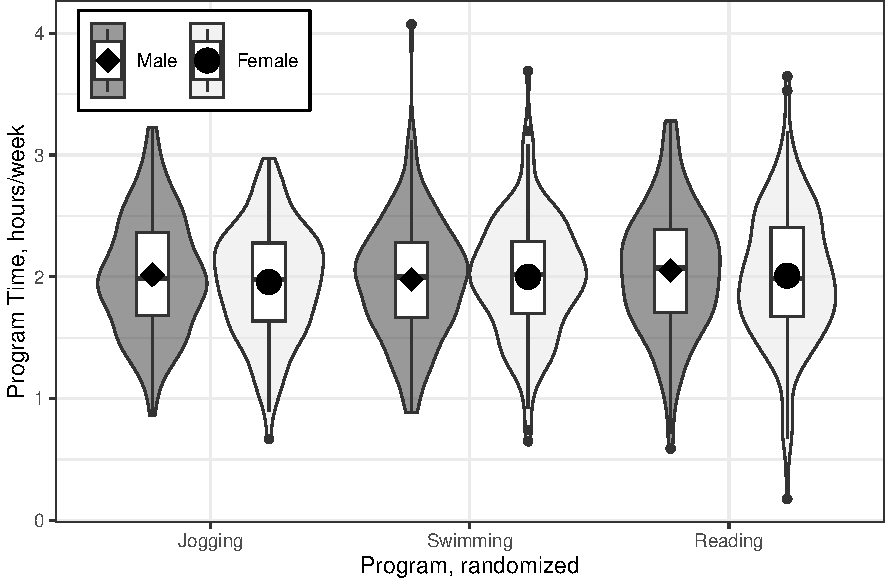
\includegraphics{Appendix_ex_weightloss_files/figure-latex/unnamed-chunk-47-1} \hfill{}

\caption{Distribution of Program Time, By Program and Gender - Option B}\label{fig:unnamed-chunk-47}
\end{figure}

\clearpage

\begin{Shaded}
\begin{Highlighting}[]
\NormalTok{df\_use }\SpecialCharTok{\%\textgreater{}\%} 
  \FunctionTok{ggplot}\NormalTok{(}\FunctionTok{aes}\NormalTok{(}\AttributeTok{x =}\NormalTok{ gender,}
             \AttributeTok{y =}\NormalTok{ hours,}
             \AttributeTok{shape =}\NormalTok{ gender,}
             \AttributeTok{group =}\NormalTok{ gender)) }\SpecialCharTok{+} 
  \FunctionTok{geom\_violin}\NormalTok{(}\FunctionTok{aes}\NormalTok{(}\AttributeTok{fill =}\NormalTok{ gender),}
              \AttributeTok{alpha =}\NormalTok{ .}\DecValTok{5}\NormalTok{) }\SpecialCharTok{+}
  \FunctionTok{geom\_boxplot}\NormalTok{(}\AttributeTok{fill =} \StringTok{"white"}\NormalTok{,}
               \AttributeTok{width =}\NormalTok{ .}\DecValTok{25}\NormalTok{,}
               \AttributeTok{position =} \FunctionTok{position\_dodge}\NormalTok{(}\AttributeTok{width =}\NormalTok{ .}\DecValTok{9}\NormalTok{)) }\SpecialCharTok{+}
  \FunctionTok{stat\_summary}\NormalTok{(}\AttributeTok{fun =}\NormalTok{ mean,}
               \AttributeTok{geom =} \StringTok{"point"}\NormalTok{,}
               \AttributeTok{size =} \DecValTok{5}\NormalTok{,}
               \AttributeTok{position =} \FunctionTok{position\_dodge}\NormalTok{(}\AttributeTok{width =}\NormalTok{ .}\DecValTok{9}\NormalTok{)) }\SpecialCharTok{+}
  \FunctionTok{stat\_summary}\NormalTok{(}\FunctionTok{aes}\NormalTok{(}\AttributeTok{group =} \DecValTok{1}\NormalTok{),}
               \AttributeTok{fun =} \StringTok{"mean"}\NormalTok{,}
               \AttributeTok{geom =} \StringTok{"line"}\NormalTok{) }\SpecialCharTok{+}
  \FunctionTok{scale\_fill\_manual}\NormalTok{(}\AttributeTok{values =} \FunctionTok{c}\NormalTok{(}\StringTok{"gray20"}\NormalTok{, }\StringTok{"gray90"}\NormalTok{)) }\SpecialCharTok{+}
  \FunctionTok{labs}\NormalTok{(}\AttributeTok{x =} \ConstantTok{NULL}\NormalTok{,}
       \AttributeTok{y =} \StringTok{"Program Time, hours/week"}\NormalTok{,}
       \AttributeTok{shape =} \ConstantTok{NULL}\NormalTok{)  }\SpecialCharTok{+}
  \FunctionTok{scale\_shape\_manual}\NormalTok{(}\AttributeTok{values =} \FunctionTok{c}\NormalTok{(}\DecValTok{18}\NormalTok{, }\DecValTok{19}\NormalTok{)) }\SpecialCharTok{+}
  \FunctionTok{theme}\NormalTok{(}\AttributeTok{legend.position =} \StringTok{"none"}\NormalTok{) }\SpecialCharTok{+}
  \FunctionTok{facet\_grid}\NormalTok{(}\SpecialCharTok{\textasciitilde{}}\NormalTok{ prog)}
\end{Highlighting}
\end{Shaded}

\begin{figure}[hb]

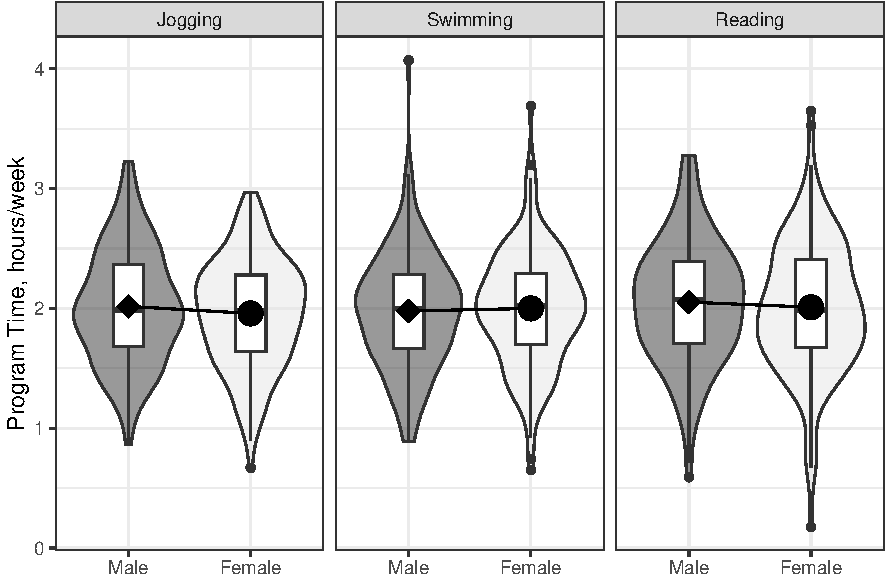
\includegraphics{Appendix_ex_weightloss_files/figure-latex/unnamed-chunk-49-1} \hfill{}

\caption{Distribution of Program Time, By Program and Gender - Option C}\label{fig:unnamed-chunk-49}
\end{figure}

\clearpage

\hypertarget{effort-rating}{%
\subsubsection{Effort Rating}\label{effort-rating}}

\begin{Shaded}
\begin{Highlighting}[]
\NormalTok{df\_use }\SpecialCharTok{\%\textgreater{}\%} 
  \FunctionTok{ggplot}\NormalTok{(}\FunctionTok{aes}\NormalTok{(effort)) }\SpecialCharTok{+} 
  \FunctionTok{geom\_histogram}\NormalTok{(}\AttributeTok{color =} \StringTok{"black"}\NormalTok{,}
                 \AttributeTok{alpha =}\NormalTok{ .}\DecValTok{3}\NormalTok{,}
                 \AttributeTok{binwidth =} \DecValTok{2}\NormalTok{) }\SpecialCharTok{+}
  \FunctionTok{stat\_summary}\NormalTok{(}\FunctionTok{aes}\NormalTok{(}\AttributeTok{xintercept =}\NormalTok{ ..x.., }
                   \AttributeTok{y =} \DecValTok{0}\NormalTok{), }
               \AttributeTok{fun =}\NormalTok{ mean, }
               \AttributeTok{geom =} \StringTok{"vline"}\NormalTok{, }
               \AttributeTok{orientation =} \StringTok{"y"}\NormalTok{,}
               \AttributeTok{linewidth =} \DecValTok{2}\NormalTok{) }\SpecialCharTok{+}
  \FunctionTok{labs}\NormalTok{(}\AttributeTok{x =} \StringTok{"Effort Rating, 0{-}50"}\NormalTok{,}
       \AttributeTok{y =} \StringTok{"Count"}\NormalTok{)}
\end{Highlighting}
\end{Shaded}

\begin{figure}[hb]

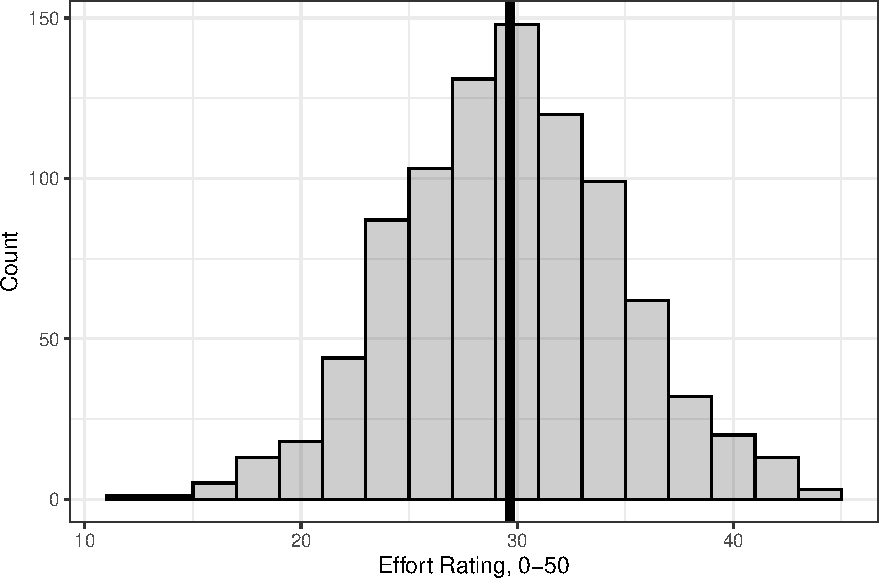
\includegraphics{Appendix_ex_weightloss_files/figure-latex/unnamed-chunk-51-1} \hfill{}

\caption{Distribution of Effort Rating}\label{fig:unnamed-chunk-51}
\end{figure}

\clearpage

\begin{Shaded}
\begin{Highlighting}[]
\NormalTok{df\_use }\SpecialCharTok{\%\textgreater{}\%} 
  \FunctionTok{ggplot}\NormalTok{(}\FunctionTok{aes}\NormalTok{(effort)) }\SpecialCharTok{+} 
  \FunctionTok{geom\_histogram}\NormalTok{(}\AttributeTok{color =} \StringTok{"black"}\NormalTok{,}
                 \AttributeTok{alpha =}\NormalTok{ .}\DecValTok{3}\NormalTok{,}
                 \AttributeTok{binwidth =} \DecValTok{2}\NormalTok{) }\SpecialCharTok{+}
  \FunctionTok{stat\_summary}\NormalTok{(}\FunctionTok{aes}\NormalTok{(}\AttributeTok{xintercept =}\NormalTok{ ..x.., }\AttributeTok{y =} \DecValTok{0}\NormalTok{),}
               \AttributeTok{fun =}\NormalTok{ mean,}
               \AttributeTok{geom =} \StringTok{"vline"}\NormalTok{,}
               \AttributeTok{orientation =} \StringTok{"y"}\NormalTok{,}
               \AttributeTok{linewidth =} \DecValTok{2}\NormalTok{) }\SpecialCharTok{+}
  \FunctionTok{labs}\NormalTok{(}\AttributeTok{x =} \StringTok{"Effort Rating, 0{-}50"}\NormalTok{,}
       \AttributeTok{y =} \StringTok{"Count"}\NormalTok{) }\SpecialCharTok{+}
  \FunctionTok{facet\_wrap}\NormalTok{(}\SpecialCharTok{\textasciitilde{}}\NormalTok{ prog, }\AttributeTok{ncol =} \DecValTok{1}\NormalTok{)}
\end{Highlighting}
\end{Shaded}

\begin{figure}[hb]

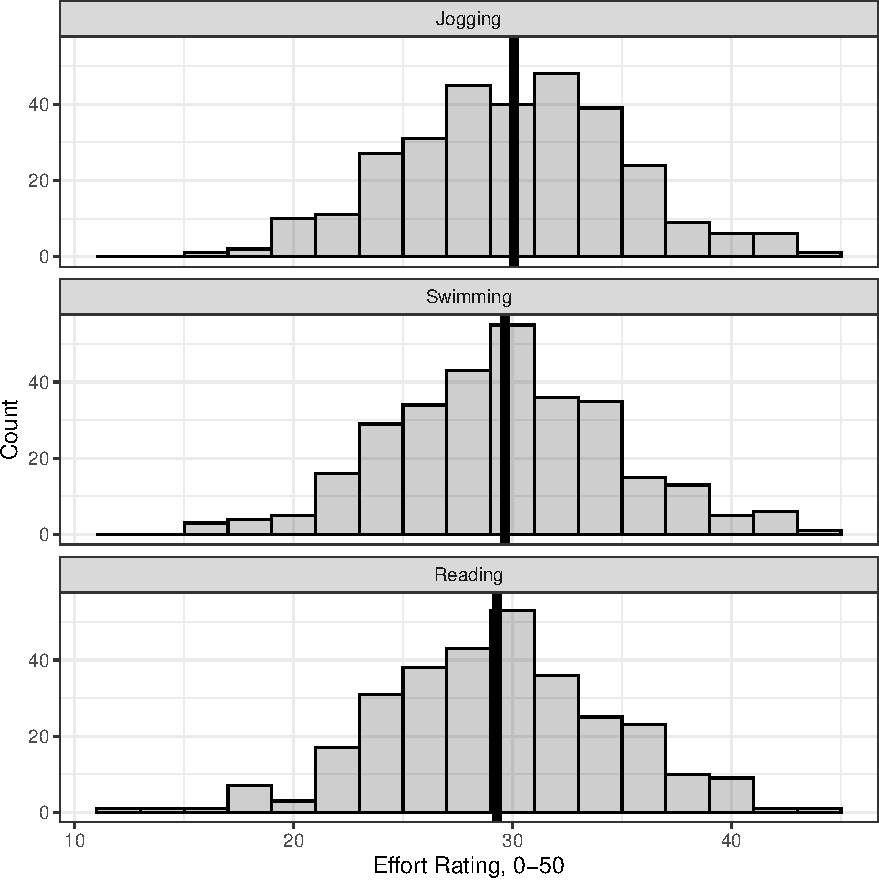
\includegraphics{Appendix_ex_weightloss_files/figure-latex/unnamed-chunk-53-1} \hfill{}

\caption{Distribution of Effort Rating, By Program - Option A}\label{fig:unnamed-chunk-53}
\end{figure}

\clearpage

\begin{Shaded}
\begin{Highlighting}[]
\NormalTok{df\_use }\SpecialCharTok{\%\textgreater{}\%} 
  \FunctionTok{ggplot}\NormalTok{(}\FunctionTok{aes}\NormalTok{(}\AttributeTok{x =}\NormalTok{ prog,}
             \AttributeTok{y =}\NormalTok{ effort)) }\SpecialCharTok{+} 
  \FunctionTok{geom\_violin}\NormalTok{(}\AttributeTok{fill =} \StringTok{"gray"}\NormalTok{) }\SpecialCharTok{+}
  \FunctionTok{geom\_boxplot}\NormalTok{(}\AttributeTok{width =}\NormalTok{ .}\DecValTok{25}\NormalTok{) }\SpecialCharTok{+}
  \FunctionTok{geom\_jitter}\NormalTok{(}\AttributeTok{size =}\NormalTok{ .}\DecValTok{75}\NormalTok{,}
              \AttributeTok{shape =} \DecValTok{1}\NormalTok{,}
              \AttributeTok{alpha =}\NormalTok{ .}\DecValTok{3}\NormalTok{,}
              \AttributeTok{width =}\NormalTok{ .}\DecValTok{2}\NormalTok{,}
              \AttributeTok{height =} \DecValTok{0}\NormalTok{) }\SpecialCharTok{+}
  \FunctionTok{stat\_summary}\NormalTok{(}\AttributeTok{fun =} \StringTok{"mean"}\NormalTok{,}
               \AttributeTok{geom =} \StringTok{"point"}\NormalTok{,}
               \AttributeTok{shape =} \DecValTok{18}\NormalTok{,}
               \AttributeTok{size =} \DecValTok{5}\NormalTok{) }\SpecialCharTok{+}
  \FunctionTok{stat\_summary}\NormalTok{(}\FunctionTok{aes}\NormalTok{(}\AttributeTok{group =} \DecValTok{1}\NormalTok{),}
               \AttributeTok{fun =} \StringTok{"mean"}\NormalTok{,}
               \AttributeTok{geom =} \StringTok{"line"}\NormalTok{) }\SpecialCharTok{+}
  \FunctionTok{labs}\NormalTok{(}\AttributeTok{x =} \StringTok{"Program, randomized"}\NormalTok{,}
       \AttributeTok{y =} \StringTok{"Effort Rating, 0{-}50"}\NormalTok{) }
\end{Highlighting}
\end{Shaded}

\begin{figure}[hb]

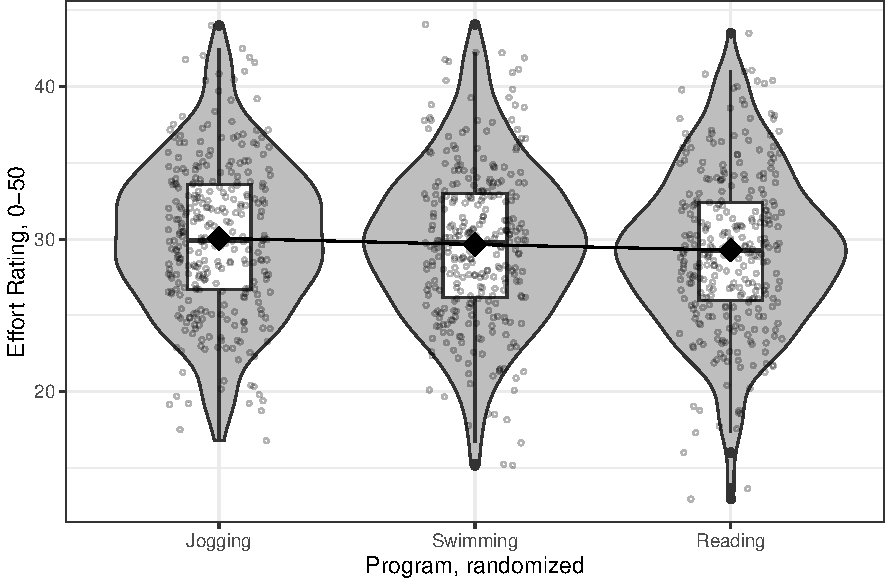
\includegraphics{Appendix_ex_weightloss_files/figure-latex/unnamed-chunk-55-1} \hfill{}

\caption{Distribution of Effort Rating, By Program - Option B}\label{fig:unnamed-chunk-55}
\end{figure}

\clearpage

\begin{Shaded}
\begin{Highlighting}[]
\NormalTok{df\_use }\SpecialCharTok{\%\textgreater{}\%} 
  \FunctionTok{ggplot}\NormalTok{(}\FunctionTok{aes}\NormalTok{(effort,}
             \AttributeTok{fill =}\NormalTok{ gender)) }\SpecialCharTok{+} 
  \FunctionTok{geom\_density}\NormalTok{(}\AttributeTok{alpha =}\NormalTok{ .}\DecValTok{5}\NormalTok{) }\SpecialCharTok{+}  
  \FunctionTok{stat\_summary}\NormalTok{(}\FunctionTok{aes}\NormalTok{(}\AttributeTok{xintercept =}\NormalTok{ ..x.., }
                   \AttributeTok{y =} \DecValTok{0}\NormalTok{,}
                   \AttributeTok{linetype =}\NormalTok{ gender), }
               \AttributeTok{fun =}\NormalTok{ mean, }
               \AttributeTok{geom =} \StringTok{"vline"}\NormalTok{, }
               \AttributeTok{orientation =} \StringTok{"y"}\NormalTok{,}
               \AttributeTok{linewidth =} \DecValTok{2}\NormalTok{) }\SpecialCharTok{+}
  \FunctionTok{labs}\NormalTok{(}\AttributeTok{x =} \StringTok{"Effort Rating, 0{-}50"}\NormalTok{,}
       \AttributeTok{y =} \StringTok{"Count"}\NormalTok{,}
       \AttributeTok{fill =} \ConstantTok{NULL}\NormalTok{,}
       \AttributeTok{linetype =} \ConstantTok{NULL}\NormalTok{)}\SpecialCharTok{+}
  \FunctionTok{facet\_wrap}\NormalTok{(}\SpecialCharTok{\textasciitilde{}}\NormalTok{ prog, }\AttributeTok{ncol =} \DecValTok{1}\NormalTok{) }\SpecialCharTok{+}
  \FunctionTok{scale\_fill\_manual}\NormalTok{(}\AttributeTok{values =} \FunctionTok{c}\NormalTok{(}\StringTok{"gray20"}\NormalTok{, }\StringTok{"gray90"}\NormalTok{)) }\SpecialCharTok{+}
  \FunctionTok{theme}\NormalTok{(}\AttributeTok{legend.position =} \FunctionTok{c}\NormalTok{(}\DecValTok{1}\NormalTok{, }\DecValTok{0}\NormalTok{),}
        \AttributeTok{legend.justification =} \FunctionTok{c}\NormalTok{(}\FloatTok{1.1}\NormalTok{, }\SpecialCharTok{{-}}\NormalTok{.}\DecValTok{1}\NormalTok{),}
        \AttributeTok{legend.background =} \FunctionTok{element\_rect}\NormalTok{(}\AttributeTok{color =} \StringTok{"black"}\NormalTok{),}
        \AttributeTok{legend.key.height =} \FunctionTok{unit}\NormalTok{(}\FloatTok{1.5}\NormalTok{, }\StringTok{"cm"}\NormalTok{))}
\end{Highlighting}
\end{Shaded}

\begin{figure}[hb]

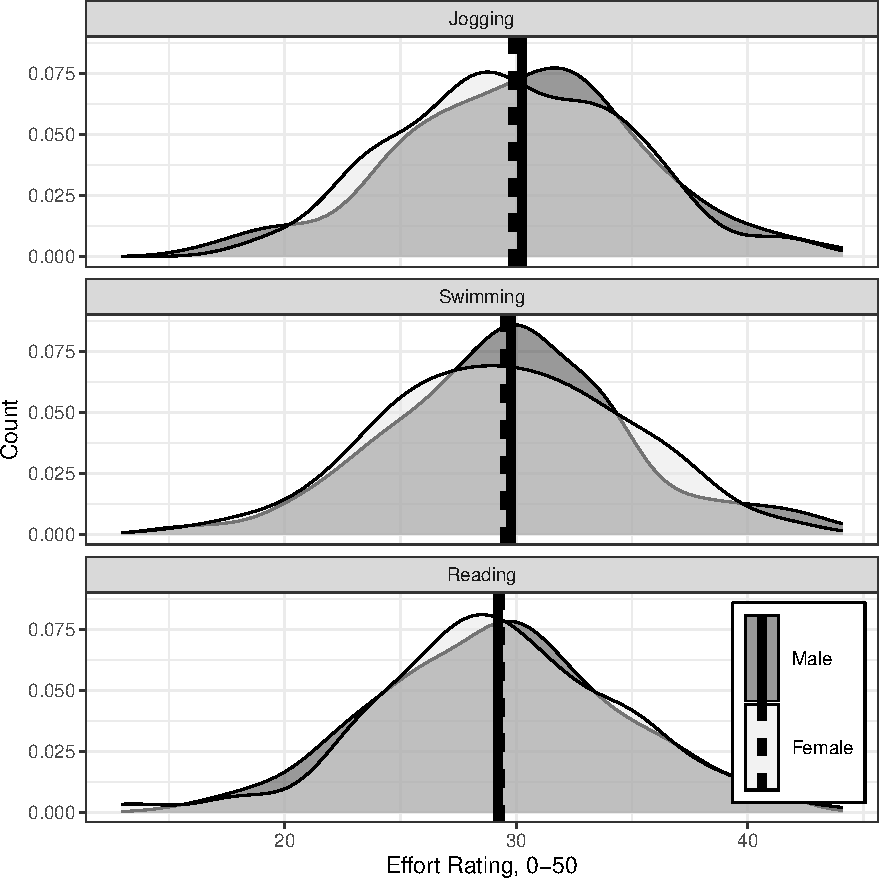
\includegraphics{Appendix_ex_weightloss_files/figure-latex/unnamed-chunk-57-1} \hfill{}

\caption{Distribution of Effort Rating, By Program and Gender - Option A}\label{fig:unnamed-chunk-57}
\end{figure}

\clearpage

\begin{Shaded}
\begin{Highlighting}[]
\NormalTok{df\_use }\SpecialCharTok{\%\textgreater{}\%} 
  \FunctionTok{ggplot}\NormalTok{(}\FunctionTok{aes}\NormalTok{(}\AttributeTok{x =}\NormalTok{ prog,}
             \AttributeTok{y =}\NormalTok{ effort,}
             \AttributeTok{fill =}\NormalTok{ gender,}
             \AttributeTok{shape =}\NormalTok{ gender,}
             \AttributeTok{group =} \FunctionTok{interaction}\NormalTok{(prog,gender))) }\SpecialCharTok{+} 
  \FunctionTok{geom\_violin}\NormalTok{(}\AttributeTok{alpha =}\NormalTok{ .}\DecValTok{5}\NormalTok{) }\SpecialCharTok{+}
  \FunctionTok{geom\_boxplot}\NormalTok{(}\AttributeTok{fill =} \StringTok{"white"}\NormalTok{,}
               \AttributeTok{width =}\NormalTok{ .}\DecValTok{25}\NormalTok{,}
               \AttributeTok{position =} \FunctionTok{position\_dodge}\NormalTok{(}\AttributeTok{width =}\NormalTok{ .}\DecValTok{9}\NormalTok{)) }\SpecialCharTok{+}
  \FunctionTok{stat\_summary}\NormalTok{(}\AttributeTok{fun =}\NormalTok{ mean,}
               \AttributeTok{geom =} \StringTok{"point"}\NormalTok{,}
               \AttributeTok{size =} \DecValTok{5}\NormalTok{,}
               \AttributeTok{position =} \FunctionTok{position\_dodge}\NormalTok{(}\AttributeTok{width =}\NormalTok{ .}\DecValTok{9}\NormalTok{)) }\SpecialCharTok{+}
  \FunctionTok{labs}\NormalTok{(}\AttributeTok{x =} \StringTok{"Program, randomized"}\NormalTok{,}
       \AttributeTok{y =} \StringTok{"Effort Rating, 0{-}50"}\NormalTok{,}
       \AttributeTok{fill =} \ConstantTok{NULL}\NormalTok{,}
       \AttributeTok{color =} \ConstantTok{NULL}\NormalTok{,}
       \AttributeTok{shape =} \ConstantTok{NULL}\NormalTok{)  }\SpecialCharTok{+}
  \FunctionTok{scale\_fill\_manual}\NormalTok{(}\AttributeTok{values =} \FunctionTok{c}\NormalTok{(}\StringTok{"gray20"}\NormalTok{, }\StringTok{"gray90"}\NormalTok{)) }\SpecialCharTok{+}
  \FunctionTok{scale\_shape\_manual}\NormalTok{(}\AttributeTok{values =} \FunctionTok{c}\NormalTok{(}\DecValTok{18}\NormalTok{, }\DecValTok{19}\NormalTok{)) }\SpecialCharTok{+}
  \FunctionTok{theme}\NormalTok{(}\AttributeTok{legend.key.height =} \FunctionTok{unit}\NormalTok{(}\DecValTok{2}\NormalTok{, }\StringTok{"cm"}\NormalTok{))}
\end{Highlighting}
\end{Shaded}

\begin{figure}[hb]

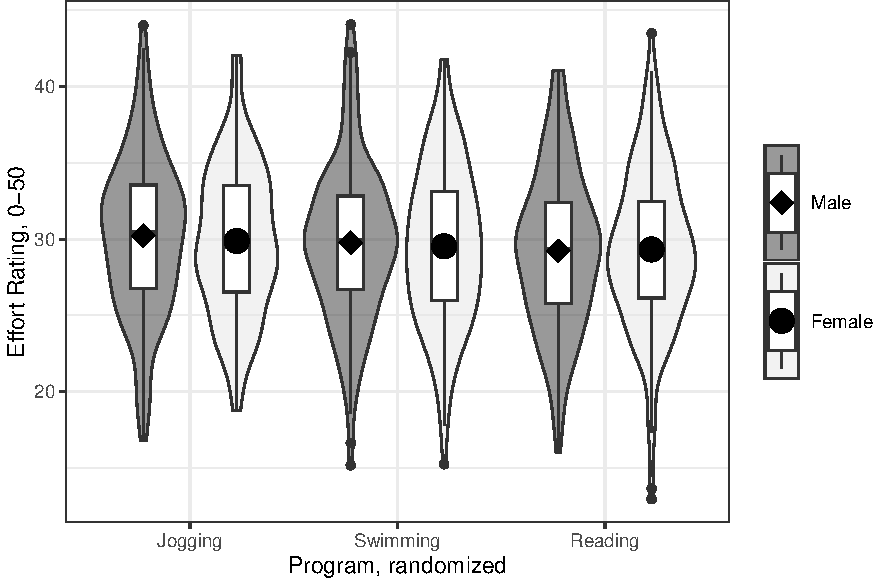
\includegraphics{Appendix_ex_weightloss_files/figure-latex/unnamed-chunk-59-1} \hfill{}

\caption{Distribution of Effort Rating, By Program and Gender - Option B}\label{fig:unnamed-chunk-59}
\end{figure}

\clearpage

\begin{Shaded}
\begin{Highlighting}[]
\NormalTok{df\_use }\SpecialCharTok{\%\textgreater{}\%} 
  \FunctionTok{ggplot}\NormalTok{(}\FunctionTok{aes}\NormalTok{(}\AttributeTok{x =}\NormalTok{ gender,}
             \AttributeTok{y =}\NormalTok{ effort,}
             \AttributeTok{shape =}\NormalTok{ gender,}
             \AttributeTok{group =}\NormalTok{ gender)) }\SpecialCharTok{+} 
  \FunctionTok{geom\_violin}\NormalTok{(}\AttributeTok{fill =} \StringTok{"gray"}\NormalTok{,}
              \AttributeTok{alpha =}\NormalTok{ .}\DecValTok{5}\NormalTok{) }\SpecialCharTok{+}
  \FunctionTok{geom\_boxplot}\NormalTok{(}\AttributeTok{fill =} \StringTok{"white"}\NormalTok{,}
               \AttributeTok{width =}\NormalTok{ .}\DecValTok{25}\NormalTok{,}
               \AttributeTok{position =} \FunctionTok{position\_dodge}\NormalTok{(}\AttributeTok{width =}\NormalTok{ .}\DecValTok{9}\NormalTok{)) }\SpecialCharTok{+}
  \FunctionTok{stat\_summary}\NormalTok{(}\AttributeTok{fun =}\NormalTok{ mean,}
               \AttributeTok{geom =} \StringTok{"point"}\NormalTok{,}
               \AttributeTok{size =} \DecValTok{5}\NormalTok{,}
               \AttributeTok{position =} \FunctionTok{position\_dodge}\NormalTok{(}\AttributeTok{width =}\NormalTok{ .}\DecValTok{9}\NormalTok{)) }\SpecialCharTok{+}
  \FunctionTok{stat\_summary}\NormalTok{(}\FunctionTok{aes}\NormalTok{(}\AttributeTok{group =} \DecValTok{1}\NormalTok{),}
               \AttributeTok{fun =} \StringTok{"mean"}\NormalTok{,}
               \AttributeTok{geom =} \StringTok{"line"}\NormalTok{) }\SpecialCharTok{+}
  \FunctionTok{labs}\NormalTok{(}\AttributeTok{x =} \ConstantTok{NULL}\NormalTok{,}
       \AttributeTok{y =} \StringTok{"Effort Rating, 0{-}50"}\NormalTok{,}
       \AttributeTok{shape =} \ConstantTok{NULL}\NormalTok{)  }\SpecialCharTok{+}
  \FunctionTok{scale\_shape\_manual}\NormalTok{(}\AttributeTok{values =} \FunctionTok{c}\NormalTok{(}\DecValTok{18}\NormalTok{, }\DecValTok{19}\NormalTok{)) }\SpecialCharTok{+}
  \FunctionTok{theme}\NormalTok{(}\AttributeTok{legend.position =} \StringTok{"none"}\NormalTok{) }\SpecialCharTok{+}
  \FunctionTok{facet\_grid}\NormalTok{(}\SpecialCharTok{\textasciitilde{}}\NormalTok{ prog)}
\end{Highlighting}
\end{Shaded}

\begin{figure}[hb]

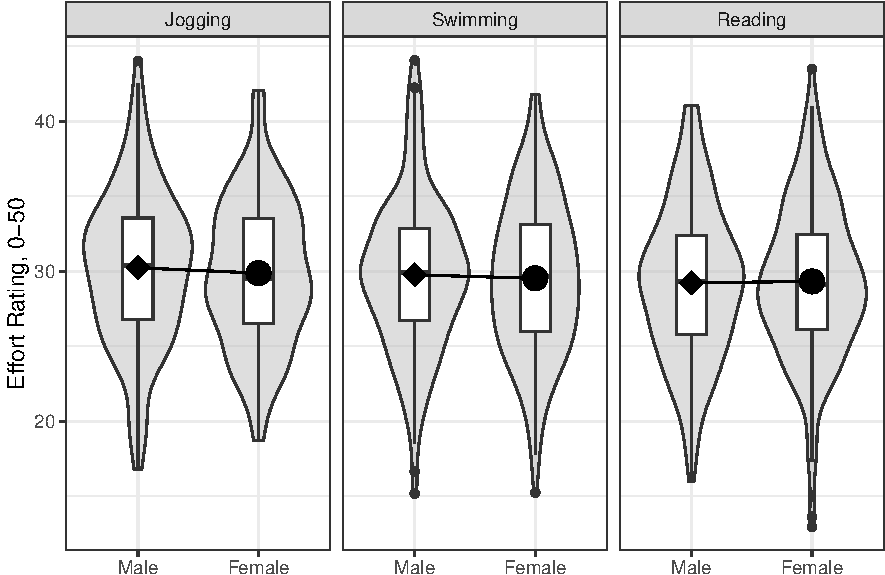
\includegraphics{Appendix_ex_weightloss_files/figure-latex/unnamed-chunk-61-1} \hfill{}

\caption{Distribution of Effort Rating, By Program and Gender - Option C}\label{fig:unnamed-chunk-61}
\end{figure}

\clearpage

\hypertarget{bivariable}{%
\subsection{Bivariable}\label{bivariable}}

\hypertarget{weight-loss-by-program-time}{%
\subsubsection{Weight Loss by Program
Time}\label{weight-loss-by-program-time}}

\begin{Shaded}
\begin{Highlighting}[]
\NormalTok{df\_use }\SpecialCharTok{\%\textgreater{}\%} 
  \FunctionTok{ggplot}\NormalTok{(}\FunctionTok{aes}\NormalTok{(}\AttributeTok{x =}\NormalTok{ hours,}
             \AttributeTok{y =}\NormalTok{ loss)) }\SpecialCharTok{+}
  \FunctionTok{geom\_hline}\NormalTok{(}\AttributeTok{yintercept =} \DecValTok{0}\NormalTok{, }\AttributeTok{color =} \StringTok{"black"}\NormalTok{) }\SpecialCharTok{+}
  \FunctionTok{geom\_point}\NormalTok{(}\AttributeTok{alpha =}\NormalTok{ .}\DecValTok{25}\NormalTok{) }\SpecialCharTok{+}
  \FunctionTok{theme\_bw}\NormalTok{() }\SpecialCharTok{+}
  \FunctionTok{facet\_grid}\NormalTok{(gender }\SpecialCharTok{\textasciitilde{}}\NormalTok{ prog) }\SpecialCharTok{+}
  \FunctionTok{geom\_smooth}\NormalTok{(}\AttributeTok{method =} \StringTok{"lm"}\NormalTok{,}
              \AttributeTok{formula =}\NormalTok{ y }\SpecialCharTok{\textasciitilde{}}\NormalTok{ x,}
              \AttributeTok{se =} \ConstantTok{FALSE}\NormalTok{,}
              \AttributeTok{linetype =} \StringTok{"longdash"}\NormalTok{) }\SpecialCharTok{+}
\NormalTok{  ggpubr}\SpecialCharTok{::}\FunctionTok{stat\_cor}\NormalTok{(}\FunctionTok{aes}\NormalTok{(}\AttributeTok{label =}\NormalTok{ ..r.label..),}
                   \AttributeTok{cor.coef.name =} \StringTok{"r"}\NormalTok{,}
                   \AttributeTok{digits =} \DecValTok{3}\NormalTok{)}
\end{Highlighting}
\end{Shaded}

\begin{figure}[hb]

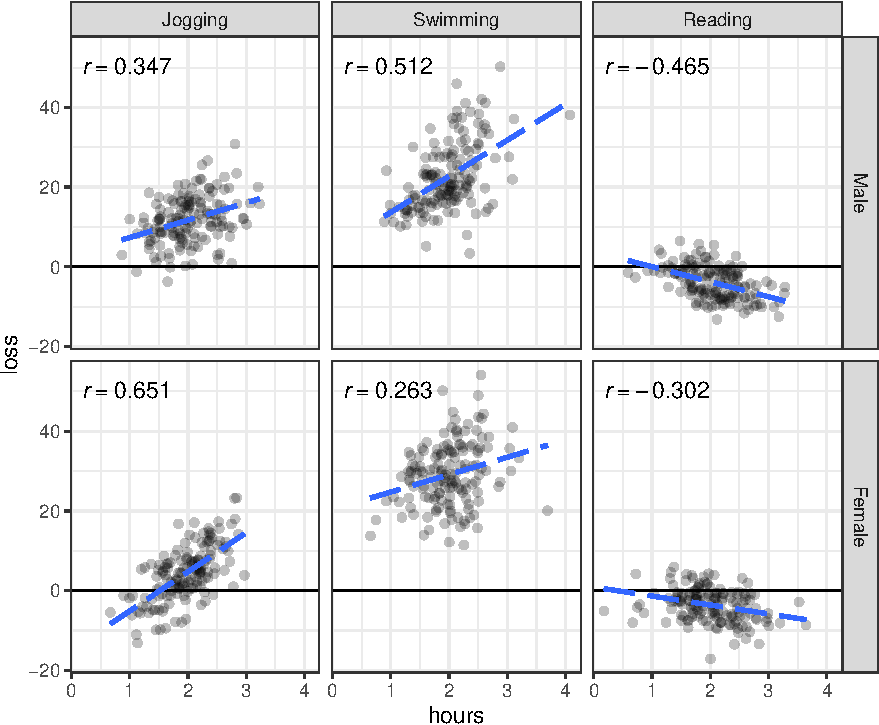
\includegraphics{Appendix_ex_weightloss_files/figure-latex/unnamed-chunk-63-1} \hfill{}

\caption{Association Between Weight Loss by Program Time, by Gender and Program}\label{fig:unnamed-chunk-63}
\end{figure}

\clearpage

\hypertarget{weight-loss-by-effort-rating}{%
\subsubsection{Weight Loss by Effort
Rating}\label{weight-loss-by-effort-rating}}

\begin{Shaded}
\begin{Highlighting}[]
\NormalTok{df\_use }\SpecialCharTok{\%\textgreater{}\%} 
  \FunctionTok{ggplot}\NormalTok{(}\FunctionTok{aes}\NormalTok{(}\AttributeTok{x =}\NormalTok{ effort,}
             \AttributeTok{y =}\NormalTok{ loss)) }\SpecialCharTok{+}
  \FunctionTok{geom\_hline}\NormalTok{(}\AttributeTok{yintercept =} \DecValTok{0}\NormalTok{, }\AttributeTok{color =} \StringTok{"black"}\NormalTok{) }\SpecialCharTok{+}
  \FunctionTok{geom\_point}\NormalTok{(}\AttributeTok{alpha =}\NormalTok{ .}\DecValTok{25}\NormalTok{) }\SpecialCharTok{+}
  \FunctionTok{theme\_bw}\NormalTok{() }\SpecialCharTok{+}
  \FunctionTok{facet\_grid}\NormalTok{(gender }\SpecialCharTok{\textasciitilde{}}\NormalTok{ prog) }\SpecialCharTok{+}
  \FunctionTok{geom\_smooth}\NormalTok{(}\AttributeTok{method =} \StringTok{"lm"}\NormalTok{,}
              \AttributeTok{formula =}\NormalTok{ y }\SpecialCharTok{\textasciitilde{}}\NormalTok{ x,}
              \AttributeTok{se =} \ConstantTok{FALSE}\NormalTok{,}
              \AttributeTok{linetype =} \StringTok{"longdash"}\NormalTok{) }\SpecialCharTok{+}
\NormalTok{  ggpubr}\SpecialCharTok{::}\FunctionTok{stat\_cor}\NormalTok{(}\FunctionTok{aes}\NormalTok{(}\AttributeTok{label =}\NormalTok{ ..r.label..),}
                   \AttributeTok{cor.coef.name =} \StringTok{"r"}\NormalTok{,}
                   \AttributeTok{digits =} \DecValTok{3}\NormalTok{,}
                   \AttributeTok{r.accuracy =}\NormalTok{ .}\DecValTok{001}\NormalTok{)}
\end{Highlighting}
\end{Shaded}

\begin{figure}[hb]

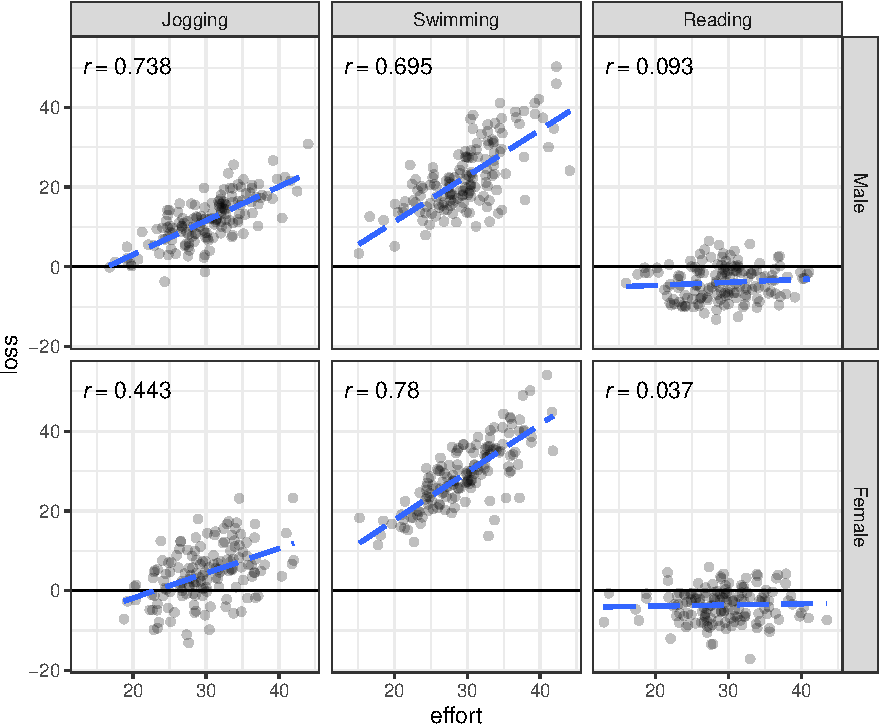
\includegraphics{Appendix_ex_weightloss_files/figure-latex/unnamed-chunk-65-1} \hfill{}

\caption{Association Between Weight Loss by Effort Rating, by Gender and Program}\label{fig:unnamed-chunk-65}
\end{figure}

\clearpage

\hypertarget{effort-rating-by-program-time}{%
\subsubsection{Effort Rating by Program
Time}\label{effort-rating-by-program-time}}

\begin{Shaded}
\begin{Highlighting}[]
\NormalTok{df\_use }\SpecialCharTok{\%\textgreater{}\%} 
  \FunctionTok{ggplot}\NormalTok{(}\FunctionTok{aes}\NormalTok{(}\AttributeTok{x =}\NormalTok{ hours,}
             \AttributeTok{y =}\NormalTok{ effort)) }\SpecialCharTok{+}
  \FunctionTok{geom\_point}\NormalTok{(}\AttributeTok{alpha =}\NormalTok{ .}\DecValTok{25}\NormalTok{) }\SpecialCharTok{+}
  \FunctionTok{theme\_bw}\NormalTok{() }\SpecialCharTok{+}
  \FunctionTok{facet\_grid}\NormalTok{(gender }\SpecialCharTok{\textasciitilde{}}\NormalTok{ prog) }\SpecialCharTok{+}
  \FunctionTok{geom\_smooth}\NormalTok{(}\AttributeTok{method =} \StringTok{"lm"}\NormalTok{,}
              \AttributeTok{formula =}\NormalTok{ y }\SpecialCharTok{\textasciitilde{}}\NormalTok{ x,}
              \AttributeTok{se =} \ConstantTok{FALSE}\NormalTok{,}
              \AttributeTok{linetype =} \StringTok{"longdash"}\NormalTok{) }\SpecialCharTok{+}
\NormalTok{  ggpubr}\SpecialCharTok{::}\FunctionTok{stat\_cor}\NormalTok{(}\FunctionTok{aes}\NormalTok{(}\AttributeTok{label =}\NormalTok{ ..r.label..),}
                   \AttributeTok{cor.coef.name =} \StringTok{"r"}\NormalTok{,}
                   \AttributeTok{digits =} \DecValTok{3}\NormalTok{)}
\end{Highlighting}
\end{Shaded}

\begin{figure}[hb]

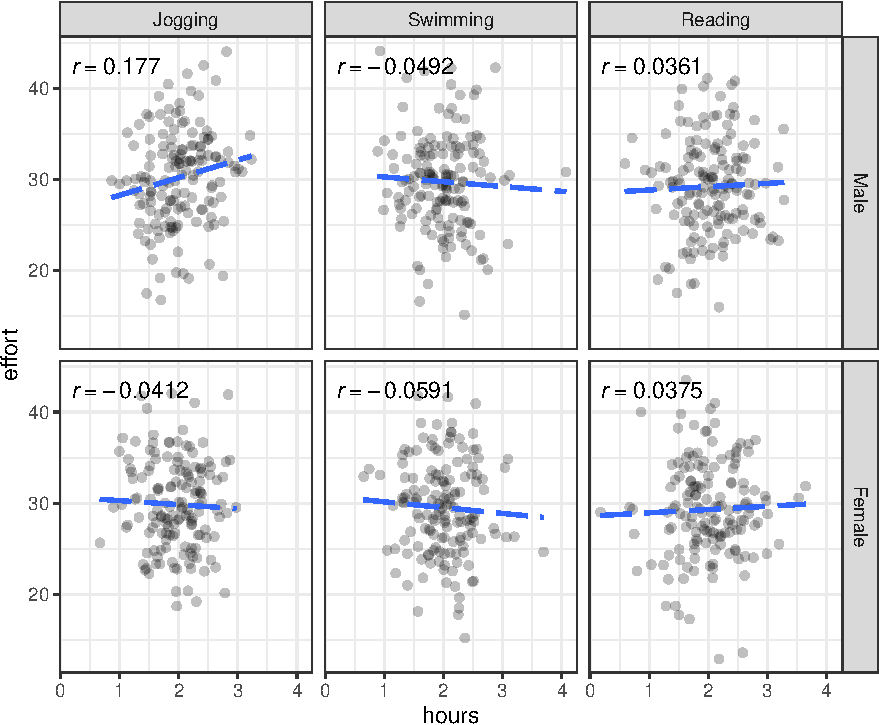
\includegraphics{Appendix_ex_weightloss_files/figure-latex/unnamed-chunk-67-1} \hfill{}

\caption{Association Between Effort Rating by Program Time, by Gender and Program}\label{fig:unnamed-chunk-67}
\end{figure}

\clearpage

\hypertarget{regression-analysis}{%
\section{REGRESSION ANALYSIS}\label{regression-analysis}}

Multip

\hypertarget{model-fitting}{%
\subsection{Model Fitting}\label{model-fitting}}

\hypertarget{fit-nested-models}{%
\subsubsection{Fit Nested Models}\label{fit-nested-models}}

\begin{Shaded}
\begin{Highlighting}[]
\NormalTok{fit\_1 }\OtherTok{\textless{}{-}} \FunctionTok{lm}\NormalTok{(loss }\SpecialCharTok{\textasciitilde{}}\NormalTok{ prog }\SpecialCharTok{+}\NormalTok{ hours }\SpecialCharTok{+}\NormalTok{ gender }\SpecialCharTok{+}\NormalTok{ effort,}
            \AttributeTok{data =}\NormalTok{ df\_use)}

\NormalTok{fit\_2 }\OtherTok{\textless{}{-}} \FunctionTok{lm}\NormalTok{(loss }\SpecialCharTok{\textasciitilde{}}\NormalTok{ prog}\SpecialCharTok{*}\NormalTok{hours}\SpecialCharTok{*}\NormalTok{gender }\SpecialCharTok{+} 
\NormalTok{              prog}\SpecialCharTok{*}\NormalTok{hours}\SpecialCharTok{*}\NormalTok{effort,}
            \AttributeTok{data =}\NormalTok{ df\_use)}

\NormalTok{fit\_3 }\OtherTok{\textless{}{-}} \FunctionTok{lm}\NormalTok{(loss }\SpecialCharTok{\textasciitilde{}}\NormalTok{ prog}\SpecialCharTok{*}\NormalTok{hours}\SpecialCharTok{*}\NormalTok{gender }\SpecialCharTok{+} 
\NormalTok{              prog}\SpecialCharTok{*}\NormalTok{gender}\SpecialCharTok{*}\NormalTok{effort }\SpecialCharTok{+} 
\NormalTok{              prog}\SpecialCharTok{*}\NormalTok{hours}\SpecialCharTok{*}\NormalTok{effort,}
            \AttributeTok{data =}\NormalTok{ df\_use)}
\NormalTok{fit\_4 }\OtherTok{\textless{}{-}} \FunctionTok{lm}\NormalTok{(loss }\SpecialCharTok{\textasciitilde{}}\NormalTok{ prog}\SpecialCharTok{*}\NormalTok{hours}\SpecialCharTok{*}\NormalTok{gender}\SpecialCharTok{*}\NormalTok{effort,}
            \AttributeTok{data =}\NormalTok{ df\_use)}
\end{Highlighting}
\end{Shaded}

\clearpage

\hypertarget{parameter-estimate-table}{%
\subsubsection{Parameter Estimate
Table}\label{parameter-estimate-table}}

\begin{Shaded}
\begin{Highlighting}[]
\NormalTok{texreg}\SpecialCharTok{::}\FunctionTok{knitreg}\NormalTok{(}\FunctionTok{list}\NormalTok{(fit\_1, fit\_2, fit\_3, fit\_4),}
                \AttributeTok{custom.model.names =} \FunctionTok{c}\NormalTok{(}\StringTok{"fit 1"}\NormalTok{, }\StringTok{"fit 2"}\NormalTok{, }\StringTok{"fit 3"}\NormalTok{, }\StringTok{"fit 4"}\NormalTok{),}
                \AttributeTok{caption =} \StringTok{"Parameter Estimates of Nested Regression Models for Weight Loss"}\NormalTok{)}
\end{Highlighting}
\end{Shaded}

\begin{table}
\begin{center}
\begin{tabular}{l c c c c}
\hline
 & fit 1 & fit 2 & fit 3 & fit 4 \\
\hline
(Intercept)                            & $-17.80^{***}$ & $2.18$         & $-0.03$        & $7.42$        \\
                                       & $(1.49)$       & $(6.39)$       & $(6.58)$       & $(9.15)$      \\
progSwimming                           & $18.05^{***}$  & $8.30$         & $10.80$        & $-1.74$       \\
                                       & $(0.50)$       & $(8.76)$       & $(8.99)$       & $(12.05)$     \\
progReading                            & $-11.45^{***}$ & $6.08$         & $7.46$         & $2.91$        \\
                                       & $(0.50)$       & $(8.38)$       & $(8.68)$       & $(12.11)$     \\
hours                                  & $3.14^{***}$   & $-6.46^{*}$    & $-6.27^{*}$    & $-9.98^{*}$   \\
                                       & $(0.41)$       & $(3.17)$       & $(3.17)$       & $(4.48)$      \\
genderFemale                           & $0.01$         & $-20.95^{***}$ & $-17.34^{***}$ & $-31.80^{*}$  \\
                                       & $(0.41)$       & $(1.97)$       & $(3.24)$       & $(12.75)$     \\
effort                                 & $0.65^{***}$   & $0.12$         & $0.20$         & $-0.04$       \\
                                       & $(0.04)$       & $(0.21)$       & $(0.22)$       & $(0.30)$      \\
progSwimming:hours                     &                & $-5.15$        & $-5.34$        & $0.89$        \\
                                       &                & $(4.28)$       & $(4.28)$       & $(5.84)$      \\
progReading:hours                      &                & $-0.52$        & $-0.62$        & $1.63$        \\
                                       &                & $(4.15)$       & $(4.16)$       & $(5.92)$      \\
progSwimming:genderFemale              &                & $35.59^{***}$  & $31.35^{***}$  & $57.63^{***}$ \\
                                       &                & $(2.73)$       & $(4.60)$       & $(17.38)$     \\
progReading:genderFemale               &                & $18.00^{***}$  & $15.62^{***}$  & $24.74$       \\
                                       &                & $(2.65)$       & $(4.44)$       & $(16.66)$     \\
hours:genderFemale                     &                & $7.18^{***}$   & $7.27^{***}$   & $14.55^{*}$   \\
                                       &                & $(0.97)$       & $(0.97)$       & $(6.28)$      \\
progSwimming:effort                    &                & $-0.33$        & $-0.42$        & $-0.00$       \\
                                       &                & $(0.28)$       & $(0.29)$       & $(0.39)$      \\
progReading:effort                     &                & $-0.27$        & $-0.33$        & $-0.18$       \\
                                       &                & $(0.28)$       & $(0.29)$       & $(0.40)$      \\
hours:effort                           &                & $0.31^{**}$    & $0.30^{**}$    & $0.42^{**}$   \\
                                       &                & $(0.10)$       & $(0.10)$       & $(0.15)$      \\
progSwimming:hours:genderFemale        &                & $-11.15^{***}$ & $-11.23^{***}$ & $-24.32^{**}$ \\
                                       &                & $(1.34)$       & $(1.34)$       & $(8.45)$      \\
progReading:hours:genderFemale         &                & $-5.63^{***}$  & $-5.70^{***}$  & $-10.25$      \\
                                       &                & $(1.28)$       & $(1.29)$       & $(8.22)$      \\
progSwimming:hours:effort              &                & $0.39^{**}$    & $0.40^{**}$    & $0.20$        \\
                                       &                & $(0.14)$       & $(0.14)$       & $(0.19)$      \\
progReading:hours:effort               &                & $-0.20$        & $-0.19$        & $-0.26$       \\
                                       &                & $(0.14)$       & $(0.14)$       & $(0.20)$      \\
genderFemale:effort                    &                &                & $-0.13$        & $0.35$        \\
                                       &                &                & $(0.09)$       & $(0.42)$      \\
progSwimming:genderFemale:effort       &                &                & $0.15$         & $-0.72$       \\
                                       &                &                & $(0.12)$       & $(0.57)$      \\
progReading:genderFemale:effort        &                &                & $0.08$         & $-0.21$       \\
                                       &                &                & $(0.12)$       & $(0.55)$      \\
hours:genderFemale:effort              &                &                &                & $-0.24$       \\
                                       &                &                &                & $(0.20)$      \\
progSwimming:hours:genderFemale:effort &                &                &                & $0.43$        \\
                                       &                &                &                & $(0.28)$      \\
progReading:hours:genderFemale:effort  &                &                &                & $0.14$        \\
                                       &                &                &                & $(0.27)$      \\
\hline
R$^2$                                  & $0.82$         & $0.93$         & $0.93$         & $0.93$        \\
Adj. R$^2$                             & $0.81$         & $0.92$         & $0.92$         & $0.92$        \\
Num. obs.                              & $900$          & $900$          & $900$          & $900$         \\
\hline
\multicolumn{5}{l}{\scriptsize{$^{***}p<0.001$; $^{**}p<0.01$; $^{*}p<0.05$}}
\end{tabular}
\caption{Parameter Estimates of Nested Regression Models for Weight Loss}
\label{table:coefficients}
\end{center}
\end{table}

\clearpage

\hypertarget{compare-model-fit}{%
\subsubsection{Compare Model Fit}\label{compare-model-fit}}

\begin{Shaded}
\begin{Highlighting}[]
\NormalTok{tab\_lm\_fits }\OtherTok{\textless{}{-}}\NormalTok{ performance}\SpecialCharTok{::}\FunctionTok{compare\_performance}\NormalTok{(fit\_1, fit\_2, fit\_3, fit\_4) }\SpecialCharTok{\%\textgreater{}\%} 
  \FunctionTok{data.frame}\NormalTok{() }\SpecialCharTok{\%\textgreater{}\%} 
\NormalTok{  dplyr}\SpecialCharTok{::}\FunctionTok{select}\NormalTok{(Name, AIC, BIC, R2, R2\_adjusted, RMSE, Sigma) }\SpecialCharTok{\%\textgreater{}\%} 
\NormalTok{  flextable}\SpecialCharTok{::}\FunctionTok{flextable}\NormalTok{() }\SpecialCharTok{\%\textgreater{}\%} 
\NormalTok{  flextable}\SpecialCharTok{::}\FunctionTok{set\_caption}\NormalTok{(}\StringTok{"Comparison of Model Fit for Nested Regression Models for Weight Loss"}\NormalTok{)}

\NormalTok{tab\_lm\_fits}
\end{Highlighting}
\end{Shaded}

\global\setlength{\Oldarrayrulewidth}{\arrayrulewidth}

\global\setlength{\Oldtabcolsep}{\tabcolsep}

\setlength{\tabcolsep}{2pt}

\renewcommand*{\arraystretch}{1.5}



\providecommand{\ascline}[3]{\noalign{\global\arrayrulewidth #1}\arrayrulecolor[HTML]{#2}\cline{#3}}

\begin{longtable}[l]{|p{0.75in}|p{0.75in}|p{0.75in}|p{0.75in}|p{0.75in}|p{0.75in}|p{0.75in}}

\caption{Comparison\ of\ Model\ Fit\ for\ Nested\ Regression\ Models\ for\ Weight\ Loss}\\

\ascline{0.75pt}{000000}{1-7}

\multicolumn{1}{>{\centering}m{\dimexpr 0.75in+0\tabcolsep}}{\textcolor[HTML]{000000}{\fontsize{10}{20}\selectfont{\global\setmainfont{Times New Roman}{Name}}}} & \multicolumn{1}{>{\centering}m{\dimexpr 0.75in+0\tabcolsep}}{\textcolor[HTML]{000000}{\fontsize{10}{20}\selectfont{\global\setmainfont{Times New Roman}{AIC}}}} & \multicolumn{1}{>{\centering}m{\dimexpr 0.75in+0\tabcolsep}}{\textcolor[HTML]{000000}{\fontsize{10}{20}\selectfont{\global\setmainfont{Times New Roman}{BIC}}}} & \multicolumn{1}{>{\centering}m{\dimexpr 0.75in+0\tabcolsep}}{\textcolor[HTML]{000000}{\fontsize{10}{20}\selectfont{\global\setmainfont{Times New Roman}{R2}}}} & \multicolumn{1}{>{\centering}m{\dimexpr 0.75in+0\tabcolsep}}{\textcolor[HTML]{000000}{\fontsize{10}{20}\selectfont{\global\setmainfont{Times New Roman}{R2\_adjusted}}}} & \multicolumn{1}{>{\centering}m{\dimexpr 0.75in+0\tabcolsep}}{\textcolor[HTML]{000000}{\fontsize{10}{20}\selectfont{\global\setmainfont{Times New Roman}{RMSE}}}} & \multicolumn{1}{>{\centering}m{\dimexpr 0.75in+0\tabcolsep}}{\textcolor[HTML]{000000}{\fontsize{10}{20}\selectfont{\global\setmainfont{Times New Roman}{Sigma}}}} \\

\ascline{0.75pt}{000000}{1-7}\endfirsthead \caption[]{Comparison\ of\ Model\ Fit\ for\ Nested\ Regression\ Models\ for\ Weight\ Loss}\\

\ascline{0.75pt}{000000}{1-7}

\multicolumn{1}{>{\centering}m{\dimexpr 0.75in+0\tabcolsep}}{\textcolor[HTML]{000000}{\fontsize{10}{20}\selectfont{\global\setmainfont{Times New Roman}{Name}}}} & \multicolumn{1}{>{\centering}m{\dimexpr 0.75in+0\tabcolsep}}{\textcolor[HTML]{000000}{\fontsize{10}{20}\selectfont{\global\setmainfont{Times New Roman}{AIC}}}} & \multicolumn{1}{>{\centering}m{\dimexpr 0.75in+0\tabcolsep}}{\textcolor[HTML]{000000}{\fontsize{10}{20}\selectfont{\global\setmainfont{Times New Roman}{BIC}}}} & \multicolumn{1}{>{\centering}m{\dimexpr 0.75in+0\tabcolsep}}{\textcolor[HTML]{000000}{\fontsize{10}{20}\selectfont{\global\setmainfont{Times New Roman}{R2}}}} & \multicolumn{1}{>{\centering}m{\dimexpr 0.75in+0\tabcolsep}}{\textcolor[HTML]{000000}{\fontsize{10}{20}\selectfont{\global\setmainfont{Times New Roman}{R2\_adjusted}}}} & \multicolumn{1}{>{\centering}m{\dimexpr 0.75in+0\tabcolsep}}{\textcolor[HTML]{000000}{\fontsize{10}{20}\selectfont{\global\setmainfont{Times New Roman}{RMSE}}}} & \multicolumn{1}{>{\centering}m{\dimexpr 0.75in+0\tabcolsep}}{\textcolor[HTML]{000000}{\fontsize{10}{20}\selectfont{\global\setmainfont{Times New Roman}{Sigma}}}} \\

\ascline{0.75pt}{000000}{1-7}\endhead



\multicolumn{1}{>{\centering}m{\dimexpr 0.75in+0\tabcolsep}}{\textcolor[HTML]{000000}{\fontsize{10}{20}\selectfont{\global\setmainfont{Times New Roman}{fit\_1}}}} & \multicolumn{1}{>{\centering}m{\dimexpr 0.75in+0\tabcolsep}}{\textcolor[HTML]{000000}{\fontsize{10}{20}\selectfont{\global\setmainfont{Times New Roman}{5,811.56}}}} & \multicolumn{1}{>{\centering}m{\dimexpr 0.75in+0\tabcolsep}}{\textcolor[HTML]{000000}{\fontsize{10}{20}\selectfont{\global\setmainfont{Times New Roman}{5,845.18}}}} & \multicolumn{1}{>{\centering}m{\dimexpr 0.75in+0\tabcolsep}}{\textcolor[HTML]{000000}{\fontsize{10}{20}\selectfont{\global\setmainfont{Times New Roman}{0.82}}}} & \multicolumn{1}{>{\centering}m{\dimexpr 0.75in+0\tabcolsep}}{\textcolor[HTML]{000000}{\fontsize{10}{20}\selectfont{\global\setmainfont{Times New Roman}{0.81}}}} & \multicolumn{1}{>{\centering}m{\dimexpr 0.75in+0\tabcolsep}}{\textcolor[HTML]{000000}{\fontsize{10}{20}\selectfont{\global\setmainfont{Times New Roman}{6.06}}}} & \multicolumn{1}{>{\centering}m{\dimexpr 0.75in+0\tabcolsep}}{\textcolor[HTML]{000000}{\fontsize{10}{20}\selectfont{\global\setmainfont{Times New Roman}{6.08}}}} \\





\multicolumn{1}{>{\centering}m{\dimexpr 0.75in+0\tabcolsep}}{\textcolor[HTML]{000000}{\fontsize{10}{20}\selectfont{\global\setmainfont{Times New Roman}{fit\_2}}}} & \multicolumn{1}{>{\centering}m{\dimexpr 0.75in+0\tabcolsep}}{\textcolor[HTML]{000000}{\fontsize{10}{20}\selectfont{\global\setmainfont{Times New Roman}{5,006.15}}}} & \multicolumn{1}{>{\centering}m{\dimexpr 0.75in+0\tabcolsep}}{\textcolor[HTML]{000000}{\fontsize{10}{20}\selectfont{\global\setmainfont{Times New Roman}{5,097.40}}}} & \multicolumn{1}{>{\centering}m{\dimexpr 0.75in+0\tabcolsep}}{\textcolor[HTML]{000000}{\fontsize{10}{20}\selectfont{\global\setmainfont{Times New Roman}{0.93}}}} & \multicolumn{1}{>{\centering}m{\dimexpr 0.75in+0\tabcolsep}}{\textcolor[HTML]{000000}{\fontsize{10}{20}\selectfont{\global\setmainfont{Times New Roman}{0.92}}}} & \multicolumn{1}{>{\centering}m{\dimexpr 0.75in+0\tabcolsep}}{\textcolor[HTML]{000000}{\fontsize{10}{20}\selectfont{\global\setmainfont{Times New Roman}{3.82}}}} & \multicolumn{1}{>{\centering}m{\dimexpr 0.75in+0\tabcolsep}}{\textcolor[HTML]{000000}{\fontsize{10}{20}\selectfont{\global\setmainfont{Times New Roman}{3.86}}}} \\





\multicolumn{1}{>{\centering}m{\dimexpr 0.75in+0\tabcolsep}}{\textcolor[HTML]{000000}{\fontsize{10}{20}\selectfont{\global\setmainfont{Times New Roman}{fit\_3}}}} & \multicolumn{1}{>{\centering}m{\dimexpr 0.75in+0\tabcolsep}}{\textcolor[HTML]{000000}{\fontsize{10}{20}\selectfont{\global\setmainfont{Times New Roman}{5,009.82}}}} & \multicolumn{1}{>{\centering}m{\dimexpr 0.75in+0\tabcolsep}}{\textcolor[HTML]{000000}{\fontsize{10}{20}\selectfont{\global\setmainfont{Times New Roman}{5,115.47}}}} & \multicolumn{1}{>{\centering}m{\dimexpr 0.75in+0\tabcolsep}}{\textcolor[HTML]{000000}{\fontsize{10}{20}\selectfont{\global\setmainfont{Times New Roman}{0.93}}}} & \multicolumn{1}{>{\centering}m{\dimexpr 0.75in+0\tabcolsep}}{\textcolor[HTML]{000000}{\fontsize{10}{20}\selectfont{\global\setmainfont{Times New Roman}{0.92}}}} & \multicolumn{1}{>{\centering}m{\dimexpr 0.75in+0\tabcolsep}}{\textcolor[HTML]{000000}{\fontsize{10}{20}\selectfont{\global\setmainfont{Times New Roman}{3.82}}}} & \multicolumn{1}{>{\centering}m{\dimexpr 0.75in+0\tabcolsep}}{\textcolor[HTML]{000000}{\fontsize{10}{20}\selectfont{\global\setmainfont{Times New Roman}{3.86}}}} \\





\multicolumn{1}{>{\centering}m{\dimexpr 0.75in+0\tabcolsep}}{\textcolor[HTML]{000000}{\fontsize{10}{20}\selectfont{\global\setmainfont{Times New Roman}{fit\_4}}}} & \multicolumn{1}{>{\centering}m{\dimexpr 0.75in+0\tabcolsep}}{\textcolor[HTML]{000000}{\fontsize{10}{20}\selectfont{\global\setmainfont{Times New Roman}{5,013.01}}}} & \multicolumn{1}{>{\centering}m{\dimexpr 0.75in+0\tabcolsep}}{\textcolor[HTML]{000000}{\fontsize{10}{20}\selectfont{\global\setmainfont{Times New Roman}{5,133.07}}}} & \multicolumn{1}{>{\centering}m{\dimexpr 0.75in+0\tabcolsep}}{\textcolor[HTML]{000000}{\fontsize{10}{20}\selectfont{\global\setmainfont{Times New Roman}{0.93}}}} & \multicolumn{1}{>{\centering}m{\dimexpr 0.75in+0\tabcolsep}}{\textcolor[HTML]{000000}{\fontsize{10}{20}\selectfont{\global\setmainfont{Times New Roman}{0.92}}}} & \multicolumn{1}{>{\centering}m{\dimexpr 0.75in+0\tabcolsep}}{\textcolor[HTML]{000000}{\fontsize{10}{20}\selectfont{\global\setmainfont{Times New Roman}{3.81}}}} & \multicolumn{1}{>{\centering}m{\dimexpr 0.75in+0\tabcolsep}}{\textcolor[HTML]{000000}{\fontsize{10}{20}\selectfont{\global\setmainfont{Times New Roman}{3.86}}}} \\

\ascline{0.75pt}{000000}{1-7}



\end{longtable}



\arrayrulecolor[HTML]{000000}

\global\setlength{\arrayrulewidth}{\Oldarrayrulewidth}

\global\setlength{\tabcolsep}{\Oldtabcolsep}

\renewcommand*{\arraystretch}{1}

\clearpage

\hypertarget{residual-diagnostics}{%
\subsubsection{Residual Diagnostics}\label{residual-diagnostics}}

The standard regression assumptions include the following about
residuals/errors:

\begin{itemize}
\tightlist
\item
  The error has a normal distribution (normality assumption).
\item
  The errors have mean zero.
\item
  The errors have same but unknown variance (homoscedasticity
  assumption).
\item
  The error are independent of each other (independent errors
  assumption).
\end{itemize}

Normality Test:

\begin{itemize}
\item
  Shapiro-Wilk (\(W\)): The recommended sample size for this test ranges
  from 7 to 2000. Origin allows sample sizes from 3 to 5000. However,
  when sample size is relatively large, D'Agostino K-squared or
  Lilliefors are generally preferred over Shapiro-Wilk.
\item
  Kolmogorov-Smirnov (\(D\)): The K-S test, though known to be less
  powerful, is widely used. Generally, it requires \textbf{large sample
  sizes}.
\item
  Cramer-con Mises (\(CH\)): The Cramer-von Mises goodness-of-fit test
  is based on the empirical distribution and an ordered statistic. It is
  distribution-free (can be used for other distributions as well)
  omnibus test alternative to the Kolmogorov-Smirnov test (also
  ecdf-based). The p-value is based on the largest discrepancy between
  the empirical distribution and the hypothetical (normal, in this case)
  distribution. In terms of power against commonly-encountered
  alternatives it doesn't shine compared to the rest of the test in our
  goodness-of-fit calculator, but it is still widely used.
\item
  Anderson-Darling (\(A^2\)): The Anderson-Darling normality test is a
  modification of the Cramer-von Mises approach and is thus a
  distance-test based on the empirical cumulative distribution function
  and distribution-free in its generic form. Compared with the
  Cramer--von Mises distance, the Anderson--Darling distance places more
  weight on observations in the tails of the distribution. It shows
  decent sensitivity against a variety of distributions, most notably
  the Laplace and Uniform distribution. Sample size of less than 26 is
  recommended, but industrial data with 200 and more might pass A-D. The
  p-value of the A-D test depends on simulation algorithms.
\end{itemize}

\begin{Shaded}
\begin{Highlighting}[]
\NormalTok{olsrr}\SpecialCharTok{::}\FunctionTok{ols\_test\_normality}\NormalTok{(fit\_2)}
\end{Highlighting}
\end{Shaded}

\begin{verbatim}
-----------------------------------------------
       Test             Statistic       pvalue  
-----------------------------------------------
Shapiro-Wilk              0.9962         0.0270 
Kolmogorov-Smirnov        0.0326         0.2927 
Cramer-von Mises         63.5595         0.0000 
Anderson-Darling          1.2164         0.0036 
-----------------------------------------------
\end{verbatim}

\begin{Shaded}
\begin{Highlighting}[]
\NormalTok{olsrr}\SpecialCharTok{::}\FunctionTok{ols\_plot\_resid\_qq}\NormalTok{(fit\_2)}
\end{Highlighting}
\end{Shaded}

\begin{figure}[hb]

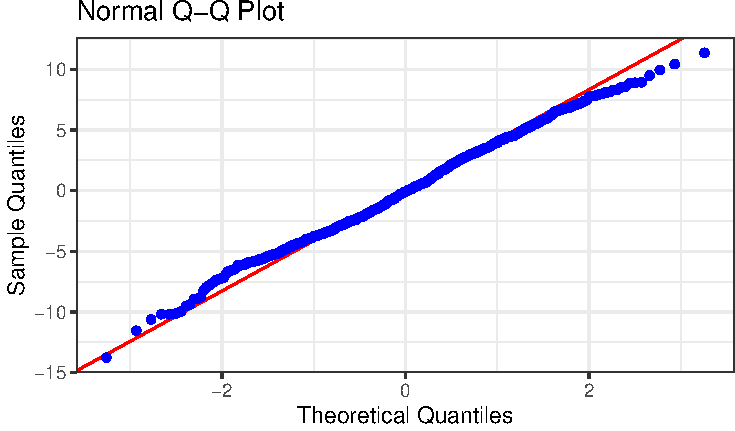
\includegraphics{Appendix_ex_weightloss_files/figure-latex/unnamed-chunk-74-1} \hfill{}

\caption{Residual Diagnostics, Assess Normality of the Conditional Distribution of Weight Loss, QQ Plot}\label{fig:unnamed-chunk-74}
\end{figure}

\begin{Shaded}
\begin{Highlighting}[]
\NormalTok{olsrr}\SpecialCharTok{::}\FunctionTok{ols\_plot\_resid\_hist}\NormalTok{(fit\_2)}
\end{Highlighting}
\end{Shaded}

\begin{figure}[hb]

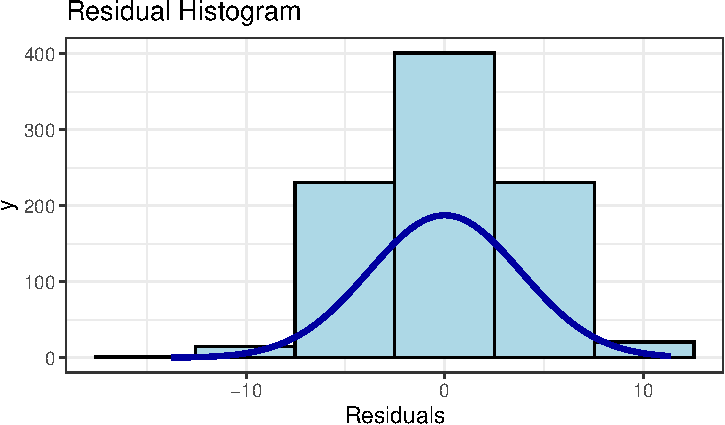
\includegraphics{Appendix_ex_weightloss_files/figure-latex/unnamed-chunk-75-1} \hfill{}

\caption{Residual Diagnostics, Assess Normality of the Conditional Distribution of Weight Loss, Histogram}\label{fig:unnamed-chunk-75}
\end{figure}

\clearpage

It is a scatter plot of residuals on the y axis and fitted values on the
x axis to detect non-linearity, unequal error variances, and outliers.

Characteristics of a well behaved residual vs fitted plot:

\begin{itemize}
\item
  The residuals \textbf{spread randomly} around the 0 line indicating
  that the relationship is linear.
\item
  The residuals form an \textbf{approximate horizontal band} around the
  0 line indicating homogeneity of error variance.
\item
  No one residual is \textbf{visibly away from} the random pattern of
  the residuals indicating that there are no outliers.
\end{itemize}

\begin{Shaded}
\begin{Highlighting}[]
\NormalTok{olsrr}\SpecialCharTok{::}\FunctionTok{ols\_plot\_resid\_fit}\NormalTok{(fit\_2)}
\end{Highlighting}
\end{Shaded}

\begin{figure}[hb]

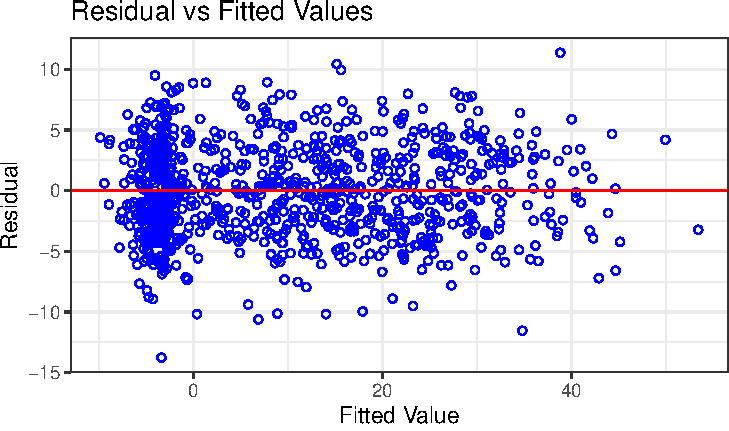
\includegraphics{Appendix_ex_weightloss_files/figure-latex/unnamed-chunk-76-1} \hfill{}

\caption{Residual Diagnostics, Assess Various Assumptions of Regression, scatterplot}\label{fig:unnamed-chunk-76}
\end{figure}

\clearpage

Cook's distance was introduced by American statistician R Dennis Cook in
1977. It is used to \textbf{identify influential data points}. It
depends on both the residual and leverage i.e it takes it account both
the x value and y value of the observation. A data point having a large
cook's d indicates that the data point strongly influences the fitted
values.

\begin{Shaded}
\begin{Highlighting}[]
\NormalTok{olsrr}\SpecialCharTok{::}\FunctionTok{ols\_plot\_cooksd\_chart}\NormalTok{(fit\_2)}
\end{Highlighting}
\end{Shaded}

\begin{figure}[hb]

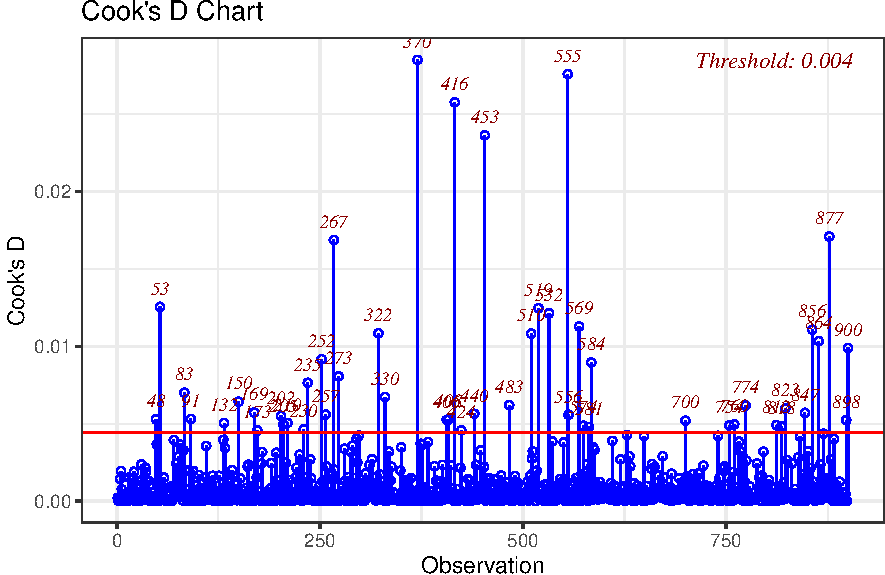
\includegraphics{Appendix_ex_weightloss_files/figure-latex/unnamed-chunk-77-1} \hfill{}

\caption{Residual Diagnostics, Identiry Influential Data Points, Cook's D Chart}\label{fig:unnamed-chunk-77}
\end{figure}

\clearpage

\hypertarget{final-model}{%
\subsection{Final Model}\label{final-model}}

\hypertarget{anlaysis-of-variance}{%
\subsubsection{Anlaysis of Variance}\label{anlaysis-of-variance}}

\begin{Shaded}
\begin{Highlighting}[]
\NormalTok{tab\_lm\_aov }\OtherTok{\textless{}{-}} \FunctionTok{anova}\NormalTok{(fit\_2) }\SpecialCharTok{\%\textgreater{}\%} 
  \FunctionTok{data.frame}\NormalTok{() }\SpecialCharTok{\%\textgreater{}\%}
\NormalTok{  tibble}\SpecialCharTok{::}\FunctionTok{rownames\_to\_column}\NormalTok{() }\SpecialCharTok{\%\textgreater{}\%} 
\NormalTok{  dplyr}\SpecialCharTok{::}\FunctionTok{select}\NormalTok{(}\StringTok{"Model Term"} \OtherTok{=}\NormalTok{ rowname, }
                \AttributeTok{MS =}\NormalTok{ Mean.Sq,}
                \AttributeTok{df =}\NormalTok{ Df,}
                \AttributeTok{F =}\NormalTok{ F.value,}
                \AttributeTok{p =}\NormalTok{ Pr..F.) }\SpecialCharTok{\%\textgreater{}\%} 
\NormalTok{  dplyr}\SpecialCharTok{::}\FunctionTok{mutate}\NormalTok{(}\AttributeTok{p =}\NormalTok{ apaSupp}\SpecialCharTok{::}\FunctionTok{p\_num}\NormalTok{(p)) }\SpecialCharTok{\%\textgreater{}\%} 
\NormalTok{  dplyr}\SpecialCharTok{::}\FunctionTok{mutate\_if}\NormalTok{(is.double, apaSupp}\SpecialCharTok{::}\NormalTok{apa2) }\SpecialCharTok{\%\textgreater{}\%} 
\NormalTok{  flextable}\SpecialCharTok{::}\FunctionTok{flextable}\NormalTok{() }\SpecialCharTok{\%\textgreater{}\%} 
\NormalTok{  flextable}\SpecialCharTok{::}\FunctionTok{set\_caption}\NormalTok{(}\StringTok{"Final Regression Model for Weight Loss, Analysis of Variance and Significance of All Terms"}\NormalTok{)}

\NormalTok{tab\_lm\_aov}
\end{Highlighting}
\end{Shaded}

\global\setlength{\Oldarrayrulewidth}{\arrayrulewidth}

\global\setlength{\Oldtabcolsep}{\tabcolsep}

\setlength{\tabcolsep}{2pt}

\renewcommand*{\arraystretch}{1.5}



\providecommand{\ascline}[3]{\noalign{\global\arrayrulewidth #1}\arrayrulecolor[HTML]{#2}\cline{#3}}

\begin{longtable}[l]{|p{0.75in}|p{0.75in}|p{0.75in}|p{0.75in}|p{0.75in}}

\caption{Final\ Regression\ Model\ for\ Weight\ Loss,\ Analysis\ of\ Variance\ and\ Significance\ of\ All\ Terms}\\

\ascline{0.75pt}{000000}{1-5}

\multicolumn{1}{>{\centering}m{\dimexpr 0.75in+0\tabcolsep}}{\textcolor[HTML]{000000}{\fontsize{10}{20}\selectfont{\global\setmainfont{Times New Roman}{Model\ Term}}}} & \multicolumn{1}{>{\centering}m{\dimexpr 0.75in+0\tabcolsep}}{\textcolor[HTML]{000000}{\fontsize{10}{20}\selectfont{\global\setmainfont{Times New Roman}{MS}}}} & \multicolumn{1}{>{\centering}m{\dimexpr 0.75in+0\tabcolsep}}{\textcolor[HTML]{000000}{\fontsize{10}{20}\selectfont{\global\setmainfont{Times New Roman}{df}}}} & \multicolumn{1}{>{\centering}m{\dimexpr 0.75in+0\tabcolsep}}{\textcolor[HTML]{000000}{\fontsize{10}{20}\selectfont{\global\setmainfont{Times New Roman}{F}}}} & \multicolumn{1}{>{\centering}m{\dimexpr 0.75in+0\tabcolsep}}{\textcolor[HTML]{000000}{\fontsize{10}{20}\selectfont{\global\setmainfont{Times New Roman}{p}}}} \\

\ascline{0.75pt}{000000}{1-5}\endfirsthead \caption[]{Final\ Regression\ Model\ for\ Weight\ Loss,\ Analysis\ of\ Variance\ and\ Significance\ of\ All\ Terms}\\

\ascline{0.75pt}{000000}{1-5}

\multicolumn{1}{>{\centering}m{\dimexpr 0.75in+0\tabcolsep}}{\textcolor[HTML]{000000}{\fontsize{10}{20}\selectfont{\global\setmainfont{Times New Roman}{Model\ Term}}}} & \multicolumn{1}{>{\centering}m{\dimexpr 0.75in+0\tabcolsep}}{\textcolor[HTML]{000000}{\fontsize{10}{20}\selectfont{\global\setmainfont{Times New Roman}{MS}}}} & \multicolumn{1}{>{\centering}m{\dimexpr 0.75in+0\tabcolsep}}{\textcolor[HTML]{000000}{\fontsize{10}{20}\selectfont{\global\setmainfont{Times New Roman}{df}}}} & \multicolumn{1}{>{\centering}m{\dimexpr 0.75in+0\tabcolsep}}{\textcolor[HTML]{000000}{\fontsize{10}{20}\selectfont{\global\setmainfont{Times New Roman}{F}}}} & \multicolumn{1}{>{\centering}m{\dimexpr 0.75in+0\tabcolsep}}{\textcolor[HTML]{000000}{\fontsize{10}{20}\selectfont{\global\setmainfont{Times New Roman}{p}}}} \\

\ascline{0.75pt}{000000}{1-5}\endhead



\multicolumn{1}{>{\centering}m{\dimexpr 0.75in+0\tabcolsep}}{\textcolor[HTML]{000000}{\fontsize{10}{20}\selectfont{\global\setmainfont{Times New Roman}{prog}}}} & \multicolumn{1}{>{\centering}m{\dimexpr 0.75in+0\tabcolsep}}{\textcolor[HTML]{000000}{\fontsize{10}{20}\selectfont{\global\setmainfont{Times New Roman}{66638.60}}}} & \multicolumn{1}{>{\centering}m{\dimexpr 0.75in+0\tabcolsep}}{\textcolor[HTML]{000000}{\fontsize{10}{20}\selectfont{\global\setmainfont{Times New Roman}{2}}}} & \multicolumn{1}{>{\centering}m{\dimexpr 0.75in+0\tabcolsep}}{\textcolor[HTML]{000000}{\fontsize{10}{20}\selectfont{\global\setmainfont{Times New Roman}{4467.31}}}} & \multicolumn{1}{>{\centering}m{\dimexpr 0.75in+0\tabcolsep}}{\textcolor[HTML]{000000}{\fontsize{10}{20}\selectfont{\global\setmainfont{Times New Roman}{<\ .001\ ***}}}} \\





\multicolumn{1}{>{\centering}m{\dimexpr 0.75in+0\tabcolsep}}{\textcolor[HTML]{000000}{\fontsize{10}{20}\selectfont{\global\setmainfont{Times New Roman}{hours}}}} & \multicolumn{1}{>{\centering}m{\dimexpr 0.75in+0\tabcolsep}}{\textcolor[HTML]{000000}{\fontsize{10}{20}\selectfont{\global\setmainfont{Times New Roman}{\ 2344.49}}}} & \multicolumn{1}{>{\centering}m{\dimexpr 0.75in+0\tabcolsep}}{\textcolor[HTML]{000000}{\fontsize{10}{20}\selectfont{\global\setmainfont{Times New Roman}{1}}}} & \multicolumn{1}{>{\centering}m{\dimexpr 0.75in+0\tabcolsep}}{\textcolor[HTML]{000000}{\fontsize{10}{20}\selectfont{\global\setmainfont{Times New Roman}{\ 157.17}}}} & \multicolumn{1}{>{\centering}m{\dimexpr 0.75in+0\tabcolsep}}{\textcolor[HTML]{000000}{\fontsize{10}{20}\selectfont{\global\setmainfont{Times New Roman}{<\ .001\ ***}}}} \\





\multicolumn{1}{>{\centering}m{\dimexpr 0.75in+0\tabcolsep}}{\textcolor[HTML]{000000}{\fontsize{10}{20}\selectfont{\global\setmainfont{Times New Roman}{gender}}}} & \multicolumn{1}{>{\centering}m{\dimexpr 0.75in+0\tabcolsep}}{\textcolor[HTML]{000000}{\fontsize{10}{20}\selectfont{\global\setmainfont{Times New Roman}{\ \ \ \ 2.14}}}} & \multicolumn{1}{>{\centering}m{\dimexpr 0.75in+0\tabcolsep}}{\textcolor[HTML]{000000}{\fontsize{10}{20}\selectfont{\global\setmainfont{Times New Roman}{1}}}} & \multicolumn{1}{>{\centering}m{\dimexpr 0.75in+0\tabcolsep}}{\textcolor[HTML]{000000}{\fontsize{10}{20}\selectfont{\global\setmainfont{Times New Roman}{\ \ \ 0.14}}}} & \multicolumn{1}{>{\centering}m{\dimexpr 0.75in+0\tabcolsep}}{\textcolor[HTML]{000000}{\fontsize{10}{20}\selectfont{\global\setmainfont{Times New Roman}{.705}}}} \\





\multicolumn{1}{>{\centering}m{\dimexpr 0.75in+0\tabcolsep}}{\textcolor[HTML]{000000}{\fontsize{10}{20}\selectfont{\global\setmainfont{Times New Roman}{effort}}}} & \multicolumn{1}{>{\centering}m{\dimexpr 0.75in+0\tabcolsep}}{\textcolor[HTML]{000000}{\fontsize{10}{20}\selectfont{\global\setmainfont{Times New Roman}{10046.72}}}} & \multicolumn{1}{>{\centering}m{\dimexpr 0.75in+0\tabcolsep}}{\textcolor[HTML]{000000}{\fontsize{10}{20}\selectfont{\global\setmainfont{Times New Roman}{1}}}} & \multicolumn{1}{>{\centering}m{\dimexpr 0.75in+0\tabcolsep}}{\textcolor[HTML]{000000}{\fontsize{10}{20}\selectfont{\global\setmainfont{Times New Roman}{\ 673.51}}}} & \multicolumn{1}{>{\centering}m{\dimexpr 0.75in+0\tabcolsep}}{\textcolor[HTML]{000000}{\fontsize{10}{20}\selectfont{\global\setmainfont{Times New Roman}{<\ .001\ ***}}}} \\





\multicolumn{1}{>{\centering}m{\dimexpr 0.75in+0\tabcolsep}}{\textcolor[HTML]{000000}{\fontsize{10}{20}\selectfont{\global\setmainfont{Times New Roman}{prog:hours}}}} & \multicolumn{1}{>{\centering}m{\dimexpr 0.75in+0\tabcolsep}}{\textcolor[HTML]{000000}{\fontsize{10}{20}\selectfont{\global\setmainfont{Times New Roman}{\ 2748.38}}}} & \multicolumn{1}{>{\centering}m{\dimexpr 0.75in+0\tabcolsep}}{\textcolor[HTML]{000000}{\fontsize{10}{20}\selectfont{\global\setmainfont{Times New Roman}{2}}}} & \multicolumn{1}{>{\centering}m{\dimexpr 0.75in+0\tabcolsep}}{\textcolor[HTML]{000000}{\fontsize{10}{20}\selectfont{\global\setmainfont{Times New Roman}{\ 184.25}}}} & \multicolumn{1}{>{\centering}m{\dimexpr 0.75in+0\tabcolsep}}{\textcolor[HTML]{000000}{\fontsize{10}{20}\selectfont{\global\setmainfont{Times New Roman}{<\ .001\ ***}}}} \\





\multicolumn{1}{>{\centering}m{\dimexpr 0.75in+0\tabcolsep}}{\textcolor[HTML]{000000}{\fontsize{10}{20}\selectfont{\global\setmainfont{Times New Roman}{prog:gender}}}} & \multicolumn{1}{>{\centering}m{\dimexpr 0.75in+0\tabcolsep}}{\textcolor[HTML]{000000}{\fontsize{10}{20}\selectfont{\global\setmainfont{Times New Roman}{\ 3392.35}}}} & \multicolumn{1}{>{\centering}m{\dimexpr 0.75in+0\tabcolsep}}{\textcolor[HTML]{000000}{\fontsize{10}{20}\selectfont{\global\setmainfont{Times New Roman}{2}}}} & \multicolumn{1}{>{\centering}m{\dimexpr 0.75in+0\tabcolsep}}{\textcolor[HTML]{000000}{\fontsize{10}{20}\selectfont{\global\setmainfont{Times New Roman}{\ 227.42}}}} & \multicolumn{1}{>{\centering}m{\dimexpr 0.75in+0\tabcolsep}}{\textcolor[HTML]{000000}{\fontsize{10}{20}\selectfont{\global\setmainfont{Times New Roman}{<\ .001\ ***}}}} \\





\multicolumn{1}{>{\centering}m{\dimexpr 0.75in+0\tabcolsep}}{\textcolor[HTML]{000000}{\fontsize{10}{20}\selectfont{\global\setmainfont{Times New Roman}{hours:gender}}}} & \multicolumn{1}{>{\centering}m{\dimexpr 0.75in+0\tabcolsep}}{\textcolor[HTML]{000000}{\fontsize{10}{20}\selectfont{\global\setmainfont{Times New Roman}{\ \ \ 77.31}}}} & \multicolumn{1}{>{\centering}m{\dimexpr 0.75in+0\tabcolsep}}{\textcolor[HTML]{000000}{\fontsize{10}{20}\selectfont{\global\setmainfont{Times New Roman}{1}}}} & \multicolumn{1}{>{\centering}m{\dimexpr 0.75in+0\tabcolsep}}{\textcolor[HTML]{000000}{\fontsize{10}{20}\selectfont{\global\setmainfont{Times New Roman}{\ \ \ 5.18}}}} & \multicolumn{1}{>{\centering}m{\dimexpr 0.75in+0\tabcolsep}}{\textcolor[HTML]{000000}{\fontsize{10}{20}\selectfont{\global\setmainfont{Times New Roman}{.023\ *}}}} \\





\multicolumn{1}{>{\centering}m{\dimexpr 0.75in+0\tabcolsep}}{\textcolor[HTML]{000000}{\fontsize{10}{20}\selectfont{\global\setmainfont{Times New Roman}{prog:effort}}}} & \multicolumn{1}{>{\centering}m{\dimexpr 0.75in+0\tabcolsep}}{\textcolor[HTML]{000000}{\fontsize{10}{20}\selectfont{\global\setmainfont{Times New Roman}{\ 2684.32}}}} & \multicolumn{1}{>{\centering}m{\dimexpr 0.75in+0\tabcolsep}}{\textcolor[HTML]{000000}{\fontsize{10}{20}\selectfont{\global\setmainfont{Times New Roman}{2}}}} & \multicolumn{1}{>{\centering}m{\dimexpr 0.75in+0\tabcolsep}}{\textcolor[HTML]{000000}{\fontsize{10}{20}\selectfont{\global\setmainfont{Times New Roman}{\ 179.95}}}} & \multicolumn{1}{>{\centering}m{\dimexpr 0.75in+0\tabcolsep}}{\textcolor[HTML]{000000}{\fontsize{10}{20}\selectfont{\global\setmainfont{Times New Roman}{<\ .001\ ***}}}} \\





\multicolumn{1}{>{\centering}m{\dimexpr 0.75in+0\tabcolsep}}{\textcolor[HTML]{000000}{\fontsize{10}{20}\selectfont{\global\setmainfont{Times New Roman}{hours:effort}}}} & \multicolumn{1}{>{\centering}m{\dimexpr 0.75in+0\tabcolsep}}{\textcolor[HTML]{000000}{\fontsize{10}{20}\selectfont{\global\setmainfont{Times New Roman}{\ \ 766.94}}}} & \multicolumn{1}{>{\centering}m{\dimexpr 0.75in+0\tabcolsep}}{\textcolor[HTML]{000000}{\fontsize{10}{20}\selectfont{\global\setmainfont{Times New Roman}{1}}}} & \multicolumn{1}{>{\centering}m{\dimexpr 0.75in+0\tabcolsep}}{\textcolor[HTML]{000000}{\fontsize{10}{20}\selectfont{\global\setmainfont{Times New Roman}{\ \ 51.41}}}} & \multicolumn{1}{>{\centering}m{\dimexpr 0.75in+0\tabcolsep}}{\textcolor[HTML]{000000}{\fontsize{10}{20}\selectfont{\global\setmainfont{Times New Roman}{<\ .001\ ***}}}} \\





\multicolumn{1}{>{\centering}m{\dimexpr 0.75in+0\tabcolsep}}{\textcolor[HTML]{000000}{\fontsize{10}{20}\selectfont{\global\setmainfont{Times New Roman}{prog:hours:gender}}}} & \multicolumn{1}{>{\centering}m{\dimexpr 0.75in+0\tabcolsep}}{\textcolor[HTML]{000000}{\fontsize{10}{20}\selectfont{\global\setmainfont{Times New Roman}{\ \ 545.54}}}} & \multicolumn{1}{>{\centering}m{\dimexpr 0.75in+0\tabcolsep}}{\textcolor[HTML]{000000}{\fontsize{10}{20}\selectfont{\global\setmainfont{Times New Roman}{2}}}} & \multicolumn{1}{>{\centering}m{\dimexpr 0.75in+0\tabcolsep}}{\textcolor[HTML]{000000}{\fontsize{10}{20}\selectfont{\global\setmainfont{Times New Roman}{\ \ 36.57}}}} & \multicolumn{1}{>{\centering}m{\dimexpr 0.75in+0\tabcolsep}}{\textcolor[HTML]{000000}{\fontsize{10}{20}\selectfont{\global\setmainfont{Times New Roman}{<\ .001\ ***}}}} \\





\multicolumn{1}{>{\centering}m{\dimexpr 0.75in+0\tabcolsep}}{\textcolor[HTML]{000000}{\fontsize{10}{20}\selectfont{\global\setmainfont{Times New Roman}{prog:hours:effort}}}} & \multicolumn{1}{>{\centering}m{\dimexpr 0.75in+0\tabcolsep}}{\textcolor[HTML]{000000}{\fontsize{10}{20}\selectfont{\global\setmainfont{Times New Roman}{\ \ 161.74}}}} & \multicolumn{1}{>{\centering}m{\dimexpr 0.75in+0\tabcolsep}}{\textcolor[HTML]{000000}{\fontsize{10}{20}\selectfont{\global\setmainfont{Times New Roman}{2}}}} & \multicolumn{1}{>{\centering}m{\dimexpr 0.75in+0\tabcolsep}}{\textcolor[HTML]{000000}{\fontsize{10}{20}\selectfont{\global\setmainfont{Times New Roman}{\ \ 10.84}}}} & \multicolumn{1}{>{\centering}m{\dimexpr 0.75in+0\tabcolsep}}{\textcolor[HTML]{000000}{\fontsize{10}{20}\selectfont{\global\setmainfont{Times New Roman}{<\ .001\ ***}}}} \\





\multicolumn{1}{>{\centering}m{\dimexpr 0.75in+0\tabcolsep}}{\textcolor[HTML]{000000}{\fontsize{10}{20}\selectfont{\global\setmainfont{Times New Roman}{Residuals}}}} & \multicolumn{1}{>{\centering}m{\dimexpr 0.75in+0\tabcolsep}}{\textcolor[HTML]{000000}{\fontsize{10}{20}\selectfont{\global\setmainfont{Times New Roman}{\ \ \ 14.92}}}} & \multicolumn{1}{>{\centering}m{\dimexpr 0.75in+0\tabcolsep}}{\textcolor[HTML]{000000}{\fontsize{10}{20}\selectfont{\global\setmainfont{Times New Roman}{882}}}} & \multicolumn{1}{>{\centering}m{\dimexpr 0.75in+0\tabcolsep}}{\textcolor[HTML]{000000}{\fontsize{10}{20}\selectfont{\global\setmainfont{Times New Roman}{\ \ \ \ \ NA}}}} & \multicolumn{1}{>{\centering}m{\dimexpr 0.75in+0\tabcolsep}}{\textcolor[HTML]{000000}{\fontsize{10}{20}\selectfont{\global\setmainfont{Times New Roman}{}}}} \\

\ascline{0.75pt}{000000}{1-5}



\end{longtable}



\arrayrulecolor[HTML]{000000}

\global\setlength{\arrayrulewidth}{\Oldarrayrulewidth}

\global\setlength{\tabcolsep}{\Oldtabcolsep}

\renewcommand*{\arraystretch}{1}

\clearpage

\hypertarget{parameter-estimates}{%
\subsubsection{Parameter Estimates}\label{parameter-estimates}}

\begin{Shaded}
\begin{Highlighting}[]
\CommentTok{\# texreg::knitreg(fit\_2,}
\CommentTok{\#                 custom.model.names = "Weight Loss, pounds",}
\CommentTok{\#                 single.row = TRUE,}
\CommentTok{\#                 caption = "Parameter Estimates of Final Regression Models for Weight Loss")}
\end{Highlighting}
\end{Shaded}

\clearpage

\hypertarget{simple-slopes-analysis}{%
\subsubsection{Simple Slopes Analysis}\label{simple-slopes-analysis}}

\begin{Shaded}
\begin{Highlighting}[]
\NormalTok{tab\_simpslopes }\OtherTok{\textless{}{-}}\NormalTok{ interactions}\SpecialCharTok{::}\FunctionTok{sim\_slopes}\NormalTok{(}\AttributeTok{model =}\NormalTok{ fit\_2,}
                                           \AttributeTok{pred =}\NormalTok{ hours,}
                                           \AttributeTok{modx =}\NormalTok{ prog,}
                                           \AttributeTok{mod2 =}\NormalTok{ gender) }\SpecialCharTok{\%\textgreater{}\%} 
\NormalTok{  broom}\SpecialCharTok{::}\FunctionTok{tidy}\NormalTok{() }\SpecialCharTok{\%\textgreater{}\%} 
\NormalTok{  dplyr}\SpecialCharTok{::}\FunctionTok{select}\NormalTok{(}\AttributeTok{Gender =}\NormalTok{ mod2.value,}
                \AttributeTok{Program =}\NormalTok{ modx.value,}
                \AttributeTok{b =}\NormalTok{ estimate,}
                \AttributeTok{SE =}\NormalTok{ std.error,}
                \AttributeTok{CI\_lo =}\NormalTok{ conf.low,}
                \AttributeTok{CI\_hi =}\NormalTok{ conf.high,}
                \AttributeTok{p =}\NormalTok{ p.value) }\SpecialCharTok{\%\textgreater{}\%} 
\NormalTok{  dplyr}\SpecialCharTok{::}\FunctionTok{mutate}\NormalTok{(}\FunctionTok{across}\NormalTok{(}\FunctionTok{c}\NormalTok{(b, SE, p, CI\_lo, CI\_hi),}
\NormalTok{                       as.numeric)) }\SpecialCharTok{\%\textgreater{}\%} 
\NormalTok{  dplyr}\SpecialCharTok{::}\FunctionTok{mutate}\NormalTok{(}\AttributeTok{p =}\NormalTok{ apaSupp}\SpecialCharTok{::}\FunctionTok{p\_num}\NormalTok{(p)) }\SpecialCharTok{\%\textgreater{}\%} 
\NormalTok{  dplyr}\SpecialCharTok{::}\FunctionTok{mutate\_if}\NormalTok{(is.numeric, apaSupp}\SpecialCharTok{::}\NormalTok{apa2) }\SpecialCharTok{\%\textgreater{}\%} 
\NormalTok{  flextable}\SpecialCharTok{::}\FunctionTok{flextable}\NormalTok{()}\SpecialCharTok{\%\textgreater{}\%} 
\NormalTok{  flextable}\SpecialCharTok{::}\FunctionTok{set\_caption}\NormalTok{(}\StringTok{"Simple Slopes Analysis for Weight Loss by Time Spent in each Program by Gender, Collapsed Across Effort"}\NormalTok{)}

\NormalTok{tab\_simpslopes}
\end{Highlighting}
\end{Shaded}

\global\setlength{\Oldarrayrulewidth}{\arrayrulewidth}

\global\setlength{\Oldtabcolsep}{\tabcolsep}

\setlength{\tabcolsep}{2pt}

\renewcommand*{\arraystretch}{1.5}



\providecommand{\ascline}[3]{\noalign{\global\arrayrulewidth #1}\arrayrulecolor[HTML]{#2}\cline{#3}}

\begin{longtable}[l]{|p{0.75in}|p{0.75in}|p{0.75in}|p{0.75in}|p{0.75in}|p{0.75in}|p{0.75in}}

\caption{Simple\ Slopes\ Analysis\ for\ Weight\ Loss\ by\ Time\ Spent\ in\ each\ Program\ by\ Gender,\ Collapsed\ Across\ Effort}\\

\ascline{0.75pt}{000000}{1-7}

\multicolumn{1}{>{\centering}m{\dimexpr 0.75in+0\tabcolsep}}{\textcolor[HTML]{000000}{\fontsize{10}{20}\selectfont{\global\setmainfont{Times New Roman}{Gender}}}} & \multicolumn{1}{>{\centering}m{\dimexpr 0.75in+0\tabcolsep}}{\textcolor[HTML]{000000}{\fontsize{10}{20}\selectfont{\global\setmainfont{Times New Roman}{Program}}}} & \multicolumn{1}{>{\centering}m{\dimexpr 0.75in+0\tabcolsep}}{\textcolor[HTML]{000000}{\fontsize{10}{20}\selectfont{\global\setmainfont{Times New Roman}{b}}}} & \multicolumn{1}{>{\centering}m{\dimexpr 0.75in+0\tabcolsep}}{\textcolor[HTML]{000000}{\fontsize{10}{20}\selectfont{\global\setmainfont{Times New Roman}{SE}}}} & \multicolumn{1}{>{\centering}m{\dimexpr 0.75in+0\tabcolsep}}{\textcolor[HTML]{000000}{\fontsize{10}{20}\selectfont{\global\setmainfont{Times New Roman}{CI\_lo}}}} & \multicolumn{1}{>{\centering}m{\dimexpr 0.75in+0\tabcolsep}}{\textcolor[HTML]{000000}{\fontsize{10}{20}\selectfont{\global\setmainfont{Times New Roman}{CI\_hi}}}} & \multicolumn{1}{>{\centering}m{\dimexpr 0.75in+0\tabcolsep}}{\textcolor[HTML]{000000}{\fontsize{10}{20}\selectfont{\global\setmainfont{Times New Roman}{p}}}} \\

\ascline{0.75pt}{000000}{1-7}\endfirsthead \caption[]{Simple\ Slopes\ Analysis\ for\ Weight\ Loss\ by\ Time\ Spent\ in\ each\ Program\ by\ Gender,\ Collapsed\ Across\ Effort}\\

\ascline{0.75pt}{000000}{1-7}

\multicolumn{1}{>{\centering}m{\dimexpr 0.75in+0\tabcolsep}}{\textcolor[HTML]{000000}{\fontsize{10}{20}\selectfont{\global\setmainfont{Times New Roman}{Gender}}}} & \multicolumn{1}{>{\centering}m{\dimexpr 0.75in+0\tabcolsep}}{\textcolor[HTML]{000000}{\fontsize{10}{20}\selectfont{\global\setmainfont{Times New Roman}{Program}}}} & \multicolumn{1}{>{\centering}m{\dimexpr 0.75in+0\tabcolsep}}{\textcolor[HTML]{000000}{\fontsize{10}{20}\selectfont{\global\setmainfont{Times New Roman}{b}}}} & \multicolumn{1}{>{\centering}m{\dimexpr 0.75in+0\tabcolsep}}{\textcolor[HTML]{000000}{\fontsize{10}{20}\selectfont{\global\setmainfont{Times New Roman}{SE}}}} & \multicolumn{1}{>{\centering}m{\dimexpr 0.75in+0\tabcolsep}}{\textcolor[HTML]{000000}{\fontsize{10}{20}\selectfont{\global\setmainfont{Times New Roman}{CI\_lo}}}} & \multicolumn{1}{>{\centering}m{\dimexpr 0.75in+0\tabcolsep}}{\textcolor[HTML]{000000}{\fontsize{10}{20}\selectfont{\global\setmainfont{Times New Roman}{CI\_hi}}}} & \multicolumn{1}{>{\centering}m{\dimexpr 0.75in+0\tabcolsep}}{\textcolor[HTML]{000000}{\fontsize{10}{20}\selectfont{\global\setmainfont{Times New Roman}{p}}}} \\

\ascline{0.75pt}{000000}{1-7}\endhead



\multicolumn{1}{>{\centering}m{\dimexpr 0.75in+0\tabcolsep}}{\textcolor[HTML]{000000}{\fontsize{10}{20}\selectfont{\global\setmainfont{Times New Roman}{Male}}}} & \multicolumn{1}{>{\centering}m{\dimexpr 0.75in+0\tabcolsep}}{\textcolor[HTML]{000000}{\fontsize{10}{20}\selectfont{\global\setmainfont{Times New Roman}{Jogging}}}} & \multicolumn{1}{>{\centering}m{\dimexpr 0.75in+0\tabcolsep}}{\textcolor[HTML]{000000}{\fontsize{10}{20}\selectfont{\global\setmainfont{Times New Roman}{\ 2.68}}}} & \multicolumn{1}{>{\centering}m{\dimexpr 0.75in+0\tabcolsep}}{\textcolor[HTML]{000000}{\fontsize{10}{20}\selectfont{\global\setmainfont{Times New Roman}{0.67}}}} & \multicolumn{1}{>{\centering}m{\dimexpr 0.75in+0\tabcolsep}}{\textcolor[HTML]{000000}{\fontsize{10}{20}\selectfont{\global\setmainfont{Times New Roman}{\ 1.36}}}} & \multicolumn{1}{>{\centering}m{\dimexpr 0.75in+0\tabcolsep}}{\textcolor[HTML]{000000}{\fontsize{10}{20}\selectfont{\global\setmainfont{Times New Roman}{\ 4.01}}}} & \multicolumn{1}{>{\centering}m{\dimexpr 0.75in+0\tabcolsep}}{\textcolor[HTML]{000000}{\fontsize{10}{20}\selectfont{\global\setmainfont{Times New Roman}{<\ .001\ ***}}}} \\





\multicolumn{1}{>{\centering}m{\dimexpr 0.75in+0\tabcolsep}}{\textcolor[HTML]{000000}{\fontsize{10}{20}\selectfont{\global\setmainfont{Times New Roman}{Male}}}} & \multicolumn{1}{>{\centering}m{\dimexpr 0.75in+0\tabcolsep}}{\textcolor[HTML]{000000}{\fontsize{10}{20}\selectfont{\global\setmainfont{Times New Roman}{Swimming}}}} & \multicolumn{1}{>{\centering}m{\dimexpr 0.75in+0\tabcolsep}}{\textcolor[HTML]{000000}{\fontsize{10}{20}\selectfont{\global\setmainfont{Times New Roman}{\ 9.13}}}} & \multicolumn{1}{>{\centering}m{\dimexpr 0.75in+0\tabcolsep}}{\textcolor[HTML]{000000}{\fontsize{10}{20}\selectfont{\global\setmainfont{Times New Roman}{0.66}}}} & \multicolumn{1}{>{\centering}m{\dimexpr 0.75in+0\tabcolsep}}{\textcolor[HTML]{000000}{\fontsize{10}{20}\selectfont{\global\setmainfont{Times New Roman}{\ 7.84}}}} & \multicolumn{1}{>{\centering}m{\dimexpr 0.75in+0\tabcolsep}}{\textcolor[HTML]{000000}{\fontsize{10}{20}\selectfont{\global\setmainfont{Times New Roman}{10.41}}}} & \multicolumn{1}{>{\centering}m{\dimexpr 0.75in+0\tabcolsep}}{\textcolor[HTML]{000000}{\fontsize{10}{20}\selectfont{\global\setmainfont{Times New Roman}{<\ .001\ ***}}}} \\





\multicolumn{1}{>{\centering}m{\dimexpr 0.75in+0\tabcolsep}}{\textcolor[HTML]{000000}{\fontsize{10}{20}\selectfont{\global\setmainfont{Times New Roman}{Male}}}} & \multicolumn{1}{>{\centering}m{\dimexpr 0.75in+0\tabcolsep}}{\textcolor[HTML]{000000}{\fontsize{10}{20}\selectfont{\global\setmainfont{Times New Roman}{Reading}}}} & \multicolumn{1}{>{\centering}m{\dimexpr 0.75in+0\tabcolsep}}{\textcolor[HTML]{000000}{\fontsize{10}{20}\selectfont{\global\setmainfont{Times New Roman}{-3.74}}}} & \multicolumn{1}{>{\centering}m{\dimexpr 0.75in+0\tabcolsep}}{\textcolor[HTML]{000000}{\fontsize{10}{20}\selectfont{\global\setmainfont{Times New Roman}{0.62}}}} & \multicolumn{1}{>{\centering}m{\dimexpr 0.75in+0\tabcolsep}}{\textcolor[HTML]{000000}{\fontsize{10}{20}\selectfont{\global\setmainfont{Times New Roman}{-4.96}}}} & \multicolumn{1}{>{\centering}m{\dimexpr 0.75in+0\tabcolsep}}{\textcolor[HTML]{000000}{\fontsize{10}{20}\selectfont{\global\setmainfont{Times New Roman}{-2.52}}}} & \multicolumn{1}{>{\centering}m{\dimexpr 0.75in+0\tabcolsep}}{\textcolor[HTML]{000000}{\fontsize{10}{20}\selectfont{\global\setmainfont{Times New Roman}{<\ .001\ ***}}}} \\





\multicolumn{1}{>{\centering}m{\dimexpr 0.75in+0\tabcolsep}}{\textcolor[HTML]{000000}{\fontsize{10}{20}\selectfont{\global\setmainfont{Times New Roman}{Female}}}} & \multicolumn{1}{>{\centering}m{\dimexpr 0.75in+0\tabcolsep}}{\textcolor[HTML]{000000}{\fontsize{10}{20}\selectfont{\global\setmainfont{Times New Roman}{Jogging}}}} & \multicolumn{1}{>{\centering}m{\dimexpr 0.75in+0\tabcolsep}}{\textcolor[HTML]{000000}{\fontsize{10}{20}\selectfont{\global\setmainfont{Times New Roman}{\ 9.86}}}} & \multicolumn{1}{>{\centering}m{\dimexpr 0.75in+0\tabcolsep}}{\textcolor[HTML]{000000}{\fontsize{10}{20}\selectfont{\global\setmainfont{Times New Roman}{0.70}}}} & \multicolumn{1}{>{\centering}m{\dimexpr 0.75in+0\tabcolsep}}{\textcolor[HTML]{000000}{\fontsize{10}{20}\selectfont{\global\setmainfont{Times New Roman}{\ 8.49}}}} & \multicolumn{1}{>{\centering}m{\dimexpr 0.75in+0\tabcolsep}}{\textcolor[HTML]{000000}{\fontsize{10}{20}\selectfont{\global\setmainfont{Times New Roman}{11.24}}}} & \multicolumn{1}{>{\centering}m{\dimexpr 0.75in+0\tabcolsep}}{\textcolor[HTML]{000000}{\fontsize{10}{20}\selectfont{\global\setmainfont{Times New Roman}{<\ .001\ ***}}}} \\





\multicolumn{1}{>{\centering}m{\dimexpr 0.75in+0\tabcolsep}}{\textcolor[HTML]{000000}{\fontsize{10}{20}\selectfont{\global\setmainfont{Times New Roman}{Female}}}} & \multicolumn{1}{>{\centering}m{\dimexpr 0.75in+0\tabcolsep}}{\textcolor[HTML]{000000}{\fontsize{10}{20}\selectfont{\global\setmainfont{Times New Roman}{Swimming}}}} & \multicolumn{1}{>{\centering}m{\dimexpr 0.75in+0\tabcolsep}}{\textcolor[HTML]{000000}{\fontsize{10}{20}\selectfont{\global\setmainfont{Times New Roman}{\ 5.15}}}} & \multicolumn{1}{>{\centering}m{\dimexpr 0.75in+0\tabcolsep}}{\textcolor[HTML]{000000}{\fontsize{10}{20}\selectfont{\global\setmainfont{Times New Roman}{0.66}}}} & \multicolumn{1}{>{\centering}m{\dimexpr 0.75in+0\tabcolsep}}{\textcolor[HTML]{000000}{\fontsize{10}{20}\selectfont{\global\setmainfont{Times New Roman}{\ 3.86}}}} & \multicolumn{1}{>{\centering}m{\dimexpr 0.75in+0\tabcolsep}}{\textcolor[HTML]{000000}{\fontsize{10}{20}\selectfont{\global\setmainfont{Times New Roman}{\ 6.44}}}} & \multicolumn{1}{>{\centering}m{\dimexpr 0.75in+0\tabcolsep}}{\textcolor[HTML]{000000}{\fontsize{10}{20}\selectfont{\global\setmainfont{Times New Roman}{<\ .001\ ***}}}} \\





\multicolumn{1}{>{\centering}m{\dimexpr 0.75in+0\tabcolsep}}{\textcolor[HTML]{000000}{\fontsize{10}{20}\selectfont{\global\setmainfont{Times New Roman}{Female}}}} & \multicolumn{1}{>{\centering}m{\dimexpr 0.75in+0\tabcolsep}}{\textcolor[HTML]{000000}{\fontsize{10}{20}\selectfont{\global\setmainfont{Times New Roman}{Reading}}}} & \multicolumn{1}{>{\centering}m{\dimexpr 0.75in+0\tabcolsep}}{\textcolor[HTML]{000000}{\fontsize{10}{20}\selectfont{\global\setmainfont{Times New Roman}{-2.19}}}} & \multicolumn{1}{>{\centering}m{\dimexpr 0.75in+0\tabcolsep}}{\textcolor[HTML]{000000}{\fontsize{10}{20}\selectfont{\global\setmainfont{Times New Roman}{0.58}}}} & \multicolumn{1}{>{\centering}m{\dimexpr 0.75in+0\tabcolsep}}{\textcolor[HTML]{000000}{\fontsize{10}{20}\selectfont{\global\setmainfont{Times New Roman}{-3.32}}}} & \multicolumn{1}{>{\centering}m{\dimexpr 0.75in+0\tabcolsep}}{\textcolor[HTML]{000000}{\fontsize{10}{20}\selectfont{\global\setmainfont{Times New Roman}{-1.06}}}} & \multicolumn{1}{>{\centering}m{\dimexpr 0.75in+0\tabcolsep}}{\textcolor[HTML]{000000}{\fontsize{10}{20}\selectfont{\global\setmainfont{Times New Roman}{<\ .001\ ***}}}} \\

\ascline{0.75pt}{000000}{1-7}



\end{longtable}



\arrayrulecolor[HTML]{000000}

\global\setlength{\arrayrulewidth}{\Oldarrayrulewidth}

\global\setlength{\tabcolsep}{\Oldtabcolsep}

\renewcommand*{\arraystretch}{1}

\clearpage

\hypertarget{visualization}{%
\subsubsection{Visualization}\label{visualization}}

\begin{Shaded}
\begin{Highlighting}[]
\NormalTok{effects}\SpecialCharTok{::}\FunctionTok{Effect}\NormalTok{(}\AttributeTok{mod =}\NormalTok{ fit\_2,}
                \AttributeTok{focal.predictors =} \FunctionTok{c}\NormalTok{(}\StringTok{"prog"}\NormalTok{, }\StringTok{"hours"}\NormalTok{, }
                                     \StringTok{"gender"}\NormalTok{, }\StringTok{"effort"}\NormalTok{),}
                \AttributeTok{xlevels =} \FunctionTok{list}\NormalTok{(}\AttributeTok{hours =} \FunctionTok{seq}\NormalTok{(}\AttributeTok{from =} \DecValTok{0}\NormalTok{,}
                                           \AttributeTok{to =} \DecValTok{4}\NormalTok{,}
                                           \AttributeTok{by =}\NormalTok{ .}\DecValTok{1}\NormalTok{),}
                               \AttributeTok{effort =} \FunctionTok{c}\NormalTok{(}\FloatTok{26.26}\NormalTok{, }\FloatTok{29.66}\NormalTok{, }\FloatTok{33.10}\NormalTok{))) }\SpecialCharTok{\%\textgreater{}\%} 
  \FunctionTok{data.frame}\NormalTok{() }\SpecialCharTok{\%\textgreater{}\%} 
\NormalTok{  dplyr}\SpecialCharTok{::}\FunctionTok{mutate}\NormalTok{(}\AttributeTok{effort =}\NormalTok{ effort }\SpecialCharTok{\%\textgreater{}\%} 
                  \FunctionTok{factor}\NormalTok{(}\AttributeTok{levels =} \FunctionTok{c}\NormalTok{(}\FloatTok{26.26}\NormalTok{, }\FloatTok{29.66}\NormalTok{,}\FloatTok{33.10}\NormalTok{),}
                         \AttributeTok{labels =} \FunctionTok{c}\NormalTok{(}\StringTok{"Low Effort (Q1)"}\NormalTok{,}
                                    \StringTok{"Avg Effort (Mean)"}\NormalTok{,}
                                    \StringTok{"High Effort (Q3)"}\NormalTok{))) }\SpecialCharTok{\%\textgreater{}\%} 
  \FunctionTok{ggplot}\NormalTok{(}\FunctionTok{aes}\NormalTok{(}\AttributeTok{x =}\NormalTok{ hours,}
             \AttributeTok{y =}\NormalTok{ fit,}
             \AttributeTok{group =}\NormalTok{ prog)) }\SpecialCharTok{+}
  \FunctionTok{geom\_ribbon}\NormalTok{(}\FunctionTok{aes}\NormalTok{(}\AttributeTok{ymin =}\NormalTok{ lower,}
                  \AttributeTok{ymax =}\NormalTok{ upper,}
                  \AttributeTok{fill =}\NormalTok{ prog),}
              \AttributeTok{alpha =}\NormalTok{ .}\DecValTok{3}\NormalTok{) }\SpecialCharTok{+}
  \FunctionTok{geom\_line}\NormalTok{(}\FunctionTok{aes}\NormalTok{(}\AttributeTok{linetype =}\NormalTok{ prog)) }\SpecialCharTok{+}
  \FunctionTok{theme\_bw}\NormalTok{() }\SpecialCharTok{+}
  \FunctionTok{facet\_grid}\NormalTok{(gender }\SpecialCharTok{\textasciitilde{}}\NormalTok{ effort) }\SpecialCharTok{+}
  \FunctionTok{geom\_hline}\NormalTok{(}\AttributeTok{yintercept =} \DecValTok{0}\NormalTok{, }\AttributeTok{color =} \StringTok{"black"}\NormalTok{) }\SpecialCharTok{+}
  \FunctionTok{scale\_linetype\_manual}\NormalTok{(}\AttributeTok{values =} \FunctionTok{c}\NormalTok{(}\StringTok{"solid"}\NormalTok{, }\StringTok{"longdash"}\NormalTok{, }\StringTok{"dotted"}\NormalTok{)) }\SpecialCharTok{+}
  \FunctionTok{labs}\NormalTok{(}\AttributeTok{x =} \StringTok{"Program Time, hours/week"}\NormalTok{,}
       \AttributeTok{y =} \StringTok{"Weight Loss, pounds}\SpecialCharTok{\textbackslash{}n}\StringTok{Estimated Marginal Mean"}\NormalTok{,}
       \AttributeTok{linetype =} \ConstantTok{NULL}\NormalTok{,}
       \AttributeTok{color =} \ConstantTok{NULL}\NormalTok{,}
       \AttributeTok{fill =} \ConstantTok{NULL}\NormalTok{)  }\SpecialCharTok{+}
  \FunctionTok{theme}\NormalTok{(}\AttributeTok{legend.position =} \StringTok{"bottom"}\NormalTok{,}
        \AttributeTok{legend.key.width =} \FunctionTok{unit}\NormalTok{(}\FloatTok{1.5}\NormalTok{, }\StringTok{"cm"}\NormalTok{))}
\end{Highlighting}
\end{Shaded}

\begin{figure}[hb]

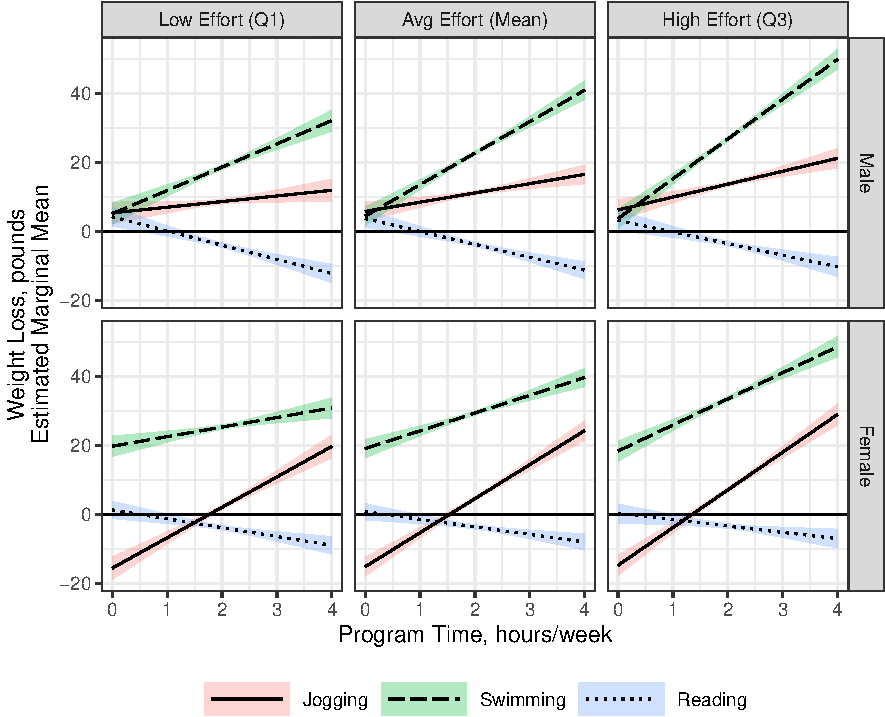
\includegraphics{Appendix_ex_weightloss_files/figure-latex/unnamed-chunk-83-1} \hfill{}

\caption{Weight Loss Uniquely Moderated by Program Time and Effort Rating According to Gender and Program Type}\label{fig:unnamed-chunk-83}
\end{figure}

\clearpage

\hypertarget{final-results}{%
\section{FINAL RESULTS}\label{final-results}}

\hypertarget{rq-1-1}{%
\subsection{RQ (1)}\label{rq-1-1}}

I'm just starting out and don't want to put in too much effort.

How many hours per week of exercise do I need to put in to lose 5
pounds?

\hypertarget{constraints}{%
\subsubsection{Constraints}\label{constraints}}

\begin{itemize}
\tightlist
\item
  Exclude the \texttt{Reading} program
\item
  Set \texttt{effort} to a low value of \texttt{26.26} out of 50 which
  is the 25th percentile (Q1)
\item
  Invert Predictions
\end{itemize}

\clearpage

\hypertarget{inverse-estimation}{%
\subsubsection{Inverse Estimation}\label{inverse-estimation}}

\begin{Shaded}
\begin{Highlighting}[]
\NormalTok{tab\_rq1 }\OtherTok{\textless{}{-}}\NormalTok{ fit\_2 }\SpecialCharTok{\%\textgreater{}\%} 
\NormalTok{  effects}\SpecialCharTok{::}\FunctionTok{Effect}\NormalTok{(}\AttributeTok{mod =}\NormalTok{ .,}
                  \AttributeTok{focal.predictors =} \FunctionTok{c}\NormalTok{(}\StringTok{"prog"}\NormalTok{, }\StringTok{"hours"}\NormalTok{, }
                                       \StringTok{"gender"}\NormalTok{, }\StringTok{"effort"}\NormalTok{),}
                  \AttributeTok{xlevels =} \FunctionTok{list}\NormalTok{(}\AttributeTok{hours =} \FunctionTok{seq}\NormalTok{(}\AttributeTok{from =} \DecValTok{0}\NormalTok{,}
                                             \AttributeTok{to =} \DecValTok{4}\NormalTok{,}
                                             \AttributeTok{by =}\NormalTok{ .}\DecValTok{1}\NormalTok{),}
                                 \AttributeTok{effort =} \FunctionTok{c}\NormalTok{(}\FloatTok{26.26}\NormalTok{, }\FloatTok{33.10}\NormalTok{))) }\SpecialCharTok{\%\textgreater{}\%} 
  \FunctionTok{data.frame}\NormalTok{() }\SpecialCharTok{\%\textgreater{}\%} 
\NormalTok{  dplyr}\SpecialCharTok{::}\FunctionTok{filter}\NormalTok{(prog }\SpecialCharTok{!=} \StringTok{"Reading"}\NormalTok{) }\SpecialCharTok{\%\textgreater{}\%} 
\NormalTok{  dplyr}\SpecialCharTok{::}\FunctionTok{filter}\NormalTok{(effort }\SpecialCharTok{==} \FloatTok{26.26}\NormalTok{) }\SpecialCharTok{\%\textgreater{}\%} 
\NormalTok{  dplyr}\SpecialCharTok{::}\FunctionTok{filter}\NormalTok{(fit }\SpecialCharTok{\textgreater{}} \DecValTok{0}\NormalTok{) }\SpecialCharTok{\%\textgreater{}\%} 
\NormalTok{  dplyr}\SpecialCharTok{::}\FunctionTok{mutate}\NormalTok{(}\AttributeTok{dist5 =} \FunctionTok{abs}\NormalTok{(fit }\SpecialCharTok{{-}} \DecValTok{5}\NormalTok{)) }\SpecialCharTok{\%\textgreater{}\%} 
\NormalTok{  dplyr}\SpecialCharTok{::}\FunctionTok{group\_by}\NormalTok{(prog, gender) }\SpecialCharTok{\%\textgreater{}\%} 
\NormalTok{  dplyr}\SpecialCharTok{::}\FunctionTok{mutate}\NormalTok{(}\AttributeTok{dist5\_min =} \FunctionTok{min}\NormalTok{(dist5)) }\SpecialCharTok{\%\textgreater{}\%} 
\NormalTok{  dplyr}\SpecialCharTok{::}\FunctionTok{filter}\NormalTok{(dist5 }\SpecialCharTok{==}\NormalTok{ dist5\_min) }\SpecialCharTok{\%\textgreater{}\%} 
\NormalTok{  dplyr}\SpecialCharTok{::}\FunctionTok{ungroup}\NormalTok{() }\SpecialCharTok{\%\textgreater{}\%} 
\NormalTok{  dplyr}\SpecialCharTok{::}\FunctionTok{arrange}\NormalTok{(prog, gender) }\SpecialCharTok{\%\textgreater{}\%} 
\NormalTok{  dplyr}\SpecialCharTok{::}\FunctionTok{select}\NormalTok{(}\StringTok{"Program"} \OtherTok{=}\NormalTok{ prog, }
                \StringTok{"Gender"} \OtherTok{=}\NormalTok{ gender, }
                \StringTok{"Exercise Time, hours/week"} \OtherTok{=}\NormalTok{ hours, }
                \StringTok{"Weight Loss, pounds"} \OtherTok{=}\NormalTok{ fit) }\SpecialCharTok{\%\textgreater{}\%} 
\NormalTok{  flextable}\SpecialCharTok{::}\FunctionTok{flextable}\NormalTok{() }\SpecialCharTok{\%\textgreater{}\%} 
\NormalTok{  flextable}\SpecialCharTok{::}\FunctionTok{set\_caption}\NormalTok{(}\AttributeTok{caption =} \StringTok{"RQ (1) Inverse Estimation of Exercise Time Required by Each Program for a Five Pound Weight Loss, Given Low Effort"}\NormalTok{)}

\NormalTok{tab\_rq1}
\end{Highlighting}
\end{Shaded}

\global\setlength{\Oldarrayrulewidth}{\arrayrulewidth}

\global\setlength{\Oldtabcolsep}{\tabcolsep}

\setlength{\tabcolsep}{2pt}

\renewcommand*{\arraystretch}{1.5}



\providecommand{\ascline}[3]{\noalign{\global\arrayrulewidth #1}\arrayrulecolor[HTML]{#2}\cline{#3}}

\begin{longtable}[l]{|p{0.75in}|p{0.75in}|p{0.75in}|p{0.75in}}

\caption{RQ\ (1)\ Inverse\ Estimation\ of\ Exercise\ Time\ Required\ by\ Each\ Program\ for\ a\ Five\ Pound\ Weight\ Loss,\ Given\ Low\ Effort}\\

\ascline{0.75pt}{000000}{1-4}

\multicolumn{1}{>{\centering}m{\dimexpr 0.75in+0\tabcolsep}}{\textcolor[HTML]{000000}{\fontsize{10}{20}\selectfont{\global\setmainfont{Times New Roman}{Program}}}} & \multicolumn{1}{>{\centering}m{\dimexpr 0.75in+0\tabcolsep}}{\textcolor[HTML]{000000}{\fontsize{10}{20}\selectfont{\global\setmainfont{Times New Roman}{Gender}}}} & \multicolumn{1}{>{\centering}m{\dimexpr 0.75in+0\tabcolsep}}{\textcolor[HTML]{000000}{\fontsize{10}{20}\selectfont{\global\setmainfont{Times New Roman}{Exercise\ Time,\ hours/week}}}} & \multicolumn{1}{>{\centering}m{\dimexpr 0.75in+0\tabcolsep}}{\textcolor[HTML]{000000}{\fontsize{10}{20}\selectfont{\global\setmainfont{Times New Roman}{Weight\ Loss,\ pounds}}}} \\

\ascline{0.75pt}{000000}{1-4}\endfirsthead \caption[]{RQ\ (1)\ Inverse\ Estimation\ of\ Exercise\ Time\ Required\ by\ Each\ Program\ for\ a\ Five\ Pound\ Weight\ Loss,\ Given\ Low\ Effort}\\

\ascline{0.75pt}{000000}{1-4}

\multicolumn{1}{>{\centering}m{\dimexpr 0.75in+0\tabcolsep}}{\textcolor[HTML]{000000}{\fontsize{10}{20}\selectfont{\global\setmainfont{Times New Roman}{Program}}}} & \multicolumn{1}{>{\centering}m{\dimexpr 0.75in+0\tabcolsep}}{\textcolor[HTML]{000000}{\fontsize{10}{20}\selectfont{\global\setmainfont{Times New Roman}{Gender}}}} & \multicolumn{1}{>{\centering}m{\dimexpr 0.75in+0\tabcolsep}}{\textcolor[HTML]{000000}{\fontsize{10}{20}\selectfont{\global\setmainfont{Times New Roman}{Exercise\ Time,\ hours/week}}}} & \multicolumn{1}{>{\centering}m{\dimexpr 0.75in+0\tabcolsep}}{\textcolor[HTML]{000000}{\fontsize{10}{20}\selectfont{\global\setmainfont{Times New Roman}{Weight\ Loss,\ pounds}}}} \\

\ascline{0.75pt}{000000}{1-4}\endhead



\multicolumn{1}{>{\centering}m{\dimexpr 0.75in+0\tabcolsep}}{\textcolor[HTML]{000000}{\fontsize{10}{20}\selectfont{\global\setmainfont{Times New Roman}{Jogging}}}} & \multicolumn{1}{>{\centering}m{\dimexpr 0.75in+0\tabcolsep}}{\textcolor[HTML]{000000}{\fontsize{10}{20}\selectfont{\global\setmainfont{Times New Roman}{Male}}}} & \multicolumn{1}{>{\centering}m{\dimexpr 0.75in+0\tabcolsep}}{\textcolor[HTML]{000000}{\fontsize{10}{20}\selectfont{\global\setmainfont{Times New Roman}{0.00}}}} & \multicolumn{1}{>{\centering}m{\dimexpr 0.75in+0\tabcolsep}}{\textcolor[HTML]{000000}{\fontsize{10}{20}\selectfont{\global\setmainfont{Times New Roman}{5.38}}}} \\





\multicolumn{1}{>{\centering}m{\dimexpr 0.75in+0\tabcolsep}}{\textcolor[HTML]{000000}{\fontsize{10}{20}\selectfont{\global\setmainfont{Times New Roman}{Jogging}}}} & \multicolumn{1}{>{\centering}m{\dimexpr 0.75in+0\tabcolsep}}{\textcolor[HTML]{000000}{\fontsize{10}{20}\selectfont{\global\setmainfont{Times New Roman}{Female}}}} & \multicolumn{1}{>{\centering}m{\dimexpr 0.75in+0\tabcolsep}}{\textcolor[HTML]{000000}{\fontsize{10}{20}\selectfont{\global\setmainfont{Times New Roman}{2.30}}}} & \multicolumn{1}{>{\centering}m{\dimexpr 0.75in+0\tabcolsep}}{\textcolor[HTML]{000000}{\fontsize{10}{20}\selectfont{\global\setmainfont{Times New Roman}{4.71}}}} \\





\multicolumn{1}{>{\centering}m{\dimexpr 0.75in+0\tabcolsep}}{\textcolor[HTML]{000000}{\fontsize{10}{20}\selectfont{\global\setmainfont{Times New Roman}{Swimming}}}} & \multicolumn{1}{>{\centering}m{\dimexpr 0.75in+0\tabcolsep}}{\textcolor[HTML]{000000}{\fontsize{10}{20}\selectfont{\global\setmainfont{Times New Roman}{Male}}}} & \multicolumn{1}{>{\centering}m{\dimexpr 0.75in+0\tabcolsep}}{\textcolor[HTML]{000000}{\fontsize{10}{20}\selectfont{\global\setmainfont{Times New Roman}{0.00}}}} & \multicolumn{1}{>{\centering}m{\dimexpr 0.75in+0\tabcolsep}}{\textcolor[HTML]{000000}{\fontsize{10}{20}\selectfont{\global\setmainfont{Times New Roman}{5.12}}}} \\





\multicolumn{1}{>{\centering}m{\dimexpr 0.75in+0\tabcolsep}}{\textcolor[HTML]{000000}{\fontsize{10}{20}\selectfont{\global\setmainfont{Times New Roman}{Swimming}}}} & \multicolumn{1}{>{\centering}m{\dimexpr 0.75in+0\tabcolsep}}{\textcolor[HTML]{000000}{\fontsize{10}{20}\selectfont{\global\setmainfont{Times New Roman}{Female}}}} & \multicolumn{1}{>{\centering}m{\dimexpr 0.75in+0\tabcolsep}}{\textcolor[HTML]{000000}{\fontsize{10}{20}\selectfont{\global\setmainfont{Times New Roman}{0.00}}}} & \multicolumn{1}{>{\centering}m{\dimexpr 0.75in+0\tabcolsep}}{\textcolor[HTML]{000000}{\fontsize{10}{20}\selectfont{\global\setmainfont{Times New Roman}{19.77}}}} \\

\ascline{0.75pt}{000000}{1-4}



\end{longtable}



\arrayrulecolor[HTML]{000000}

\global\setlength{\arrayrulewidth}{\Oldarrayrulewidth}

\global\setlength{\tabcolsep}{\Oldtabcolsep}

\renewcommand*{\arraystretch}{1}

\clearpage

\hypertarget{visualization-1}{%
\subsubsection{Visualization}\label{visualization-1}}

\begin{Shaded}
\begin{Highlighting}[]
\NormalTok{effects}\SpecialCharTok{::}\FunctionTok{Effect}\NormalTok{(}\AttributeTok{mod =}\NormalTok{ fit\_2,}
                \AttributeTok{focal.predictors =} \FunctionTok{c}\NormalTok{(}\StringTok{"prog"}\NormalTok{, }\StringTok{"hours"}\NormalTok{, }
                                     \StringTok{"gender"}\NormalTok{, }\StringTok{"effort"}\NormalTok{),}
                \AttributeTok{xlevels =} \FunctionTok{list}\NormalTok{(}\AttributeTok{hours =} \FunctionTok{seq}\NormalTok{(}\AttributeTok{from =} \DecValTok{0}\NormalTok{,}
                                           \AttributeTok{to =} \DecValTok{4}\NormalTok{,}
                                           \AttributeTok{by =}\NormalTok{ .}\DecValTok{1}\NormalTok{),}
                               \AttributeTok{effort =} \FunctionTok{c}\NormalTok{(}\FloatTok{26.26}\NormalTok{, }\FloatTok{29.66}\NormalTok{, }\FloatTok{33.10}\NormalTok{))) }\SpecialCharTok{\%\textgreater{}\%} 
  \FunctionTok{data.frame}\NormalTok{() }\SpecialCharTok{\%\textgreater{}\%} 
\NormalTok{  dplyr}\SpecialCharTok{::}\FunctionTok{filter}\NormalTok{(prog }\SpecialCharTok{!=} \StringTok{"Reading"}\NormalTok{) }\SpecialCharTok{\%\textgreater{}\%} 
\NormalTok{  dplyr}\SpecialCharTok{::}\FunctionTok{filter}\NormalTok{(effort }\SpecialCharTok{==} \FloatTok{26.26}\NormalTok{) }\SpecialCharTok{\%\textgreater{}\%} 
  \FunctionTok{ggplot}\NormalTok{(}\FunctionTok{aes}\NormalTok{(}\AttributeTok{x =}\NormalTok{ hours,}
             \AttributeTok{y =}\NormalTok{ fit,}
             \AttributeTok{group =}\NormalTok{ prog)) }\SpecialCharTok{+}
  \FunctionTok{geom\_ribbon}\NormalTok{(}\FunctionTok{aes}\NormalTok{(}\AttributeTok{ymin =}\NormalTok{ lower,}
                  \AttributeTok{ymax =}\NormalTok{ upper,}
                  \AttributeTok{fill =}\NormalTok{ prog),}
              \AttributeTok{alpha =}\NormalTok{ .}\DecValTok{3}\NormalTok{) }\SpecialCharTok{+}
  \FunctionTok{geom\_line}\NormalTok{(}\FunctionTok{aes}\NormalTok{(}\AttributeTok{linetype =}\NormalTok{ prog)) }\SpecialCharTok{+}
  \FunctionTok{theme\_bw}\NormalTok{() }\SpecialCharTok{+}
  \FunctionTok{facet\_grid}\NormalTok{(}\SpecialCharTok{\textasciitilde{}}\NormalTok{ gender) }\SpecialCharTok{+}
  \FunctionTok{geom\_hline}\NormalTok{(}\AttributeTok{yintercept =} \DecValTok{0}\NormalTok{,}
             \AttributeTok{color =} \StringTok{"blaCK"}\NormalTok{)}\SpecialCharTok{+}
  \FunctionTok{geom\_hline}\NormalTok{(}\AttributeTok{yintercept =} \DecValTok{5}\NormalTok{,}
             \AttributeTok{color =} \StringTok{"red"}\NormalTok{)}\SpecialCharTok{+}
  \FunctionTok{scale\_linetype\_manual}\NormalTok{(}\AttributeTok{values =} \FunctionTok{c}\NormalTok{(}\StringTok{"solid"}\NormalTok{, }\StringTok{"longdash"}\NormalTok{, }\StringTok{"dotted"}\NormalTok{)) }\SpecialCharTok{+}
  \FunctionTok{scale\_fill\_manual}\NormalTok{(}\AttributeTok{values =} \FunctionTok{c}\NormalTok{(}\StringTok{"gray20"}\NormalTok{, }\StringTok{"gray90"}\NormalTok{)) }\SpecialCharTok{+}
  \FunctionTok{scale\_y\_continuous}\NormalTok{(}\AttributeTok{breaks =} \FunctionTok{seq}\NormalTok{(}\AttributeTok{from =} \SpecialCharTok{{-}}\DecValTok{20}\NormalTok{, }\AttributeTok{to =} \DecValTok{50}\NormalTok{, }\AttributeTok{by =} \DecValTok{10}\NormalTok{)) }\SpecialCharTok{+}
  \FunctionTok{labs}\NormalTok{(}\AttributeTok{x =} \StringTok{"Program Time, hours/week"}\NormalTok{,}
       \AttributeTok{y =} \StringTok{"Weight Loss, pounds}\SpecialCharTok{\textbackslash{}n}\StringTok{Estimated Marginal Mean"}\NormalTok{,}
       \AttributeTok{linetype =} \ConstantTok{NULL}\NormalTok{,}
       \AttributeTok{fill =} \ConstantTok{NULL}\NormalTok{)  }\SpecialCharTok{+}
  \FunctionTok{theme}\NormalTok{(}\AttributeTok{legend.position =} \FunctionTok{c}\NormalTok{(}\DecValTok{1}\NormalTok{, }\DecValTok{0}\NormalTok{),}
        \AttributeTok{legend.justification =} \FunctionTok{c}\NormalTok{(}\FloatTok{1.1}\NormalTok{, }\SpecialCharTok{{-}}\NormalTok{.}\DecValTok{1}\NormalTok{),}
        \AttributeTok{legend.background =} \FunctionTok{element\_rect}\NormalTok{(}\AttributeTok{color =} \StringTok{"black"}\NormalTok{),}
        \AttributeTok{legend.key.width =} \FunctionTok{unit}\NormalTok{(}\FloatTok{1.5}\NormalTok{, }\StringTok{"cm"}\NormalTok{)) }\SpecialCharTok{+}
  \FunctionTok{geom\_point}\NormalTok{(}\AttributeTok{data =} \FunctionTok{data.frame}\NormalTok{(}\AttributeTok{gender =} \StringTok{"Female"}\NormalTok{,}
                               \AttributeTok{prog =} \StringTok{"Jogging"}\NormalTok{,}
                               \AttributeTok{hours =} \FloatTok{2.3}\NormalTok{,}
                               \AttributeTok{fit =} \DecValTok{5}\NormalTok{),}
             \AttributeTok{color =} \StringTok{"red"}\NormalTok{,}
             \AttributeTok{shape =} \DecValTok{1}\NormalTok{,}
             \AttributeTok{size =} \DecValTok{5}\NormalTok{) }
\end{Highlighting}
\end{Shaded}

\begin{figure}[hb]

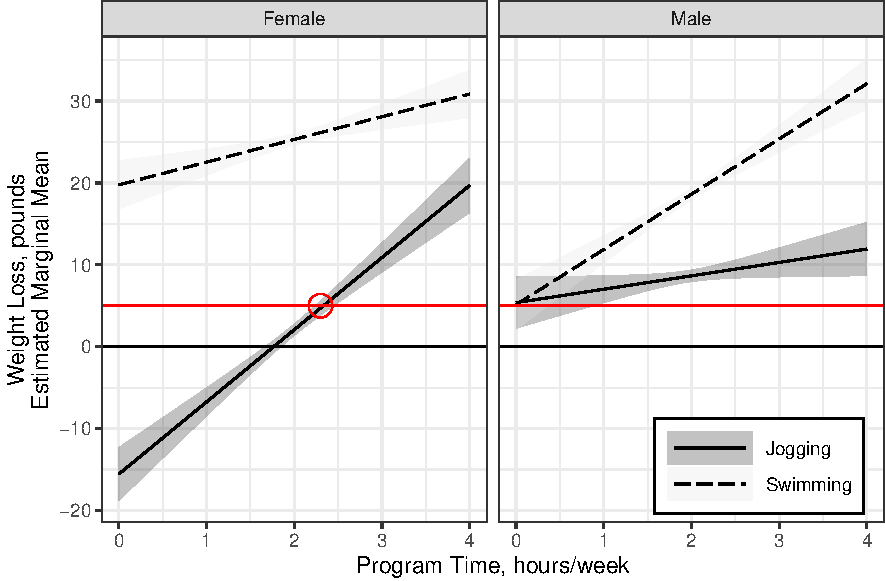
\includegraphics{Appendix_ex_weightloss_files/figure-latex/unnamed-chunk-87-1} \hfill{}

\caption{RQ (1) Compare Exercise Time Required by Each Program for a Five Pound Weight Loss, Given Low Effort}\label{fig:unnamed-chunk-87}
\end{figure}

\clearpage

\hypertarget{conclusion}{%
\subsubsection{Conclusion}\label{conclusion}}

\begin{itemize}
\item
  Even when putting in little effort, both men and women on the swimming
  program should expect at least a 5 pound weight loss, irrespective of
  weekly time spent.
\item
  While men should also expect a 5+ pound weight loss on the jogging
  program, irrespective of weekly time spent, women will need to plan on
  spending at least 2 hours and 20 min per week running.
\end{itemize}

\clearpage

\hypertarget{rq-2-1}{%
\subsection{RQ (2)}\label{rq-2-1}}

I'm moderately fit and can put in an average level of effort into my
workout.

For every one hour increase per week in exercise, how much additional
weight loss do I expect?

\hypertarget{constraints-1}{%
\subsubsection{Constraints}\label{constraints-1}}

\begin{itemize}
\tightlist
\item
  Exclude the \texttt{Reading} program
\item
  Set \texttt{effort} to the mean value
\item
  Interpret the slopes, \texttt{b}
\end{itemize}

\hypertarget{simple-slopes-analysis-1}{%
\subsubsection{Simple Slopes Analysis}\label{simple-slopes-analysis-1}}

\begin{Shaded}
\begin{Highlighting}[]
\NormalTok{sim\_slope\_M }\OtherTok{\textless{}{-}}\NormalTok{ fit\_2 }\SpecialCharTok{\%\textgreater{}\%} 
\NormalTok{  emmeans}\SpecialCharTok{::}\FunctionTok{emtrends}\NormalTok{(}\AttributeTok{var =} \StringTok{"hours"}\NormalTok{, }
                    \SpecialCharTok{\textasciitilde{}}\NormalTok{ prog }\SpecialCharTok{|}\NormalTok{ gender) }\SpecialCharTok{\%\textgreater{}\%} 
  \FunctionTok{data.frame}\NormalTok{() }\SpecialCharTok{\%\textgreater{}\%} 
\NormalTok{  dplyr}\SpecialCharTok{::}\FunctionTok{filter}\NormalTok{(prog }\SpecialCharTok{!=} \StringTok{"Reading"}\NormalTok{) }
\end{Highlighting}
\end{Shaded}

\begin{Shaded}
\begin{Highlighting}[]
\NormalTok{tab\_rq2 }\OtherTok{\textless{}{-}}\NormalTok{ sim\_slope\_M }\SpecialCharTok{\%\textgreater{}\%} 
\NormalTok{  dplyr}\SpecialCharTok{::}\FunctionTok{select}\NormalTok{(}\AttributeTok{Program =}\NormalTok{ prog,}
                \AttributeTok{Gender =}\NormalTok{ gender,}
                \AttributeTok{Slope =}\NormalTok{ hours.trend,}
\NormalTok{                SE, lower.CL, upper.CL) }\SpecialCharTok{\%\textgreater{}\%} 
\NormalTok{  dplyr}\SpecialCharTok{::}\FunctionTok{mutate\_if}\NormalTok{(is.numeric, apaSupp}\SpecialCharTok{::}\NormalTok{apa2) }\SpecialCharTok{\%\textgreater{}\%} 
\NormalTok{  flextable}\SpecialCharTok{::}\FunctionTok{flextable}\NormalTok{()}\SpecialCharTok{\%\textgreater{}\%} 
\NormalTok{  flextable}\SpecialCharTok{::}\FunctionTok{set\_caption}\NormalTok{(}\StringTok{"RQ (2) Additional Weight Loss per Hour/Week Spent on Each Exercise Program with Average Effort, by Gender"}\NormalTok{)}

\NormalTok{tab\_rq2}
\end{Highlighting}
\end{Shaded}

\global\setlength{\Oldarrayrulewidth}{\arrayrulewidth}

\global\setlength{\Oldtabcolsep}{\tabcolsep}

\setlength{\tabcolsep}{2pt}

\renewcommand*{\arraystretch}{1.5}



\providecommand{\ascline}[3]{\noalign{\global\arrayrulewidth #1}\arrayrulecolor[HTML]{#2}\cline{#3}}

\begin{longtable}[l]{|p{0.75in}|p{0.75in}|p{0.75in}|p{0.75in}|p{0.75in}|p{0.75in}}

\caption{RQ\ (2)\ Additional\ Weight\ Loss\ per\ Hour/Week\ Spent\ on\ Each\ Exercise\ Program\ with\ Average\ Effort,\ by\ Gender}\\

\ascline{0.75pt}{000000}{1-6}

\multicolumn{1}{>{\centering}m{\dimexpr 0.75in+0\tabcolsep}}{\textcolor[HTML]{000000}{\fontsize{10}{20}\selectfont{\global\setmainfont{Times New Roman}{Program}}}} & \multicolumn{1}{>{\centering}m{\dimexpr 0.75in+0\tabcolsep}}{\textcolor[HTML]{000000}{\fontsize{10}{20}\selectfont{\global\setmainfont{Times New Roman}{Gender}}}} & \multicolumn{1}{>{\centering}m{\dimexpr 0.75in+0\tabcolsep}}{\textcolor[HTML]{000000}{\fontsize{10}{20}\selectfont{\global\setmainfont{Times New Roman}{Slope}}}} & \multicolumn{1}{>{\centering}m{\dimexpr 0.75in+0\tabcolsep}}{\textcolor[HTML]{000000}{\fontsize{10}{20}\selectfont{\global\setmainfont{Times New Roman}{SE}}}} & \multicolumn{1}{>{\centering}m{\dimexpr 0.75in+0\tabcolsep}}{\textcolor[HTML]{000000}{\fontsize{10}{20}\selectfont{\global\setmainfont{Times New Roman}{lower.CL}}}} & \multicolumn{1}{>{\centering}m{\dimexpr 0.75in+0\tabcolsep}}{\textcolor[HTML]{000000}{\fontsize{10}{20}\selectfont{\global\setmainfont{Times New Roman}{upper.CL}}}} \\

\ascline{0.75pt}{000000}{1-6}\endfirsthead \caption[]{RQ\ (2)\ Additional\ Weight\ Loss\ per\ Hour/Week\ Spent\ on\ Each\ Exercise\ Program\ with\ Average\ Effort,\ by\ Gender}\\

\ascline{0.75pt}{000000}{1-6}

\multicolumn{1}{>{\centering}m{\dimexpr 0.75in+0\tabcolsep}}{\textcolor[HTML]{000000}{\fontsize{10}{20}\selectfont{\global\setmainfont{Times New Roman}{Program}}}} & \multicolumn{1}{>{\centering}m{\dimexpr 0.75in+0\tabcolsep}}{\textcolor[HTML]{000000}{\fontsize{10}{20}\selectfont{\global\setmainfont{Times New Roman}{Gender}}}} & \multicolumn{1}{>{\centering}m{\dimexpr 0.75in+0\tabcolsep}}{\textcolor[HTML]{000000}{\fontsize{10}{20}\selectfont{\global\setmainfont{Times New Roman}{Slope}}}} & \multicolumn{1}{>{\centering}m{\dimexpr 0.75in+0\tabcolsep}}{\textcolor[HTML]{000000}{\fontsize{10}{20}\selectfont{\global\setmainfont{Times New Roman}{SE}}}} & \multicolumn{1}{>{\centering}m{\dimexpr 0.75in+0\tabcolsep}}{\textcolor[HTML]{000000}{\fontsize{10}{20}\selectfont{\global\setmainfont{Times New Roman}{lower.CL}}}} & \multicolumn{1}{>{\centering}m{\dimexpr 0.75in+0\tabcolsep}}{\textcolor[HTML]{000000}{\fontsize{10}{20}\selectfont{\global\setmainfont{Times New Roman}{upper.CL}}}} \\

\ascline{0.75pt}{000000}{1-6}\endhead



\multicolumn{1}{>{\centering}m{\dimexpr 0.75in+0\tabcolsep}}{\textcolor[HTML]{000000}{\fontsize{10}{20}\selectfont{\global\setmainfont{Times New Roman}{Jogging}}}} & \multicolumn{1}{>{\centering}m{\dimexpr 0.75in+0\tabcolsep}}{\textcolor[HTML]{000000}{\fontsize{10}{20}\selectfont{\global\setmainfont{Times New Roman}{Male}}}} & \multicolumn{1}{>{\centering}m{\dimexpr 0.75in+0\tabcolsep}}{\textcolor[HTML]{000000}{\fontsize{10}{20}\selectfont{\global\setmainfont{Times New Roman}{2.68}}}} & \multicolumn{1}{>{\centering}m{\dimexpr 0.75in+0\tabcolsep}}{\textcolor[HTML]{000000}{\fontsize{10}{20}\selectfont{\global\setmainfont{Times New Roman}{0.67}}}} & \multicolumn{1}{>{\centering}m{\dimexpr 0.75in+0\tabcolsep}}{\textcolor[HTML]{000000}{\fontsize{10}{20}\selectfont{\global\setmainfont{Times New Roman}{1.36}}}} & \multicolumn{1}{>{\centering}m{\dimexpr 0.75in+0\tabcolsep}}{\textcolor[HTML]{000000}{\fontsize{10}{20}\selectfont{\global\setmainfont{Times New Roman}{\ 4.01}}}} \\





\multicolumn{1}{>{\centering}m{\dimexpr 0.75in+0\tabcolsep}}{\textcolor[HTML]{000000}{\fontsize{10}{20}\selectfont{\global\setmainfont{Times New Roman}{Swimming}}}} & \multicolumn{1}{>{\centering}m{\dimexpr 0.75in+0\tabcolsep}}{\textcolor[HTML]{000000}{\fontsize{10}{20}\selectfont{\global\setmainfont{Times New Roman}{Male}}}} & \multicolumn{1}{>{\centering}m{\dimexpr 0.75in+0\tabcolsep}}{\textcolor[HTML]{000000}{\fontsize{10}{20}\selectfont{\global\setmainfont{Times New Roman}{9.13}}}} & \multicolumn{1}{>{\centering}m{\dimexpr 0.75in+0\tabcolsep}}{\textcolor[HTML]{000000}{\fontsize{10}{20}\selectfont{\global\setmainfont{Times New Roman}{0.66}}}} & \multicolumn{1}{>{\centering}m{\dimexpr 0.75in+0\tabcolsep}}{\textcolor[HTML]{000000}{\fontsize{10}{20}\selectfont{\global\setmainfont{Times New Roman}{7.84}}}} & \multicolumn{1}{>{\centering}m{\dimexpr 0.75in+0\tabcolsep}}{\textcolor[HTML]{000000}{\fontsize{10}{20}\selectfont{\global\setmainfont{Times New Roman}{10.41}}}} \\





\multicolumn{1}{>{\centering}m{\dimexpr 0.75in+0\tabcolsep}}{\textcolor[HTML]{000000}{\fontsize{10}{20}\selectfont{\global\setmainfont{Times New Roman}{Jogging}}}} & \multicolumn{1}{>{\centering}m{\dimexpr 0.75in+0\tabcolsep}}{\textcolor[HTML]{000000}{\fontsize{10}{20}\selectfont{\global\setmainfont{Times New Roman}{Female}}}} & \multicolumn{1}{>{\centering}m{\dimexpr 0.75in+0\tabcolsep}}{\textcolor[HTML]{000000}{\fontsize{10}{20}\selectfont{\global\setmainfont{Times New Roman}{9.86}}}} & \multicolumn{1}{>{\centering}m{\dimexpr 0.75in+0\tabcolsep}}{\textcolor[HTML]{000000}{\fontsize{10}{20}\selectfont{\global\setmainfont{Times New Roman}{0.70}}}} & \multicolumn{1}{>{\centering}m{\dimexpr 0.75in+0\tabcolsep}}{\textcolor[HTML]{000000}{\fontsize{10}{20}\selectfont{\global\setmainfont{Times New Roman}{8.49}}}} & \multicolumn{1}{>{\centering}m{\dimexpr 0.75in+0\tabcolsep}}{\textcolor[HTML]{000000}{\fontsize{10}{20}\selectfont{\global\setmainfont{Times New Roman}{11.24}}}} \\





\multicolumn{1}{>{\centering}m{\dimexpr 0.75in+0\tabcolsep}}{\textcolor[HTML]{000000}{\fontsize{10}{20}\selectfont{\global\setmainfont{Times New Roman}{Swimming}}}} & \multicolumn{1}{>{\centering}m{\dimexpr 0.75in+0\tabcolsep}}{\textcolor[HTML]{000000}{\fontsize{10}{20}\selectfont{\global\setmainfont{Times New Roman}{Female}}}} & \multicolumn{1}{>{\centering}m{\dimexpr 0.75in+0\tabcolsep}}{\textcolor[HTML]{000000}{\fontsize{10}{20}\selectfont{\global\setmainfont{Times New Roman}{5.15}}}} & \multicolumn{1}{>{\centering}m{\dimexpr 0.75in+0\tabcolsep}}{\textcolor[HTML]{000000}{\fontsize{10}{20}\selectfont{\global\setmainfont{Times New Roman}{0.66}}}} & \multicolumn{1}{>{\centering}m{\dimexpr 0.75in+0\tabcolsep}}{\textcolor[HTML]{000000}{\fontsize{10}{20}\selectfont{\global\setmainfont{Times New Roman}{3.86}}}} & \multicolumn{1}{>{\centering}m{\dimexpr 0.75in+0\tabcolsep}}{\textcolor[HTML]{000000}{\fontsize{10}{20}\selectfont{\global\setmainfont{Times New Roman}{\ 6.44}}}} \\

\ascline{0.75pt}{000000}{1-6}



\end{longtable}



\arrayrulecolor[HTML]{000000}

\global\setlength{\arrayrulewidth}{\Oldarrayrulewidth}

\global\setlength{\tabcolsep}{\Oldtabcolsep}

\renewcommand*{\arraystretch}{1}

\clearpage

\hypertarget{visualize}{%
\subsubsection{Visualize}\label{visualize}}

\begin{Shaded}
\begin{Highlighting}[]
\NormalTok{effects}\SpecialCharTok{::}\FunctionTok{Effect}\NormalTok{(}\AttributeTok{mod =}\NormalTok{ fit\_2,}
                \AttributeTok{focal.predictors =} \FunctionTok{c}\NormalTok{(}\StringTok{"prog"}\NormalTok{, }\StringTok{"hours"}\NormalTok{, }
                                     \StringTok{"gender"}\NormalTok{, }\StringTok{"effort"}\NormalTok{),}
                \AttributeTok{xlevels =} \FunctionTok{list}\NormalTok{(}\AttributeTok{hours =} \FunctionTok{seq}\NormalTok{(}\AttributeTok{from =} \DecValTok{0}\NormalTok{,}
                                           \AttributeTok{to =} \DecValTok{4}\NormalTok{,}
                                           \AttributeTok{by =}\NormalTok{ .}\DecValTok{1}\NormalTok{),}
                               \AttributeTok{effort =} \FunctionTok{c}\NormalTok{( }\FloatTok{26.26}\NormalTok{, }\FloatTok{29.63}\NormalTok{, }\FloatTok{33.10}\NormalTok{))) }\SpecialCharTok{\%\textgreater{}\%} 
  \FunctionTok{data.frame}\NormalTok{() }\SpecialCharTok{\%\textgreater{}\%} 
\NormalTok{  dplyr}\SpecialCharTok{::}\FunctionTok{filter}\NormalTok{(prog }\SpecialCharTok{!=} \StringTok{"Reading"}\NormalTok{) }\SpecialCharTok{\%\textgreater{}\%} 
\NormalTok{  dplyr}\SpecialCharTok{::}\FunctionTok{filter}\NormalTok{(effort }\SpecialCharTok{==} \FloatTok{33.10}\NormalTok{) }\SpecialCharTok{\%\textgreater{}\%} 
  \FunctionTok{ggplot}\NormalTok{(}\FunctionTok{aes}\NormalTok{(}\AttributeTok{x =}\NormalTok{ hours,}
             \AttributeTok{y =}\NormalTok{ fit,}
             \AttributeTok{group =}\NormalTok{ prog)) }\SpecialCharTok{+}
  \FunctionTok{geom\_ribbon}\NormalTok{(}\FunctionTok{aes}\NormalTok{(}\AttributeTok{ymin =}\NormalTok{ lower,}
                  \AttributeTok{ymax =}\NormalTok{ upper,}
                  \AttributeTok{fill =}\NormalTok{ prog),}
              \AttributeTok{alpha =}\NormalTok{ .}\DecValTok{3}\NormalTok{) }\SpecialCharTok{+}
  \FunctionTok{geom\_line}\NormalTok{(}\FunctionTok{aes}\NormalTok{(}\AttributeTok{linetype =}\NormalTok{ prog)) }\SpecialCharTok{+}
  \FunctionTok{theme\_bw}\NormalTok{() }\SpecialCharTok{+}
  \FunctionTok{facet\_grid}\NormalTok{(}\SpecialCharTok{\textasciitilde{}}\NormalTok{ gender) }\SpecialCharTok{+}
  \FunctionTok{geom\_hline}\NormalTok{(}\AttributeTok{yintercept =} \DecValTok{0}\NormalTok{,}
             \AttributeTok{color =} \StringTok{"blaCK"}\NormalTok{)}\SpecialCharTok{+}
  \FunctionTok{scale\_linetype\_manual}\NormalTok{(}\AttributeTok{values =} \FunctionTok{c}\NormalTok{(}\StringTok{"solid"}\NormalTok{, }\StringTok{"longdash"}\NormalTok{, }\StringTok{"dotted"}\NormalTok{)) }\SpecialCharTok{+}
  \FunctionTok{scale\_y\_continuous}\NormalTok{(}\AttributeTok{breaks =} \FunctionTok{seq}\NormalTok{(}\AttributeTok{from =} \SpecialCharTok{{-}}\DecValTok{20}\NormalTok{, }\AttributeTok{to =} \DecValTok{50}\NormalTok{, }\AttributeTok{by =} \DecValTok{10}\NormalTok{)) }\SpecialCharTok{+}
  \FunctionTok{scale\_fill\_manual}\NormalTok{(}\AttributeTok{values =} \FunctionTok{c}\NormalTok{(}\StringTok{"gray20"}\NormalTok{, }\StringTok{"gray90"}\NormalTok{)) }\SpecialCharTok{+}
  \FunctionTok{labs}\NormalTok{(}\AttributeTok{x =} \StringTok{"Program Time, hours/week"}\NormalTok{,}
       \AttributeTok{y =} \StringTok{"Weight Loss, pounds}\SpecialCharTok{\textbackslash{}n}\StringTok{Estimated Marginal Mean"}\NormalTok{,}
       \AttributeTok{linetype =} \ConstantTok{NULL}\NormalTok{,}
       \AttributeTok{fill =} \ConstantTok{NULL}\NormalTok{)  }\SpecialCharTok{+}
  \FunctionTok{theme}\NormalTok{(}\AttributeTok{legend.position =} \FunctionTok{c}\NormalTok{(}\DecValTok{0}\NormalTok{, }\DecValTok{1}\NormalTok{),}
        \AttributeTok{legend.justification =} \FunctionTok{c}\NormalTok{(}\SpecialCharTok{{-}}\NormalTok{.}\DecValTok{1}\NormalTok{, }\FloatTok{1.1}\NormalTok{),}
        \AttributeTok{legend.background =} \FunctionTok{element\_rect}\NormalTok{(}\AttributeTok{color =} \StringTok{"black"}\NormalTok{)) }\SpecialCharTok{+}
  \FunctionTok{geom\_text}\NormalTok{(}\AttributeTok{data =}\NormalTok{ sim\_slope\_M }\SpecialCharTok{\%\textgreater{}\%} 
\NormalTok{              dplyr}\SpecialCharTok{::}\FunctionTok{mutate}\NormalTok{(}\AttributeTok{hours =} \FunctionTok{c}\NormalTok{(}\DecValTok{3}\NormalTok{, .}\DecValTok{75}\NormalTok{, }\DecValTok{3}\NormalTok{, }\FloatTok{0.9}\NormalTok{),}
                            \AttributeTok{fit =} \FunctionTok{c}\NormalTok{(}\DecValTok{13}\NormalTok{, }\DecValTok{18}\NormalTok{, }\DecValTok{13}\NormalTok{, }\DecValTok{30}\NormalTok{)),}
            \FunctionTok{aes}\NormalTok{(}\AttributeTok{label =}\NormalTok{ glue}\SpecialCharTok{::}\FunctionTok{glue}\NormalTok{(}\StringTok{"\{apaSupp::apa2(hours.trend)\}"}\NormalTok{)))}
\end{Highlighting}
\end{Shaded}

\begin{figure}[hb]

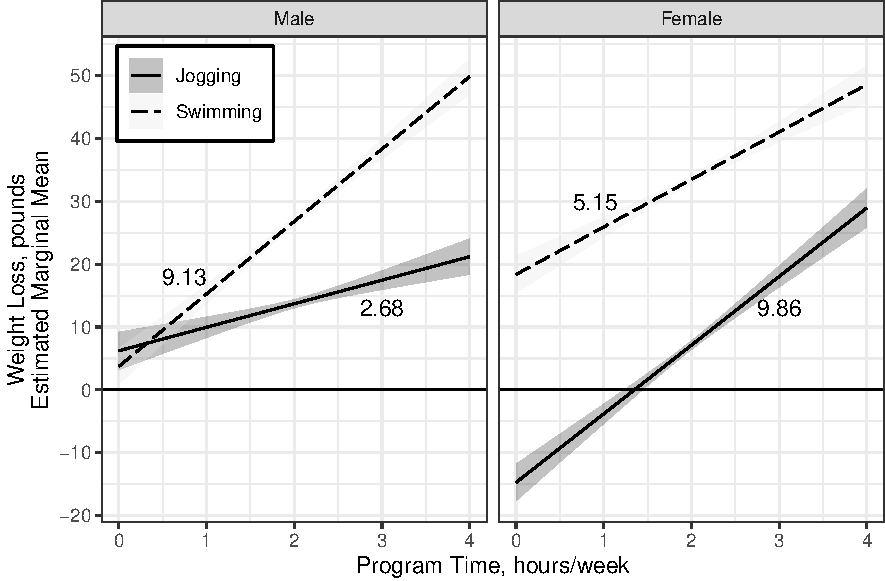
\includegraphics{Appendix_ex_weightloss_files/figure-latex/unnamed-chunk-92-1} \hfill{}

\caption{RQ (2) Compare Additional Weight Loss per Hour/Week Spent on Each Exercise Program with Average Effort, by Gender}\label{fig:unnamed-chunk-92}
\end{figure}

\clearpage

\hypertarget{conclusion-1}{%
\subsubsection{Conclusion}\label{conclusion-1}}

An hour increase per week in exercise, will result in a different amount
of additional total weight loss, depending on gender and program type.

For women, an hour/week increase in exercise will translate to 9.86 more
pounds loss if jogging and 5.15 if swimming.

For men, an hour/week increase in exercise will translate to 2.68 more
pounds loss if jogging and 9.13 if swimming.

\clearpage

\hypertarget{rq-3-1}{%
\subsection{RQ (3)}\label{rq-3-1}}

I'm a crossfit athlete and can perform with the utmost intensity.

How much more weight loss would I expect for every one hour increase in
exercise compared to the average amount of effort most people put in?

Additionally, we can visualize the interaction to help us understand
these relationships.

\hypertarget{contraints}{%
\subsubsection{Contraints}\label{contraints}}

\begin{itemize}
\tightlist
\item
  Exclude the \texttt{Reading} program
\item
  Set \texttt{effort} to near the max: 45
\item
  Interpret the slopes, \texttt{b}
\end{itemize}

\clearpage

\hypertarget{simple-slopes-analysis-2}{%
\subsubsection{Simple Slopes Analysis}\label{simple-slopes-analysis-2}}

\begin{Shaded}
\begin{Highlighting}[]
\NormalTok{sim\_slope\_Max }\OtherTok{\textless{}{-}}\NormalTok{ fit\_2 }\SpecialCharTok{\%\textgreater{}\%} 
\NormalTok{  emmeans}\SpecialCharTok{::}\FunctionTok{emtrends}\NormalTok{(}\AttributeTok{var =} \StringTok{"hours"}\NormalTok{, }
                    \SpecialCharTok{\textasciitilde{}}\NormalTok{ prog }\SpecialCharTok{|}\NormalTok{ gender,}
                    \AttributeTok{at =} \FunctionTok{list}\NormalTok{(}\AttributeTok{effort =} \DecValTok{45}\NormalTok{)) }\SpecialCharTok{\%\textgreater{}\%} 
  \FunctionTok{data.frame}\NormalTok{() }\SpecialCharTok{\%\textgreater{}\%} 
\NormalTok{  dplyr}\SpecialCharTok{::}\FunctionTok{filter}\NormalTok{(prog }\SpecialCharTok{!=} \StringTok{"Reading"}\NormalTok{) }
\end{Highlighting}
\end{Shaded}

\begin{Shaded}
\begin{Highlighting}[]
\NormalTok{tab\_rq3a }\OtherTok{\textless{}{-}}\NormalTok{ sim\_slope\_Max }\SpecialCharTok{\%\textgreater{}\%} 
\NormalTok{  dplyr}\SpecialCharTok{::}\FunctionTok{select}\NormalTok{(}\AttributeTok{Program =}\NormalTok{ prog,}
                \AttributeTok{Gender =}\NormalTok{ gender,}
                \AttributeTok{Slope =}\NormalTok{ hours.trend,}
\NormalTok{                SE, lower.CL, upper.CL) }\SpecialCharTok{\%\textgreater{}\%} 
\NormalTok{  dplyr}\SpecialCharTok{::}\FunctionTok{mutate\_if}\NormalTok{(is.numeric, apaSupp}\SpecialCharTok{::}\NormalTok{apa2) }\SpecialCharTok{\%\textgreater{}\%} 
\NormalTok{  flextable}\SpecialCharTok{::}\FunctionTok{flextable}\NormalTok{()}\SpecialCharTok{\%\textgreater{}\%} 
\NormalTok{  flextable}\SpecialCharTok{::}\FunctionTok{set\_caption}\NormalTok{(}\StringTok{"RQ (3) Additional Weight Loss per Hour/Week Spent on Each Exercise Program with Near Maximum Effort, by Gender"}\NormalTok{)}

\NormalTok{tab\_rq3a}
\end{Highlighting}
\end{Shaded}

\global\setlength{\Oldarrayrulewidth}{\arrayrulewidth}

\global\setlength{\Oldtabcolsep}{\tabcolsep}

\setlength{\tabcolsep}{2pt}

\renewcommand*{\arraystretch}{1.5}



\providecommand{\ascline}[3]{\noalign{\global\arrayrulewidth #1}\arrayrulecolor[HTML]{#2}\cline{#3}}

\begin{longtable}[l]{|p{0.75in}|p{0.75in}|p{0.75in}|p{0.75in}|p{0.75in}|p{0.75in}}

\caption{RQ\ (3)\ Additional\ Weight\ Loss\ per\ Hour/Week\ Spent\ on\ Each\ Exercise\ Program\ with\ Near\ Maximum\ Effort,\ by\ Gender}\\

\ascline{0.75pt}{000000}{1-6}

\multicolumn{1}{>{\centering}m{\dimexpr 0.75in+0\tabcolsep}}{\textcolor[HTML]{000000}{\fontsize{10}{20}\selectfont{\global\setmainfont{Times New Roman}{Program}}}} & \multicolumn{1}{>{\centering}m{\dimexpr 0.75in+0\tabcolsep}}{\textcolor[HTML]{000000}{\fontsize{10}{20}\selectfont{\global\setmainfont{Times New Roman}{Gender}}}} & \multicolumn{1}{>{\centering}m{\dimexpr 0.75in+0\tabcolsep}}{\textcolor[HTML]{000000}{\fontsize{10}{20}\selectfont{\global\setmainfont{Times New Roman}{Slope}}}} & \multicolumn{1}{>{\centering}m{\dimexpr 0.75in+0\tabcolsep}}{\textcolor[HTML]{000000}{\fontsize{10}{20}\selectfont{\global\setmainfont{Times New Roman}{SE}}}} & \multicolumn{1}{>{\centering}m{\dimexpr 0.75in+0\tabcolsep}}{\textcolor[HTML]{000000}{\fontsize{10}{20}\selectfont{\global\setmainfont{Times New Roman}{lower.CL}}}} & \multicolumn{1}{>{\centering}m{\dimexpr 0.75in+0\tabcolsep}}{\textcolor[HTML]{000000}{\fontsize{10}{20}\selectfont{\global\setmainfont{Times New Roman}{upper.CL}}}} \\

\ascline{0.75pt}{000000}{1-6}\endfirsthead \caption[]{RQ\ (3)\ Additional\ Weight\ Loss\ per\ Hour/Week\ Spent\ on\ Each\ Exercise\ Program\ with\ Near\ Maximum\ Effort,\ by\ Gender}\\

\ascline{0.75pt}{000000}{1-6}

\multicolumn{1}{>{\centering}m{\dimexpr 0.75in+0\tabcolsep}}{\textcolor[HTML]{000000}{\fontsize{10}{20}\selectfont{\global\setmainfont{Times New Roman}{Program}}}} & \multicolumn{1}{>{\centering}m{\dimexpr 0.75in+0\tabcolsep}}{\textcolor[HTML]{000000}{\fontsize{10}{20}\selectfont{\global\setmainfont{Times New Roman}{Gender}}}} & \multicolumn{1}{>{\centering}m{\dimexpr 0.75in+0\tabcolsep}}{\textcolor[HTML]{000000}{\fontsize{10}{20}\selectfont{\global\setmainfont{Times New Roman}{Slope}}}} & \multicolumn{1}{>{\centering}m{\dimexpr 0.75in+0\tabcolsep}}{\textcolor[HTML]{000000}{\fontsize{10}{20}\selectfont{\global\setmainfont{Times New Roman}{SE}}}} & \multicolumn{1}{>{\centering}m{\dimexpr 0.75in+0\tabcolsep}}{\textcolor[HTML]{000000}{\fontsize{10}{20}\selectfont{\global\setmainfont{Times New Roman}{lower.CL}}}} & \multicolumn{1}{>{\centering}m{\dimexpr 0.75in+0\tabcolsep}}{\textcolor[HTML]{000000}{\fontsize{10}{20}\selectfont{\global\setmainfont{Times New Roman}{upper.CL}}}} \\

\ascline{0.75pt}{000000}{1-6}\endhead



\multicolumn{1}{>{\centering}m{\dimexpr 0.75in+0\tabcolsep}}{\textcolor[HTML]{000000}{\fontsize{10}{20}\selectfont{\global\setmainfont{Times New Roman}{Jogging}}}} & \multicolumn{1}{>{\centering}m{\dimexpr 0.75in+0\tabcolsep}}{\textcolor[HTML]{000000}{\fontsize{10}{20}\selectfont{\global\setmainfont{Times New Roman}{Male}}}} & \multicolumn{1}{>{\centering}m{\dimexpr 0.75in+0\tabcolsep}}{\textcolor[HTML]{000000}{\fontsize{10}{20}\selectfont{\global\setmainfont{Times New Roman}{\ 7.41}}}} & \multicolumn{1}{>{\centering}m{\dimexpr 0.75in+0\tabcolsep}}{\textcolor[HTML]{000000}{\fontsize{10}{20}\selectfont{\global\setmainfont{Times New Roman}{1.62}}}} & \multicolumn{1}{>{\centering}m{\dimexpr 0.75in+0\tabcolsep}}{\textcolor[HTML]{000000}{\fontsize{10}{20}\selectfont{\global\setmainfont{Times New Roman}{\ 4.24}}}} & \multicolumn{1}{>{\centering}m{\dimexpr 0.75in+0\tabcolsep}}{\textcolor[HTML]{000000}{\fontsize{10}{20}\selectfont{\global\setmainfont{Times New Roman}{10.59}}}} \\





\multicolumn{1}{>{\centering}m{\dimexpr 0.75in+0\tabcolsep}}{\textcolor[HTML]{000000}{\fontsize{10}{20}\selectfont{\global\setmainfont{Times New Roman}{Swimming}}}} & \multicolumn{1}{>{\centering}m{\dimexpr 0.75in+0\tabcolsep}}{\textcolor[HTML]{000000}{\fontsize{10}{20}\selectfont{\global\setmainfont{Times New Roman}{Male}}}} & \multicolumn{1}{>{\centering}m{\dimexpr 0.75in+0\tabcolsep}}{\textcolor[HTML]{000000}{\fontsize{10}{20}\selectfont{\global\setmainfont{Times New Roman}{19.85}}}} & \multicolumn{1}{>{\centering}m{\dimexpr 0.75in+0\tabcolsep}}{\textcolor[HTML]{000000}{\fontsize{10}{20}\selectfont{\global\setmainfont{Times New Roman}{1.49}}}} & \multicolumn{1}{>{\centering}m{\dimexpr 0.75in+0\tabcolsep}}{\textcolor[HTML]{000000}{\fontsize{10}{20}\selectfont{\global\setmainfont{Times New Roman}{16.94}}}} & \multicolumn{1}{>{\centering}m{\dimexpr 0.75in+0\tabcolsep}}{\textcolor[HTML]{000000}{\fontsize{10}{20}\selectfont{\global\setmainfont{Times New Roman}{22.77}}}} \\





\multicolumn{1}{>{\centering}m{\dimexpr 0.75in+0\tabcolsep}}{\textcolor[HTML]{000000}{\fontsize{10}{20}\selectfont{\global\setmainfont{Times New Roman}{Jogging}}}} & \multicolumn{1}{>{\centering}m{\dimexpr 0.75in+0\tabcolsep}}{\textcolor[HTML]{000000}{\fontsize{10}{20}\selectfont{\global\setmainfont{Times New Roman}{Female}}}} & \multicolumn{1}{>{\centering}m{\dimexpr 0.75in+0\tabcolsep}}{\textcolor[HTML]{000000}{\fontsize{10}{20}\selectfont{\global\setmainfont{Times New Roman}{14.59}}}} & \multicolumn{1}{>{\centering}m{\dimexpr 0.75in+0\tabcolsep}}{\textcolor[HTML]{000000}{\fontsize{10}{20}\selectfont{\global\setmainfont{Times New Roman}{1.62}}}} & \multicolumn{1}{>{\centering}m{\dimexpr 0.75in+0\tabcolsep}}{\textcolor[HTML]{000000}{\fontsize{10}{20}\selectfont{\global\setmainfont{Times New Roman}{11.41}}}} & \multicolumn{1}{>{\centering}m{\dimexpr 0.75in+0\tabcolsep}}{\textcolor[HTML]{000000}{\fontsize{10}{20}\selectfont{\global\setmainfont{Times New Roman}{17.77}}}} \\





\multicolumn{1}{>{\centering}m{\dimexpr 0.75in+0\tabcolsep}}{\textcolor[HTML]{000000}{\fontsize{10}{20}\selectfont{\global\setmainfont{Times New Roman}{Swimming}}}} & \multicolumn{1}{>{\centering}m{\dimexpr 0.75in+0\tabcolsep}}{\textcolor[HTML]{000000}{\fontsize{10}{20}\selectfont{\global\setmainfont{Times New Roman}{Female}}}} & \multicolumn{1}{>{\centering}m{\dimexpr 0.75in+0\tabcolsep}}{\textcolor[HTML]{000000}{\fontsize{10}{20}\selectfont{\global\setmainfont{Times New Roman}{15.88}}}} & \multicolumn{1}{>{\centering}m{\dimexpr 0.75in+0\tabcolsep}}{\textcolor[HTML]{000000}{\fontsize{10}{20}\selectfont{\global\setmainfont{Times New Roman}{1.56}}}} & \multicolumn{1}{>{\centering}m{\dimexpr 0.75in+0\tabcolsep}}{\textcolor[HTML]{000000}{\fontsize{10}{20}\selectfont{\global\setmainfont{Times New Roman}{12.82}}}} & \multicolumn{1}{>{\centering}m{\dimexpr 0.75in+0\tabcolsep}}{\textcolor[HTML]{000000}{\fontsize{10}{20}\selectfont{\global\setmainfont{Times New Roman}{18.93}}}} \\

\ascline{0.75pt}{000000}{1-6}



\end{longtable}



\arrayrulecolor[HTML]{000000}

\global\setlength{\arrayrulewidth}{\Oldarrayrulewidth}

\global\setlength{\tabcolsep}{\Oldtabcolsep}

\renewcommand*{\arraystretch}{1}

\clearpage

\begin{Shaded}
\begin{Highlighting}[]
\NormalTok{sim\_slopes\_cmp }\OtherTok{\textless{}{-}}\NormalTok{ fit\_2 }\SpecialCharTok{\%\textgreater{}\%} 
\NormalTok{  emmeans}\SpecialCharTok{::}\FunctionTok{emtrends}\NormalTok{(}\AttributeTok{var =} \StringTok{"hours"}\NormalTok{, }
                    \SpecialCharTok{\textasciitilde{}}\NormalTok{ effort }\SpecialCharTok{|}\NormalTok{ prog }\SpecialCharTok{+}\NormalTok{ gender,}
                    \AttributeTok{at =} \FunctionTok{list}\NormalTok{(}\AttributeTok{effort =} \FunctionTok{c}\NormalTok{(}\FloatTok{29.63}\NormalTok{, }\DecValTok{45}\NormalTok{))) }\SpecialCharTok{\%\textgreater{}\%} 
  \FunctionTok{pairs}\NormalTok{() }\SpecialCharTok{\%\textgreater{}\%} 
  \FunctionTok{data.frame}\NormalTok{() }\SpecialCharTok{\%\textgreater{}\%} 
\NormalTok{  dplyr}\SpecialCharTok{::}\FunctionTok{filter}\NormalTok{(prog }\SpecialCharTok{!=} \StringTok{"Reading"}\NormalTok{) }\SpecialCharTok{\%\textgreater{}\%}
\NormalTok{  dplyr}\SpecialCharTok{::}\FunctionTok{mutate}\NormalTok{(}\AttributeTok{Difference =} \FunctionTok{abs}\NormalTok{(estimate)) }\SpecialCharTok{\%\textgreater{}\%} 
\NormalTok{  dplyr}\SpecialCharTok{::}\FunctionTok{mutate}\NormalTok{(}\AttributeTok{p =}\NormalTok{ apaSupp}\SpecialCharTok{::}\FunctionTok{p\_num}\NormalTok{(p.value)) }\SpecialCharTok{\%\textgreater{}\%} 
\NormalTok{  dplyr}\SpecialCharTok{::}\FunctionTok{mutate\_if}\NormalTok{(is.numeric, apaSupp}\SpecialCharTok{::}\NormalTok{apa2) }\SpecialCharTok{\%\textgreater{}\%} 
\NormalTok{  dplyr}\SpecialCharTok{::}\FunctionTok{select}\NormalTok{(prog, gender, Difference, SE, p)}
\end{Highlighting}
\end{Shaded}

\begin{Shaded}
\begin{Highlighting}[]
\NormalTok{sim\_slopes\_M45 }\OtherTok{\textless{}{-}}\NormalTok{ fit\_2 }\SpecialCharTok{\%\textgreater{}\%} 
\NormalTok{  emmeans}\SpecialCharTok{::}\FunctionTok{emtrends}\NormalTok{(}\AttributeTok{var =} \StringTok{"hours"}\NormalTok{, }
                    \SpecialCharTok{\textasciitilde{}}\NormalTok{ effort }\SpecialCharTok{|}\NormalTok{ prog }\SpecialCharTok{+}\NormalTok{ gender,}
                    \AttributeTok{at =} \FunctionTok{list}\NormalTok{(}\AttributeTok{effort =} \FunctionTok{c}\NormalTok{(}\FloatTok{29.63}\NormalTok{, }\DecValTok{45}\NormalTok{))) }\SpecialCharTok{\%\textgreater{}\%} 
  \FunctionTok{data.frame}\NormalTok{() }\SpecialCharTok{\%\textgreater{}\%} 
\NormalTok{  dplyr}\SpecialCharTok{::}\FunctionTok{select}\NormalTok{(prog, gender, effort, hours.trend) }\SpecialCharTok{\%\textgreater{}\%} 
\NormalTok{  dplyr}\SpecialCharTok{::}\FunctionTok{filter}\NormalTok{(prog }\SpecialCharTok{!=} \StringTok{"Reading"}\NormalTok{)}
\end{Highlighting}
\end{Shaded}

\clearpage

\begin{Shaded}
\begin{Highlighting}[]
\NormalTok{tab\_rq3b }\OtherTok{\textless{}{-}}\NormalTok{ sim\_slopes\_M45 }\SpecialCharTok{\%\textgreater{}\%} 
\NormalTok{  tidyr}\SpecialCharTok{::}\FunctionTok{pivot\_wider}\NormalTok{(}\AttributeTok{names\_from =}\NormalTok{ effort,}
                     \AttributeTok{names\_prefix =} \StringTok{"b\_"}\NormalTok{,}
                     \AttributeTok{values\_from =}\NormalTok{ hours.trend) }\SpecialCharTok{\%\textgreater{}\%} 
\NormalTok{  dplyr}\SpecialCharTok{::}\FunctionTok{rename}\NormalTok{(}\StringTok{"b,}\SpecialCharTok{\textbackslash{}n}\StringTok{Average"} \OtherTok{=}\NormalTok{ b\_29}\FloatTok{.63}\NormalTok{,}
                \StringTok{"b,}\SpecialCharTok{\textbackslash{}n}\StringTok{Near Max"} \OtherTok{=}\NormalTok{ b\_45) }\SpecialCharTok{\%\textgreater{}\%} 
\NormalTok{  dplyr}\SpecialCharTok{::}\FunctionTok{mutate\_if}\NormalTok{(is.numeric, apaSupp}\SpecialCharTok{::}\NormalTok{apa2) }\SpecialCharTok{\%\textgreater{}\%} 
\NormalTok{  dplyr}\SpecialCharTok{::}\FunctionTok{full\_join}\NormalTok{(sim\_slopes\_cmp, }\AttributeTok{by =} \FunctionTok{c}\NormalTok{(}\StringTok{"prog"}\NormalTok{, }\StringTok{"gender"}\NormalTok{)) }\SpecialCharTok{\%\textgreater{}\%}
\NormalTok{  dplyr}\SpecialCharTok{::}\FunctionTok{rename}\NormalTok{(}\AttributeTok{Program =}\NormalTok{ prog,}
                \AttributeTok{Gender =}\NormalTok{ gender,}
                \StringTok{"b, Difference"} \OtherTok{=} \StringTok{"Difference"}\NormalTok{) }\SpecialCharTok{\%\textgreater{}\%} 
\NormalTok{  flextable}\SpecialCharTok{::}\FunctionTok{flextable}\NormalTok{() }\SpecialCharTok{\%\textgreater{}\%} 
\NormalTok{  flextable}\SpecialCharTok{::}\FunctionTok{set\_caption}\NormalTok{(}\StringTok{"RQ (3) Additional Weight Loss per Hour/Week Spent on Each Exercise Program with Near Max vs. Mean Effort, by Gender"}\NormalTok{)}

\NormalTok{tab\_rq3b}
\end{Highlighting}
\end{Shaded}

\global\setlength{\Oldarrayrulewidth}{\arrayrulewidth}

\global\setlength{\Oldtabcolsep}{\tabcolsep}

\setlength{\tabcolsep}{2pt}

\renewcommand*{\arraystretch}{1.5}



\providecommand{\ascline}[3]{\noalign{\global\arrayrulewidth #1}\arrayrulecolor[HTML]{#2}\cline{#3}}

\begin{longtable}[l]{|p{0.75in}|p{0.75in}|p{0.75in}|p{0.75in}|p{0.75in}|p{0.75in}|p{0.75in}}

\caption{RQ\ (3)\ Additional\ Weight\ Loss\ per\ Hour/Week\ Spent\ on\ Each\ Exercise\ Program\ with\ Near\ Max\ vs.\ Mean\ Effort,\ by\ Gender}\\

\ascline{0.75pt}{000000}{1-7}

\multicolumn{1}{>{\centering}m{\dimexpr 0.75in+0\tabcolsep}}{\textcolor[HTML]{000000}{\fontsize{10}{20}\selectfont{\global\setmainfont{Times New Roman}{Program}}}} & \multicolumn{1}{>{\centering}m{\dimexpr 0.75in+0\tabcolsep}}{\textcolor[HTML]{000000}{\fontsize{10}{20}\selectfont{\global\setmainfont{Times New Roman}{Gender}}}} & \multicolumn{1}{>{\centering}m{\dimexpr 0.75in+0\tabcolsep}}{\textcolor[HTML]{000000}{\fontsize{10}{20}\selectfont{\global\setmainfont{Times New Roman}{b,}}}\textcolor[HTML]{000000}{\fontsize{10}{20}\selectfont{\global\setmainfont{Times New Roman}{\linebreak }}}\textcolor[HTML]{000000}{\fontsize{10}{20}\selectfont{\global\setmainfont{Times New Roman}{Average}}}} & \multicolumn{1}{>{\centering}m{\dimexpr 0.75in+0\tabcolsep}}{\textcolor[HTML]{000000}{\fontsize{10}{20}\selectfont{\global\setmainfont{Times New Roman}{b,}}}\textcolor[HTML]{000000}{\fontsize{10}{20}\selectfont{\global\setmainfont{Times New Roman}{\linebreak }}}\textcolor[HTML]{000000}{\fontsize{10}{20}\selectfont{\global\setmainfont{Times New Roman}{Near\ Max}}}} & \multicolumn{1}{>{\centering}m{\dimexpr 0.75in+0\tabcolsep}}{\textcolor[HTML]{000000}{\fontsize{10}{20}\selectfont{\global\setmainfont{Times New Roman}{b,\ Difference}}}} & \multicolumn{1}{>{\centering}m{\dimexpr 0.75in+0\tabcolsep}}{\textcolor[HTML]{000000}{\fontsize{10}{20}\selectfont{\global\setmainfont{Times New Roman}{SE}}}} & \multicolumn{1}{>{\centering}m{\dimexpr 0.75in+0\tabcolsep}}{\textcolor[HTML]{000000}{\fontsize{10}{20}\selectfont{\global\setmainfont{Times New Roman}{p}}}} \\

\ascline{0.75pt}{000000}{1-7}\endfirsthead \caption[]{RQ\ (3)\ Additional\ Weight\ Loss\ per\ Hour/Week\ Spent\ on\ Each\ Exercise\ Program\ with\ Near\ Max\ vs.\ Mean\ Effort,\ by\ Gender}\\

\ascline{0.75pt}{000000}{1-7}

\multicolumn{1}{>{\centering}m{\dimexpr 0.75in+0\tabcolsep}}{\textcolor[HTML]{000000}{\fontsize{10}{20}\selectfont{\global\setmainfont{Times New Roman}{Program}}}} & \multicolumn{1}{>{\centering}m{\dimexpr 0.75in+0\tabcolsep}}{\textcolor[HTML]{000000}{\fontsize{10}{20}\selectfont{\global\setmainfont{Times New Roman}{Gender}}}} & \multicolumn{1}{>{\centering}m{\dimexpr 0.75in+0\tabcolsep}}{\textcolor[HTML]{000000}{\fontsize{10}{20}\selectfont{\global\setmainfont{Times New Roman}{b,}}}\textcolor[HTML]{000000}{\fontsize{10}{20}\selectfont{\global\setmainfont{Times New Roman}{\linebreak }}}\textcolor[HTML]{000000}{\fontsize{10}{20}\selectfont{\global\setmainfont{Times New Roman}{Average}}}} & \multicolumn{1}{>{\centering}m{\dimexpr 0.75in+0\tabcolsep}}{\textcolor[HTML]{000000}{\fontsize{10}{20}\selectfont{\global\setmainfont{Times New Roman}{b,}}}\textcolor[HTML]{000000}{\fontsize{10}{20}\selectfont{\global\setmainfont{Times New Roman}{\linebreak }}}\textcolor[HTML]{000000}{\fontsize{10}{20}\selectfont{\global\setmainfont{Times New Roman}{Near\ Max}}}} & \multicolumn{1}{>{\centering}m{\dimexpr 0.75in+0\tabcolsep}}{\textcolor[HTML]{000000}{\fontsize{10}{20}\selectfont{\global\setmainfont{Times New Roman}{b,\ Difference}}}} & \multicolumn{1}{>{\centering}m{\dimexpr 0.75in+0\tabcolsep}}{\textcolor[HTML]{000000}{\fontsize{10}{20}\selectfont{\global\setmainfont{Times New Roman}{SE}}}} & \multicolumn{1}{>{\centering}m{\dimexpr 0.75in+0\tabcolsep}}{\textcolor[HTML]{000000}{\fontsize{10}{20}\selectfont{\global\setmainfont{Times New Roman}{p}}}} \\

\ascline{0.75pt}{000000}{1-7}\endhead



\multicolumn{1}{>{\centering}m{\dimexpr 0.75in+0\tabcolsep}}{\textcolor[HTML]{000000}{\fontsize{10}{20}\selectfont{\global\setmainfont{Times New Roman}{Jogging}}}} & \multicolumn{1}{>{\centering}m{\dimexpr 0.75in+0\tabcolsep}}{\textcolor[HTML]{000000}{\fontsize{10}{20}\selectfont{\global\setmainfont{Times New Roman}{Male}}}} & \multicolumn{1}{>{\centering}m{\dimexpr 0.75in+0\tabcolsep}}{\textcolor[HTML]{000000}{\fontsize{10}{20}\selectfont{\global\setmainfont{Times New Roman}{2.68}}}} & \multicolumn{1}{>{\centering}m{\dimexpr 0.75in+0\tabcolsep}}{\textcolor[HTML]{000000}{\fontsize{10}{20}\selectfont{\global\setmainfont{Times New Roman}{\ 7.41}}}} & \multicolumn{1}{>{\centering}m{\dimexpr 0.75in+0\tabcolsep}}{\textcolor[HTML]{000000}{\fontsize{10}{20}\selectfont{\global\setmainfont{Times New Roman}{\ 4.74}}}} & \multicolumn{1}{>{\centering}m{\dimexpr 0.75in+0\tabcolsep}}{\textcolor[HTML]{000000}{\fontsize{10}{20}\selectfont{\global\setmainfont{Times New Roman}{1.56}}}} & \multicolumn{1}{>{\centering}m{\dimexpr 0.75in+0\tabcolsep}}{\textcolor[HTML]{000000}{\fontsize{10}{20}\selectfont{\global\setmainfont{Times New Roman}{.002\ **}}}} \\





\multicolumn{1}{>{\centering}m{\dimexpr 0.75in+0\tabcolsep}}{\textcolor[HTML]{000000}{\fontsize{10}{20}\selectfont{\global\setmainfont{Times New Roman}{Swimming}}}} & \multicolumn{1}{>{\centering}m{\dimexpr 0.75in+0\tabcolsep}}{\textcolor[HTML]{000000}{\fontsize{10}{20}\selectfont{\global\setmainfont{Times New Roman}{Male}}}} & \multicolumn{1}{>{\centering}m{\dimexpr 0.75in+0\tabcolsep}}{\textcolor[HTML]{000000}{\fontsize{10}{20}\selectfont{\global\setmainfont{Times New Roman}{9.11}}}} & \multicolumn{1}{>{\centering}m{\dimexpr 0.75in+0\tabcolsep}}{\textcolor[HTML]{000000}{\fontsize{10}{20}\selectfont{\global\setmainfont{Times New Roman}{19.85}}}} & \multicolumn{1}{>{\centering}m{\dimexpr 0.75in+0\tabcolsep}}{\textcolor[HTML]{000000}{\fontsize{10}{20}\selectfont{\global\setmainfont{Times New Roman}{10.75}}}} & \multicolumn{1}{>{\centering}m{\dimexpr 0.75in+0\tabcolsep}}{\textcolor[HTML]{000000}{\fontsize{10}{20}\selectfont{\global\setmainfont{Times New Roman}{1.41}}}} & \multicolumn{1}{>{\centering}m{\dimexpr 0.75in+0\tabcolsep}}{\textcolor[HTML]{000000}{\fontsize{10}{20}\selectfont{\global\setmainfont{Times New Roman}{<\ .001\ ***}}}} \\





\multicolumn{1}{>{\centering}m{\dimexpr 0.75in+0\tabcolsep}}{\textcolor[HTML]{000000}{\fontsize{10}{20}\selectfont{\global\setmainfont{Times New Roman}{Jogging}}}} & \multicolumn{1}{>{\centering}m{\dimexpr 0.75in+0\tabcolsep}}{\textcolor[HTML]{000000}{\fontsize{10}{20}\selectfont{\global\setmainfont{Times New Roman}{Female}}}} & \multicolumn{1}{>{\centering}m{\dimexpr 0.75in+0\tabcolsep}}{\textcolor[HTML]{000000}{\fontsize{10}{20}\selectfont{\global\setmainfont{Times New Roman}{9.85}}}} & \multicolumn{1}{>{\centering}m{\dimexpr 0.75in+0\tabcolsep}}{\textcolor[HTML]{000000}{\fontsize{10}{20}\selectfont{\global\setmainfont{Times New Roman}{14.59}}}} & \multicolumn{1}{>{\centering}m{\dimexpr 0.75in+0\tabcolsep}}{\textcolor[HTML]{000000}{\fontsize{10}{20}\selectfont{\global\setmainfont{Times New Roman}{\ 4.74}}}} & \multicolumn{1}{>{\centering}m{\dimexpr 0.75in+0\tabcolsep}}{\textcolor[HTML]{000000}{\fontsize{10}{20}\selectfont{\global\setmainfont{Times New Roman}{1.56}}}} & \multicolumn{1}{>{\centering}m{\dimexpr 0.75in+0\tabcolsep}}{\textcolor[HTML]{000000}{\fontsize{10}{20}\selectfont{\global\setmainfont{Times New Roman}{.002\ **}}}} \\





\multicolumn{1}{>{\centering}m{\dimexpr 0.75in+0\tabcolsep}}{\textcolor[HTML]{000000}{\fontsize{10}{20}\selectfont{\global\setmainfont{Times New Roman}{Swimming}}}} & \multicolumn{1}{>{\centering}m{\dimexpr 0.75in+0\tabcolsep}}{\textcolor[HTML]{000000}{\fontsize{10}{20}\selectfont{\global\setmainfont{Times New Roman}{Female}}}} & \multicolumn{1}{>{\centering}m{\dimexpr 0.75in+0\tabcolsep}}{\textcolor[HTML]{000000}{\fontsize{10}{20}\selectfont{\global\setmainfont{Times New Roman}{5.13}}}} & \multicolumn{1}{>{\centering}m{\dimexpr 0.75in+0\tabcolsep}}{\textcolor[HTML]{000000}{\fontsize{10}{20}\selectfont{\global\setmainfont{Times New Roman}{15.88}}}} & \multicolumn{1}{>{\centering}m{\dimexpr 0.75in+0\tabcolsep}}{\textcolor[HTML]{000000}{\fontsize{10}{20}\selectfont{\global\setmainfont{Times New Roman}{10.75}}}} & \multicolumn{1}{>{\centering}m{\dimexpr 0.75in+0\tabcolsep}}{\textcolor[HTML]{000000}{\fontsize{10}{20}\selectfont{\global\setmainfont{Times New Roman}{1.41}}}} & \multicolumn{1}{>{\centering}m{\dimexpr 0.75in+0\tabcolsep}}{\textcolor[HTML]{000000}{\fontsize{10}{20}\selectfont{\global\setmainfont{Times New Roman}{<\ .001\ ***}}}} \\

\ascline{0.75pt}{000000}{1-7}



\end{longtable}



\arrayrulecolor[HTML]{000000}

\global\setlength{\arrayrulewidth}{\Oldarrayrulewidth}

\global\setlength{\tabcolsep}{\Oldtabcolsep}

\renewcommand*{\arraystretch}{1}

\clearpage

\hypertarget{visualize-1}{%
\subsubsection{Visualize}\label{visualize-1}}

\begin{Shaded}
\begin{Highlighting}[]
\NormalTok{effects}\SpecialCharTok{::}\FunctionTok{Effect}\NormalTok{(}\AttributeTok{mod =}\NormalTok{ fit\_2,}
                \AttributeTok{focal.predictors =} \FunctionTok{c}\NormalTok{(}\StringTok{"prog"}\NormalTok{, }\StringTok{"hours"}\NormalTok{, }
                                     \StringTok{"gender"}\NormalTok{, }\StringTok{"effort"}\NormalTok{),}
                \AttributeTok{xlevels =} \FunctionTok{list}\NormalTok{(}\AttributeTok{hours =} \FunctionTok{seq}\NormalTok{(}\AttributeTok{from =} \DecValTok{0}\NormalTok{,}
                                           \AttributeTok{to =} \DecValTok{4}\NormalTok{,}
                                           \AttributeTok{by =}\NormalTok{ .}\DecValTok{1}\NormalTok{),}
                               \AttributeTok{effort =} \FunctionTok{c}\NormalTok{(}\FloatTok{29.63}\NormalTok{, }\DecValTok{45}\NormalTok{))) }\SpecialCharTok{\%\textgreater{}\%} 
  \FunctionTok{data.frame}\NormalTok{() }\SpecialCharTok{\%\textgreater{}\%} 
\NormalTok{  dplyr}\SpecialCharTok{::}\FunctionTok{filter}\NormalTok{(prog }\SpecialCharTok{!=} \StringTok{"Reading"}\NormalTok{) }\SpecialCharTok{\%\textgreater{}\%} 
\NormalTok{  dplyr}\SpecialCharTok{::}\FunctionTok{mutate}\NormalTok{(}\AttributeTok{effort =}\NormalTok{ effort }\SpecialCharTok{\%\textgreater{}\%} 
                  \FunctionTok{factor}\NormalTok{(}\AttributeTok{levels =} \FunctionTok{c}\NormalTok{(}\DecValTok{45}\NormalTok{, }\FloatTok{29.63}\NormalTok{),}
                         \AttributeTok{labels =} \FunctionTok{c}\NormalTok{(}\StringTok{"Near Max Effort"}\NormalTok{,}
                                    \StringTok{"Average Effort"}\NormalTok{))) }\SpecialCharTok{\%\textgreater{}\%} 
  \FunctionTok{ggplot}\NormalTok{(}\FunctionTok{aes}\NormalTok{(}\AttributeTok{x =}\NormalTok{ hours,}
             \AttributeTok{y =}\NormalTok{ fit,}
             \AttributeTok{group =}\NormalTok{ effort)) }\SpecialCharTok{+}
  \FunctionTok{geom\_ribbon}\NormalTok{(}\FunctionTok{aes}\NormalTok{(}\AttributeTok{ymin =}\NormalTok{ lower,}
                  \AttributeTok{ymax =}\NormalTok{ upper,}
                  \AttributeTok{fill =}\NormalTok{ effort),}
              \AttributeTok{alpha =}\NormalTok{ .}\DecValTok{3}\NormalTok{) }\SpecialCharTok{+}
  \FunctionTok{geom\_line}\NormalTok{(}\FunctionTok{aes}\NormalTok{(}\AttributeTok{linetype =}\NormalTok{ effort)) }\SpecialCharTok{+}
  \FunctionTok{theme\_bw}\NormalTok{() }\SpecialCharTok{+}
  \FunctionTok{facet\_grid}\NormalTok{(gender }\SpecialCharTok{\textasciitilde{}}\NormalTok{ prog) }\SpecialCharTok{+}
  \FunctionTok{geom\_hline}\NormalTok{(}\AttributeTok{yintercept =} \DecValTok{0}\NormalTok{,}
             \AttributeTok{color =} \StringTok{"blaCK"}\NormalTok{)}\SpecialCharTok{+}
  \FunctionTok{scale\_linetype\_manual}\NormalTok{(}\AttributeTok{values =} \FunctionTok{c}\NormalTok{(}\StringTok{"solid"}\NormalTok{, }\StringTok{"longdash"}\NormalTok{, }\StringTok{"dotted"}\NormalTok{)) }\SpecialCharTok{+}
  \FunctionTok{labs}\NormalTok{(}\AttributeTok{x =} \StringTok{"Program Time, hours/week"}\NormalTok{,}
       \AttributeTok{y =} \StringTok{"Weight Loss, pounds}\SpecialCharTok{\textbackslash{}n}\StringTok{Estimated Marginal Mean"}\NormalTok{,}
       \AttributeTok{linetype =} \ConstantTok{NULL}\NormalTok{,}
       \AttributeTok{fill =} \ConstantTok{NULL}\NormalTok{)  }\SpecialCharTok{+}
  \FunctionTok{scale\_fill\_manual}\NormalTok{(}\AttributeTok{values =} \FunctionTok{c}\NormalTok{(}\StringTok{"gray20"}\NormalTok{, }\StringTok{"gray90"}\NormalTok{)) }\SpecialCharTok{+}
  \FunctionTok{scale\_y\_continuous}\NormalTok{(}\AttributeTok{breaks =} \FunctionTok{seq}\NormalTok{(}\AttributeTok{from =} \SpecialCharTok{{-}}\DecValTok{20}\NormalTok{, }\AttributeTok{to =} \DecValTok{100}\NormalTok{, }\AttributeTok{by =} \DecValTok{20}\NormalTok{)) }\SpecialCharTok{+}
  \FunctionTok{theme}\NormalTok{(}\AttributeTok{legend.position =} \FunctionTok{c}\NormalTok{(}\DecValTok{0}\NormalTok{, }\DecValTok{1}\NormalTok{),}
        \AttributeTok{legend.justification =} \FunctionTok{c}\NormalTok{(}\SpecialCharTok{{-}}\NormalTok{.}\DecValTok{1}\NormalTok{, }\FloatTok{1.1}\NormalTok{),}
        \AttributeTok{legend.background =} \FunctionTok{element\_rect}\NormalTok{(}\AttributeTok{color =} \StringTok{"black"}\NormalTok{),}
        \AttributeTok{legend.key.width =} \FunctionTok{unit}\NormalTok{(}\DecValTok{1}\NormalTok{, }\StringTok{"cm"}\NormalTok{)) }\SpecialCharTok{+}
  \FunctionTok{geom\_text}\NormalTok{(}\AttributeTok{data =}\NormalTok{ sim\_slopes\_M45 }\SpecialCharTok{\%\textgreater{}\%}
\NormalTok{              dplyr}\SpecialCharTok{::}\FunctionTok{mutate}\NormalTok{(}\AttributeTok{hours =} \FunctionTok{c}\NormalTok{(}\DecValTok{3}\NormalTok{, }\DecValTok{3}\NormalTok{, }\DecValTok{2}\NormalTok{, }\FloatTok{1.5}\NormalTok{, }
                                      \FloatTok{3.25}\NormalTok{, }\DecValTok{2}\NormalTok{, }\DecValTok{2}\NormalTok{, }\FloatTok{0.75}\NormalTok{),}
                            \AttributeTok{fit =} \FunctionTok{c}\NormalTok{(}\DecValTok{5}\NormalTok{, }\DecValTok{45}\NormalTok{, }\DecValTok{13}\NormalTok{, }\DecValTok{45}\NormalTok{,}
                                    \DecValTok{7}\NormalTok{, }\DecValTok{30}\NormalTok{, }\DecValTok{17}\NormalTok{, }\DecValTok{40}\NormalTok{)) }\SpecialCharTok{\%\textgreater{}\%} 
\NormalTok{              dplyr}\SpecialCharTok{::}\FunctionTok{mutate}\NormalTok{(}\AttributeTok{effort =}\NormalTok{ effort }\SpecialCharTok{\%\textgreater{}\%} 
                              \FunctionTok{factor}\NormalTok{(}\AttributeTok{levels =} \FunctionTok{c}\NormalTok{(}\DecValTok{45}\NormalTok{, }\FloatTok{29.63}\NormalTok{),}
                                     \AttributeTok{labels =} \FunctionTok{c}\NormalTok{(}\StringTok{"Near Max"}\NormalTok{,}
                                                \StringTok{"Average"}\NormalTok{))),}
            \FunctionTok{aes}\NormalTok{(}\AttributeTok{label =}\NormalTok{ glue}\SpecialCharTok{::}\FunctionTok{glue}\NormalTok{(}\StringTok{"\{apaSupp::apa2(hours.trend)\}"}\NormalTok{)))}
\end{Highlighting}
\end{Shaded}

\begin{figure}[hb]

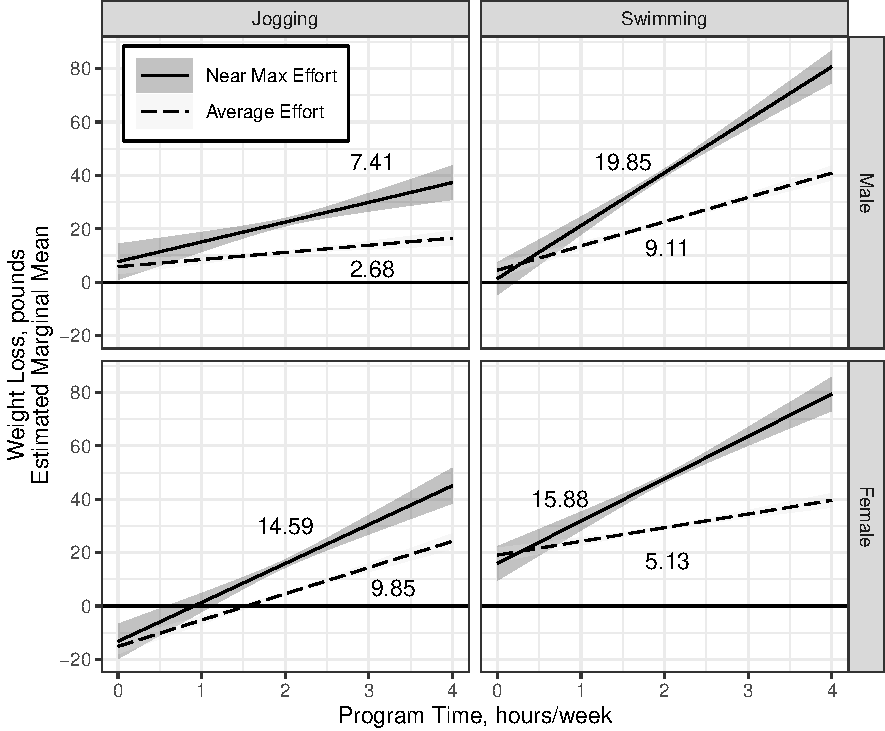
\includegraphics{Appendix_ex_weightloss_files/figure-latex/unnamed-chunk-101-1} \hfill{}

\caption{RQ (3) Compare Effort Discrepincies in Additional Weight Loss Associated with an Hour Increase per Week in Each Exercise Program, by Gender}\label{fig:unnamed-chunk-101}
\end{figure}

\clearpage

\hypertarget{conclusion-2}{%
\subsubsection{Conclusion}\label{conclusion-2}}

For the jogging program, both males and females with high effort can
expect to loose an additional 1.07 pound on average for every one hour
increase in exercise compared to people who put in average effort. This
discrepancy is 2.43 for the swimming program.

\clearpage

\hypertarget{session-information}{%
\section{SESSION INFORMATION}\label{session-information}}

\begin{Shaded}
\begin{Highlighting}[]
\FunctionTok{sessionInfo}\NormalTok{()}
\end{Highlighting}
\end{Shaded}

\begin{verbatim}
R version 4.3.1 (2023-06-16 ucrt)
Platform: x86_64-w64-mingw32/x64 (64-bit)
Running under: Windows 11 x64 (build 22631)

Matrix products: default


locale:
[1] LC_COLLATE=English_United States.utf8 
[2] LC_CTYPE=English_United States.utf8   
[3] LC_MONETARY=English_United States.utf8
[4] LC_NUMERIC=C                          
[5] LC_TIME=English_United States.utf8    

time zone: America/Denver
tzcode source: internal

attached base packages:
[1] stats     graphics  grDevices utils     datasets  methods   base     

other attached packages:
 [1] performance_0.11.0 interactions_1.1.5 emmeans_1.10.1     texreg_1.39.3     
 [5] DHARMa_0.4.6       olsrr_0.6.0        MOTE_1.0.2         ggpubr_0.6.0      
 [9] rstatix_0.7.2      naniar_1.1.0       flextable_0.9.5    psych_2.4.3       
[13] furniture_1.9.14   lubridate_1.9.3    forcats_1.0.0      stringr_1.5.1     
[17] dplyr_1.1.4        purrr_1.0.2        readr_2.1.5        tidyr_1.3.1       
[21] tibble_3.2.1       ggplot2_3.5.0      tidyverse_2.0.0    apaSupp_0.0.0.9000

loaded via a namespace (and not attached):
  [1] rstudioapi_0.16.0       jsonlite_1.8.8          magrittr_2.0.3         
  [4] TH.data_1.1-2           estimability_1.5        corrplot_0.92          
  [7] farver_2.1.1            nloptr_2.0.3            rmarkdown_2.26         
 [10] ragg_1.3.0              vctrs_0.6.5             minqa_1.2.6            
 [13] askpass_1.2.0           tinytex_0.50            htmltools_0.5.8.1      
 [16] curl_5.2.1              survey_4.4-2            broom_1.0.5            
 [19] sass_0.4.9              bslib_0.7.0             plyr_1.8.9             
 [22] sandwich_3.1-0          cachem_1.0.8            zoo_1.8-12             
 [25] gt_0.10.1               uuid_1.2-0              mime_0.12              
 [28] lifecycle_1.0.4         pkgconfig_2.0.3         Matrix_1.6-5           
 [31] R6_2.5.1                fastmap_1.1.1           shiny_1.8.1.1          
 [34] digest_0.6.35           colorspace_2.1-0        reshape_0.8.9          
 [37] textshaping_0.3.7       labeling_0.4.3          effects_4.2-2          
 [40] fansi_1.0.6             timechange_0.3.0        httr_1.4.7             
 [43] abind_1.4-5             mgcv_1.9-1              compiler_4.3.1         
 [46] fontquiver_0.2.1        withr_3.0.0             pander_0.6.5           
 [49] backports_1.4.1         DBI_1.2.2               carData_3.0-5          
 [52] ggsignif_0.6.4          MASS_7.3-60             openssl_2.1.1          
 [55] gfonts_0.2.0            tools_4.3.1             zip_2.3.1              
 [58] httpuv_1.6.15           visdat_0.6.0            nnet_7.3-19            
 [61] goftest_1.2-3           glue_1.7.0              nlme_3.1-164           
 [64] promises_1.3.0          grid_4.3.1              reshape2_1.4.4         
 [67] generics_0.1.3          rempsyc_0.1.7           gtable_0.3.4           
 [70] MBESS_4.9.3             nortest_1.0-4           tzdb_0.4.0             
 [73] data.table_1.15.4       hms_1.1.3               xml2_1.3.6             
 [76] car_3.1-2               utf8_1.2.4              pillar_1.9.0           
 [79] later_1.3.2             mitools_2.4             splines_4.3.1          
 [82] lattice_0.21-8          survival_3.5-8          tidyselect_1.2.1       
 [85] fontLiberation_0.1.0    knitr_1.46              fontBitstreamVera_0.1.1
 [88] gridExtra_2.3           crul_1.4.2              xfun_0.43              
 [91] stringi_1.8.3           yaml_2.3.8              boot_1.3-28.1          
 [94] evaluate_0.23           codetools_0.2-19        httpcode_0.3.0         
 [97] officer_0.6.5           gdtools_0.3.7           cli_3.6.2              
[100] xtable_1.8-4            systemfonts_1.0.6       jquerylib_0.1.4        
[103] munsell_0.5.1           Rcpp_1.0.12             coda_0.19-4.1          
[106] parallel_4.3.1          lme4_1.1-35.2           mvtnorm_1.2-4          
[109] scales_1.3.0            ez_4.4-0                insight_0.19.10        
[112] crayon_1.5.2            rlang_1.1.3             multcomp_1.4-25        
[115] mnormt_2.1.1            jtools_2.2.2           
\end{verbatim}

\clearpage

\hypertarget{bibliography}{%
\section{BIBLIOGRAPHY}\label{bibliography}}

\doublespacing

\hypertarget{refs}{}
\begin{CSLReferences}{1}{0}
\leavevmode\vadjust pre{\hypertarget{ref-RJ-2017-037}{}}%
Barrett, T. S., \& Brignone, E. (2017). Furniture for quantitative
scientists. \emph{The R Journal}, \emph{9}(2), 142--148.
\url{https://doi.org/10.32614/RJ-2017-037}

\leavevmode\vadjust pre{\hypertarget{ref-R-furniture}{}}%
Barrett, T. S., Brignone, E., \& Laxman, D. J. (2023). \emph{Furniture:
Furniture for quantitative scientists}.
\url{https://CRAN.R-project.org/package=furniture}

\leavevmode\vadjust pre{\hypertarget{ref-R-MOTE}{}}%
Buchanan, E. M., Gillenwaters, A. M., Scofield, J. E., \& Valentine, K.
D. (2019). \emph{MOTE: Effect size and confidence interval calculator}.
\url{https://CRAN.R-project.org/package=MOTE}

\leavevmode\vadjust pre{\hypertarget{ref-R-flextable}{}}%
Gohel, D., \& Skintzos, P. (2024). \emph{Flextable: Functions for
tabular reporting}. \url{https://ardata-fr.github.io/flextable-book/}

\leavevmode\vadjust pre{\hypertarget{ref-lubridate2011}{}}%
Grolemund, G., \& Wickham, H. (2011). Dates and times made easy with
{lubridate}. \emph{Journal of Statistical Software}, \emph{40}(3),
1--25. \url{https://www.jstatsoft.org/v40/i03/}

\leavevmode\vadjust pre{\hypertarget{ref-R-DHARMa}{}}%
Hartig, F. (2022). \emph{DHARMa: Residual diagnostics for hierarchical
(multi-level / mixed) regression models}.
\url{http://florianhartig.github.io/DHARMa/}

\leavevmode\vadjust pre{\hypertarget{ref-R-olsrr}{}}%
Hebbali, A. (2024). \emph{Olsrr: Tools for building OLS regression
models}. \url{https://olsrr.rsquaredacademy.com/}

\leavevmode\vadjust pre{\hypertarget{ref-R-ggpubr}{}}%
Kassambara, A. (2023a). \emph{Ggpubr: ggplot2 based publication ready
plots}. \url{https://rpkgs.datanovia.com/ggpubr/}

\leavevmode\vadjust pre{\hypertarget{ref-R-rstatix}{}}%
Kassambara, A. (2023b). \emph{Rstatix: Pipe-friendly framework for basic
statistical tests}. \url{https://rpkgs.datanovia.com/rstatix/}

\leavevmode\vadjust pre{\hypertarget{ref-texreg2013}{}}%
Leifeld, P. (2013). {texreg}: Conversion of statistical model output in
{R} to {LaTeX} and {HTML} tables. \emph{Journal of Statistical
Software}, \emph{55}(8), 1--24.
\url{https://doi.org/10.18637/jss.v055.i08}

\leavevmode\vadjust pre{\hypertarget{ref-R-texreg}{}}%
Leifeld, P. (2023). \emph{Texreg: Conversion of r regression output to
LaTeX or HTML tables}. \url{https://github.com/leifeld/texreg/}

\leavevmode\vadjust pre{\hypertarget{ref-R-emmeans}{}}%
Lenth, R. V. (2024). \emph{Emmeans: Estimated marginal means, aka
least-squares means}. \url{https://github.com/rvlenth/emmeans}

\leavevmode\vadjust pre{\hypertarget{ref-R-interactions}{}}%
Long, J. A. (2021). \emph{Interactions: Comprehensive, user-friendly
toolkit for probing interactions}.
\url{https://interactions.jacob-long.com}

\leavevmode\vadjust pre{\hypertarget{ref-performance2021}{}}%
Lüdecke, D., Ben-Shachar, M. S., Patil, I., Waggoner, P., \& Makowski,
D. (2021). {performance}: An {R} package for assessment, comparison and
testing of statistical models. \emph{Journal of Open Source Software},
\emph{6}(60), 3139. \url{https://doi.org/10.21105/joss.03139}

\leavevmode\vadjust pre{\hypertarget{ref-R-performance}{}}%
Lüdecke, D., Makowski, D., Ben-Shachar, M. S., Patil, I., Waggoner, P.,
Wiernik, B. M., \& Thériault, R. (2024). \emph{Performance: Assessment
of regression models performance}.
\url{https://easystats.github.io/performance/}

\leavevmode\vadjust pre{\hypertarget{ref-R-tibble}{}}%
Müller, K., \& Wickham, H. (2023). \emph{Tibble: Simple data frames}.
\url{https://tibble.tidyverse.org/}

\leavevmode\vadjust pre{\hypertarget{ref-R-base}{}}%
R Core Team. (2023). \emph{R: A language and environment for statistical
computing}. R Foundation for Statistical Computing.
\url{https://www.R-project.org/}

\leavevmode\vadjust pre{\hypertarget{ref-R-psych}{}}%
Revelle, W. (2024). \emph{Psych: Procedures for psychological,
psychometric, and personality research}.
\href{https://personality-project.org/r/psych/\%0Ahttps://personality-project.org/r/psych-manual.pdf}{https://personality-project.org/r/psych/
https://personality-project.org/r/psych-manual.pdf}

\leavevmode\vadjust pre{\hypertarget{ref-R-apaSupp}{}}%
Schwartz, S. (2024). \emph{apaSupp: APA formatted supplemental
materials}. \url{https://github.com/SarBearSchwartz/apaSupp}

\leavevmode\vadjust pre{\hypertarget{ref-apaSupp2024}{}}%
Schwartz, S. E. (2024). apaSup: An r package for preparing supplemental
material, APA 7th ed. \emph{Open Science Framework}.
\url{https://doi.org/10.17605/OSF.IO/G38JN}

\leavevmode\vadjust pre{\hypertarget{ref-R-lubridate}{}}%
Spinu, V., Grolemund, G., \& Wickham, H. (2023). \emph{Lubridate: Make
dealing with dates a little easier}.
\url{https://lubridate.tidyverse.org}

\leavevmode\vadjust pre{\hypertarget{ref-naniar2023}{}}%
Tierney, N., \& Cook, D. (2023). Expanding tidy data principles to
facilitate missing data exploration, visualization and assessment of
imputations. \emph{Journal of Statistical Software}, \emph{105}(7),
1--31. \url{https://doi.org/10.18637/jss.v105.i07}

\leavevmode\vadjust pre{\hypertarget{ref-R-naniar}{}}%
Tierney, N., Cook, D., McBain, M., \& Fay, C. (2024). \emph{Naniar: Data
structures, summaries, and visualisations for missing data}.
\url{https://github.com/njtierney/naniar}

\leavevmode\vadjust pre{\hypertarget{ref-ggplot22016}{}}%
Wickham, H. (2016). \emph{ggplot2: Elegant graphics for data analysis}.
Springer-Verlag New York. \url{https://ggplot2.tidyverse.org}

\leavevmode\vadjust pre{\hypertarget{ref-R-forcats}{}}%
Wickham, H. (2023a). \emph{Forcats: Tools for working with categorical
variables (factors)}. \url{https://forcats.tidyverse.org/}

\leavevmode\vadjust pre{\hypertarget{ref-R-stringr}{}}%
Wickham, H. (2023b). \emph{Stringr: Simple, consistent wrappers for
common string operations}. \url{https://stringr.tidyverse.org}

\leavevmode\vadjust pre{\hypertarget{ref-R-tidyverse}{}}%
Wickham, H. (2023c). \emph{Tidyverse: Easily install and load the
tidyverse}. \url{https://tidyverse.tidyverse.org}

\leavevmode\vadjust pre{\hypertarget{ref-tidyverse2019}{}}%
Wickham, H., Averick, M., Bryan, J., Chang, W., McGowan, L. D.,
François, R., Grolemund, G., Hayes, A., Henry, L., Hester, J., Kuhn, M.,
Pedersen, T. L., Miller, E., Bache, S. M., Müller, K., Ooms, J.,
Robinson, D., Seidel, D. P., Spinu, V., \ldots{} Yutani, H. (2019).
Welcome to the {tidyverse}. \emph{Journal of Open Source Software},
\emph{4}(43), 1686. \url{https://doi.org/10.21105/joss.01686}

\leavevmode\vadjust pre{\hypertarget{ref-R-ggplot2}{}}%
Wickham, H., Chang, W., Henry, L., Pedersen, T. L., Takahashi, K.,
Wilke, C., Woo, K., Yutani, H., Dunnington, D., \& van den Brand, T.
(2024). \emph{ggplot2: Create elegant data visualisations using the
grammar of graphics}. \url{https://ggplot2.tidyverse.org}

\leavevmode\vadjust pre{\hypertarget{ref-R-dplyr}{}}%
Wickham, H., François, R., Henry, L., Müller, K., \& Vaughan, D. (2023).
\emph{Dplyr: A grammar of data manipulation}.
\url{https://dplyr.tidyverse.org}

\leavevmode\vadjust pre{\hypertarget{ref-R-purrr}{}}%
Wickham, H., \& Henry, L. (2023). \emph{Purrr: Functional programming
tools}. \url{https://purrr.tidyverse.org/}

\leavevmode\vadjust pre{\hypertarget{ref-R-readr}{}}%
Wickham, H., Hester, J., \& Bryan, J. (2024). \emph{Readr: Read
rectangular text data}. \url{https://readr.tidyverse.org}

\leavevmode\vadjust pre{\hypertarget{ref-R-tidyr}{}}%
Wickham, H., Vaughan, D., \& Girlich, M. (2024). \emph{Tidyr: Tidy messy
data}. \url{https://tidyr.tidyverse.org}

\end{CSLReferences}

\end{document}
